The traction jump $\ff$ minimizes the energy functional
$\int_{\gamma}\frac{\kappa_{b}}{2}\kappa^{2}ds$ subject to the
inextensibility constraint.  An alternative traction jump is derived by
minimizing
\begin{align}
  \int_{\gamma}\frac{\kappa_{b}}{2}(\kappa - \tilde{\kappa})^{2}ds, \quad \text{subject to} \quad \|\xx_{s}\|=1,
    \label{e:new:bending}
\end{align}
where $\tilde{\kappa}$ is the curvature of a prescribed intrinsic
vesicle shape whose perimeter we are assuming is one.  By taking the
first variation of~\eqref{e:new:bending}, the force due to bending is
\begin{align*}
  \mathbf{f}_{b} = \left(\kappa_{ss} + \frac{\kappa^{3}}{2} -
    \tilde{\kappa}_{ss} - \frac{\kappa\tilde{\kappa}^{2}}{2}\right)\mathbf{n} + 
    (\kappa-\tilde{\kappa})\tilde{\kappa}_{s}\mathbf{t}.
\end{align*}
It is shown in~\cite{shravan} that terms of the form
$(h(s)\xx_{s})_{s}$ do no work for inextensible vesicles and hence
such forces can be added to modify $\mathbf{f}_{b}$.  A convenient
choice is $h(s) = 3/2\, \kappa^{2} - 1/2\, \tilde{\kappa}^{2}$ which
results in the simpler traction jump
\begin{align*}
  \ff = \ff_{b} + \ff_{\sigma} = \kappa_{b}(-\xx_{ssss} - \tilde{\kappa}_{ss} \mathbf{n} - 
    \kappa \tilde{\kappa}_{s}\mathbf{t}) + (\sigma \xx_{s})_{s}.
\end{align*}

We present simulations for several choices of $\tilde{\kappa}$ in
Figure~\ref{f:newbending}.  The flow is only driven by the vesicle
configuration since there is no background flow.  For $\tilde{\kappa}$,
we take the curvature of an ellipse with an aspect ratio of 1 (top
plots), 2 (middle plots), and 4 (bottom plots).  We see that the
curvature of the vesicle tries to fit to the curvature of the intrinsic
shape while maintaining its area and arclength.

\begin{figure}[htp]
\begin{center}
  \begin{tabular}{c@{\,}c@{\,}c@{\,}c@{\,}c@{\,}c@{\,}}
    \ifInputs
    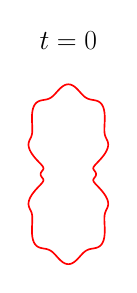
\begin{tikzpicture}[scale=0.4]

\begin{axis}[
  xmin = -1,
  xmax = 1,
  ymin = -2,
  ymax = 2,
  scale only axis,
  axis equal image,
  hide axis,
  title = {\Huge$t=0$}
  ]

\addplot [mark=none,red,line width=1.5] table{
4.8450e-01 0.0000e+00
4.8282e-01 1.3944e-02
4.7797e-01 2.7625e-02
4.7057e-01 4.0837e-02
4.6157e-01 5.3483e-02
4.5216e-01 6.5610e-02
4.4368e-01 7.7429e-02
4.3749e-01 8.9309e-02
4.3482e-01 1.0175e-01
4.3664e-01 1.1536e-01
4.4363e-01 1.3073e-01
4.5602e-01 1.4847e-01
4.7362e-01 1.6902e-01
4.9581e-01 1.9270e-01
5.2161e-01 2.1957e-01
5.4970e-01 2.4946e-01
5.7862e-01 2.8197e-01
6.0680e-01 3.1644e-01
6.3277e-01 3.5209e-01
6.5522e-01 3.8801e-01
6.7317e-01 4.2331e-01
6.8596e-01 4.5717e-01
6.9337e-01 4.8893e-01
6.9559e-01 5.1821e-01
6.9318e-01 5.4490e-01
6.8700e-01 5.6922e-01
6.7816e-01 5.9171e-01
6.6784e-01 6.1317e-01
6.5726e-01 6.3458e-01
6.4746e-01 6.5706e-01
6.3932e-01 6.8170e-01
6.3339e-01 7.0946e-01
6.2991e-01 7.4107e-01
6.2877e-01 7.7696e-01
6.2953e-01 8.1715e-01
6.3150e-01 8.6127e-01
6.3378e-01 9.0854e-01
6.3539e-01 9.5785e-01
6.3533e-01 1.0078e+00
6.3270e-01 1.0569e+00
6.2678e-01 1.1036e+00
6.1707e-01 1.1464e+00
6.0334e-01 1.1842e+00
5.8565e-01 1.2163e+00
5.6432e-01 1.2421e+00
5.3988e-01 1.2618e+00
5.1301e-01 1.2761e+00
4.8448e-01 1.2859e+00
4.5506e-01 1.2925e+00
4.2543e-01 1.2975e+00
3.9616e-01 1.3026e+00
3.6763e-01 1.3092e+00
3.4002e-01 1.3187e+00
3.1334e-01 1.3321e+00
2.8738e-01 1.3498e+00
2.6183e-01 1.3718e+00
2.3629e-01 1.3975e+00
2.1033e-01 1.4261e+00
1.8358e-01 1.4560e+00
1.5574e-01 1.4856e+00
1.2667e-01 1.5130e+00
9.6346e-02 1.5366e+00
6.4922e-02 1.5547e+00
3.2679e-02 1.5661e+00
8.1715e-17 1.5700e+00
-3.2679e-02 1.5661e+00
-6.4922e-02 1.5547e+00
-9.6346e-02 1.5366e+00
-1.2667e-01 1.5130e+00
-1.5574e-01 1.4856e+00
-1.8358e-01 1.4560e+00
-2.1033e-01 1.4261e+00
-2.3629e-01 1.3975e+00
-2.6183e-01 1.3718e+00
-2.8738e-01 1.3498e+00
-3.1334e-01 1.3321e+00
-3.4002e-01 1.3187e+00
-3.6763e-01 1.3092e+00
-3.9616e-01 1.3026e+00
-4.2543e-01 1.2975e+00
-4.5506e-01 1.2925e+00
-4.8448e-01 1.2859e+00
-5.1301e-01 1.2761e+00
-5.3988e-01 1.2618e+00
-5.6432e-01 1.2421e+00
-5.8565e-01 1.2163e+00
-6.0334e-01 1.1842e+00
-6.1707e-01 1.1464e+00
-6.2678e-01 1.1036e+00
-6.3270e-01 1.0569e+00
-6.3533e-01 1.0078e+00
-6.3539e-01 9.5785e-01
-6.3378e-01 9.0854e-01
-6.3150e-01 8.6127e-01
-6.2953e-01 8.1715e-01
-6.2877e-01 7.7696e-01
-6.2991e-01 7.4107e-01
-6.3339e-01 7.0946e-01
-6.3932e-01 6.8170e-01
-6.4746e-01 6.5706e-01
-6.5726e-01 6.3458e-01
-6.6784e-01 6.1317e-01
-6.7816e-01 5.9171e-01
-6.8700e-01 5.6922e-01
-6.9318e-01 5.4490e-01
-6.9559e-01 5.1821e-01
-6.9337e-01 4.8893e-01
-6.8596e-01 4.5717e-01
-6.7317e-01 4.2331e-01
-6.5522e-01 3.8801e-01
-6.3277e-01 3.5209e-01
-6.0680e-01 3.1644e-01
-5.7862e-01 2.8197e-01
-5.4970e-01 2.4946e-01
-5.2161e-01 2.1957e-01
-4.9581e-01 1.9270e-01
-4.7362e-01 1.6902e-01
-4.5602e-01 1.4847e-01
-4.4363e-01 1.3073e-01
-4.3664e-01 1.1536e-01
-4.3482e-01 1.0175e-01
-4.3749e-01 8.9309e-02
-4.4368e-01 7.7429e-02
-4.5216e-01 6.5610e-02
-4.6157e-01 5.3483e-02
-4.7057e-01 4.0837e-02
-4.7797e-01 2.7625e-02
-4.8282e-01 1.3944e-02
-4.8450e-01 6.9805e-17
-4.8282e-01 -1.3944e-02
-4.7797e-01 -2.7625e-02
-4.7057e-01 -4.0837e-02
-4.6157e-01 -5.3483e-02
-4.5216e-01 -6.5610e-02
-4.4368e-01 -7.7429e-02
-4.3749e-01 -8.9309e-02
-4.3482e-01 -1.0175e-01
-4.3664e-01 -1.1536e-01
-4.4363e-01 -1.3073e-01
-4.5602e-01 -1.4847e-01
-4.7362e-01 -1.6902e-01
-4.9581e-01 -1.9270e-01
-5.2161e-01 -2.1957e-01
-5.4970e-01 -2.4946e-01
-5.7862e-01 -2.8197e-01
-6.0680e-01 -3.1644e-01
-6.3277e-01 -3.5209e-01
-6.5522e-01 -3.8801e-01
-6.7317e-01 -4.2331e-01
-6.8596e-01 -4.5717e-01
-6.9337e-01 -4.8893e-01
-6.9559e-01 -5.1821e-01
-6.9318e-01 -5.4490e-01
-6.8700e-01 -5.6922e-01
-6.7816e-01 -5.9171e-01
-6.6784e-01 -6.1317e-01
-6.5726e-01 -6.3458e-01
-6.4746e-01 -6.5706e-01
-6.3932e-01 -6.8170e-01
-6.3339e-01 -7.0946e-01
-6.2991e-01 -7.4107e-01
-6.2877e-01 -7.7696e-01
-6.2953e-01 -8.1715e-01
-6.3150e-01 -8.6127e-01
-6.3378e-01 -9.0854e-01
-6.3539e-01 -9.5785e-01
-6.3533e-01 -1.0078e+00
-6.3270e-01 -1.0569e+00
-6.2678e-01 -1.1036e+00
-6.1707e-01 -1.1464e+00
-6.0334e-01 -1.1842e+00
-5.8565e-01 -1.2163e+00
-5.6432e-01 -1.2421e+00
-5.3988e-01 -1.2618e+00
-5.1301e-01 -1.2761e+00
-4.8448e-01 -1.2859e+00
-4.5506e-01 -1.2925e+00
-4.2543e-01 -1.2975e+00
-3.9616e-01 -1.3026e+00
-3.6763e-01 -1.3092e+00
-3.4002e-01 -1.3187e+00
-3.1334e-01 -1.3321e+00
-2.8738e-01 -1.3498e+00
-2.6183e-01 -1.3718e+00
-2.3629e-01 -1.3975e+00
-2.1033e-01 -1.4261e+00
-1.8358e-01 -1.4560e+00
-1.5574e-01 -1.4856e+00
-1.2667e-01 -1.5130e+00
-9.6346e-02 -1.5366e+00
-6.4922e-02 -1.5547e+00
-3.2679e-02 -1.5661e+00
-2.4514e-16 -1.5700e+00
3.2679e-02 -1.5661e+00
6.4922e-02 -1.5547e+00
9.6346e-02 -1.5366e+00
1.2667e-01 -1.5130e+00
1.5574e-01 -1.4856e+00
1.8358e-01 -1.4560e+00
2.1033e-01 -1.4261e+00
2.3629e-01 -1.3975e+00
2.6183e-01 -1.3718e+00
2.8738e-01 -1.3498e+00
3.1334e-01 -1.3321e+00
3.4002e-01 -1.3187e+00
3.6763e-01 -1.3092e+00
3.9616e-01 -1.3026e+00
4.2543e-01 -1.2975e+00
4.5506e-01 -1.2925e+00
4.8448e-01 -1.2859e+00
5.1301e-01 -1.2761e+00
5.3988e-01 -1.2618e+00
5.6432e-01 -1.2421e+00
5.8565e-01 -1.2163e+00
6.0334e-01 -1.1842e+00
6.1707e-01 -1.1464e+00
6.2678e-01 -1.1036e+00
6.3270e-01 -1.0569e+00
6.3533e-01 -1.0078e+00
6.3539e-01 -9.5785e-01
6.3378e-01 -9.0854e-01
6.3150e-01 -8.6127e-01
6.2953e-01 -8.1715e-01
6.2877e-01 -7.7696e-01
6.2991e-01 -7.4107e-01
6.3339e-01 -7.0946e-01
6.3932e-01 -6.8170e-01
6.4746e-01 -6.5706e-01
6.5726e-01 -6.3458e-01
6.6784e-01 -6.1317e-01
6.7816e-01 -5.9171e-01
6.8700e-01 -5.6922e-01
6.9318e-01 -5.4490e-01
6.9559e-01 -5.1821e-01
6.9337e-01 -4.8893e-01
6.8596e-01 -4.5717e-01
6.7317e-01 -4.2331e-01
6.5522e-01 -3.8801e-01
6.3277e-01 -3.5209e-01
6.0680e-01 -3.1644e-01
5.7862e-01 -2.8197e-01
5.4970e-01 -2.4946e-01
5.2161e-01 -2.1957e-01
4.9581e-01 -1.9270e-01
4.7362e-01 -1.6902e-01
4.5602e-01 -1.4847e-01
4.4363e-01 -1.3073e-01
4.3664e-01 -1.1536e-01
4.3482e-01 -1.0175e-01
4.3749e-01 -8.9309e-02
4.4368e-01 -7.7429e-02
4.5216e-01 -6.5610e-02
4.6157e-01 -5.3483e-02
4.7057e-01 -4.0837e-02
4.7797e-01 -2.7625e-02
4.8282e-01 -1.3944e-02
4.8450e-01 0.0000e+00
};


\end{axis}

\end{tikzpicture}



 &
    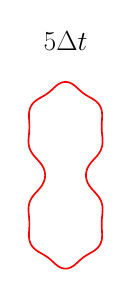
\begin{tikzpicture}[scale=0.4]

\begin{axis}[
  xmin = -1,
  xmax = 1,
  ymin = -2,
  ymax = 2,
  scale only axis,
  axis equal image,
  hide axis,
  title = {\Huge$5\Delta t$}
  ]

\addplot [mark=none,red,line width=1.5] table{
3.5689e-01 4.3470e-13
3.5723e-01 1.4105e-02
3.5830e-01 2.8811e-02
3.6024e-01 4.4340e-02
3.6311e-01 6.0387e-02
3.6684e-01 7.6223e-02
3.7112e-01 9.1011e-02
3.7564e-01 1.0426e-01
3.8035e-01 1.1640e-01
3.8591e-01 1.2916e-01
3.9344e-01 1.4456e-01
4.0408e-01 1.6366e-01
4.1874e-01 1.8657e-01
4.3804e-01 2.1283e-01
4.6191e-01 2.4160e-01
4.8951e-01 2.7216e-01
5.1918e-01 3.0418e-01
5.4875e-01 3.3764e-01
5.7594e-01 3.7242e-01
5.9894e-01 4.0801e-01
6.1679e-01 4.4336e-01
6.2953e-01 4.7727e-01
6.3789e-01 5.0887e-01
6.4291e-01 5.3787e-01
6.4558e-01 5.6460e-01
6.4660e-01 5.8974e-01
6.4644e-01 6.1399e-01
6.4539e-01 6.3786e-01
6.4368e-01 6.6178e-01
6.4148e-01 6.8627e-01
6.3894e-01 7.1213e-01
6.3619e-01 7.4042e-01
6.3351e-01 7.7216e-01
6.3141e-01 8.0804e-01
6.3052e-01 8.4825e-01
6.3139e-01 8.9241e-01
6.3396e-01 9.3968e-01
6.3718e-01 9.8893e-01
6.3903e-01 1.0389e+00
6.3721e-01 1.0880e+00
6.3003e-01 1.1345e+00
6.1722e-01 1.1765e+00
5.9982e-01 1.2128e+00
5.7946e-01 1.2433e+00
5.5746e-01 1.2686e+00
5.3443e-01 1.2901e+00
5.1045e-01 1.3089e+00
4.8548e-01 1.3259e+00
4.5971e-01 1.3417e+00
4.3360e-01 1.3567e+00
4.0767e-01 1.3714e+00
3.8224e-01 1.3860e+00
3.5724e-01 1.4012e+00
3.3223e-01 1.4176e+00
3.0666e-01 1.4359e+00
2.8016e-01 1.4567e+00
2.5267e-01 1.4804e+00
2.2425e-01 1.5066e+00
1.9488e-01 1.5339e+00
1.6433e-01 1.5607e+00
1.3245e-01 1.5849e+00
9.9476e-02 1.6046e+00
6.6053e-02 1.6188e+00
3.2840e-02 1.6270e+00
4.1798e-13 1.6297e+00
-3.2840e-02 1.6270e+00
-6.6053e-02 1.6188e+00
-9.9476e-02 1.6046e+00
-1.3245e-01 1.5849e+00
-1.6433e-01 1.5607e+00
-1.9488e-01 1.5339e+00
-2.2425e-01 1.5066e+00
-2.5267e-01 1.4804e+00
-2.8016e-01 1.4567e+00
-3.0666e-01 1.4359e+00
-3.3223e-01 1.4176e+00
-3.5724e-01 1.4012e+00
-3.8224e-01 1.3860e+00
-4.0767e-01 1.3714e+00
-4.3360e-01 1.3567e+00
-4.5971e-01 1.3417e+00
-4.8548e-01 1.3259e+00
-5.1045e-01 1.3089e+00
-5.3443e-01 1.2901e+00
-5.5746e-01 1.2686e+00
-5.7946e-01 1.2433e+00
-5.9982e-01 1.2128e+00
-6.1722e-01 1.1765e+00
-6.3003e-01 1.1345e+00
-6.3721e-01 1.0880e+00
-6.3903e-01 1.0389e+00
-6.3718e-01 9.8893e-01
-6.3396e-01 9.3968e-01
-6.3139e-01 8.9241e-01
-6.3052e-01 8.4825e-01
-6.3141e-01 8.0804e-01
-6.3351e-01 7.7216e-01
-6.3619e-01 7.4042e-01
-6.3894e-01 7.1213e-01
-6.4148e-01 6.8627e-01
-6.4368e-01 6.6178e-01
-6.4539e-01 6.3786e-01
-6.4644e-01 6.1399e-01
-6.4660e-01 5.8974e-01
-6.4558e-01 5.6460e-01
-6.4291e-01 5.3787e-01
-6.3789e-01 5.0887e-01
-6.2953e-01 4.7727e-01
-6.1679e-01 4.4336e-01
-5.9894e-01 4.0801e-01
-5.7594e-01 3.7242e-01
-5.4875e-01 3.3764e-01
-5.1918e-01 3.0418e-01
-4.8951e-01 2.7216e-01
-4.6191e-01 2.4160e-01
-4.3804e-01 2.1283e-01
-4.1874e-01 1.8657e-01
-4.0408e-01 1.6366e-01
-3.9344e-01 1.4456e-01
-3.8591e-01 1.2916e-01
-3.8035e-01 1.1640e-01
-3.7564e-01 1.0426e-01
-3.7112e-01 9.1011e-02
-3.6684e-01 7.6223e-02
-3.6311e-01 6.0387e-02
-3.6024e-01 4.4340e-02
-3.5830e-01 2.8811e-02
-3.5723e-01 1.4105e-02
-3.5689e-01 -9.0549e-13
-3.5723e-01 -1.4105e-02
-3.5830e-01 -2.8811e-02
-3.6024e-01 -4.4340e-02
-3.6311e-01 -6.0387e-02
-3.6684e-01 -7.6223e-02
-3.7112e-01 -9.1011e-02
-3.7564e-01 -1.0426e-01
-3.8035e-01 -1.1640e-01
-3.8591e-01 -1.2916e-01
-3.9344e-01 -1.4456e-01
-4.0408e-01 -1.6366e-01
-4.1874e-01 -1.8657e-01
-4.3804e-01 -2.1283e-01
-4.6191e-01 -2.4160e-01
-4.8951e-01 -2.7216e-01
-5.1918e-01 -3.0418e-01
-5.4875e-01 -3.3764e-01
-5.7594e-01 -3.7242e-01
-5.9894e-01 -4.0801e-01
-6.1679e-01 -4.4336e-01
-6.2953e-01 -4.7727e-01
-6.3789e-01 -5.0887e-01
-6.4291e-01 -5.3787e-01
-6.4558e-01 -5.6460e-01
-6.4660e-01 -5.8974e-01
-6.4644e-01 -6.1399e-01
-6.4539e-01 -6.3786e-01
-6.4368e-01 -6.6178e-01
-6.4148e-01 -6.8627e-01
-6.3894e-01 -7.1213e-01
-6.3619e-01 -7.4042e-01
-6.3351e-01 -7.7216e-01
-6.3141e-01 -8.0804e-01
-6.3052e-01 -8.4825e-01
-6.3139e-01 -8.9241e-01
-6.3396e-01 -9.3968e-01
-6.3718e-01 -9.8893e-01
-6.3903e-01 -1.0389e+00
-6.3721e-01 -1.0880e+00
-6.3003e-01 -1.1345e+00
-6.1722e-01 -1.1765e+00
-5.9982e-01 -1.2128e+00
-5.7946e-01 -1.2433e+00
-5.5746e-01 -1.2686e+00
-5.3443e-01 -1.2901e+00
-5.1045e-01 -1.3089e+00
-4.8548e-01 -1.3259e+00
-4.5971e-01 -1.3417e+00
-4.3360e-01 -1.3567e+00
-4.0767e-01 -1.3714e+00
-3.8224e-01 -1.3860e+00
-3.5724e-01 -1.4012e+00
-3.3223e-01 -1.4176e+00
-3.0666e-01 -1.4359e+00
-2.8016e-01 -1.4567e+00
-2.5267e-01 -1.4804e+00
-2.2425e-01 -1.5066e+00
-1.9488e-01 -1.5339e+00
-1.6433e-01 -1.5607e+00
-1.3245e-01 -1.5849e+00
-9.9476e-02 -1.6046e+00
-6.6053e-02 -1.6188e+00
-3.2840e-02 -1.6270e+00
-2.6155e-13 -1.6297e+00
3.2840e-02 -1.6270e+00
6.6053e-02 -1.6188e+00
9.9476e-02 -1.6046e+00
1.3245e-01 -1.5849e+00
1.6433e-01 -1.5607e+00
1.9488e-01 -1.5339e+00
2.2425e-01 -1.5066e+00
2.5267e-01 -1.4804e+00
2.8016e-01 -1.4567e+00
3.0666e-01 -1.4359e+00
3.3223e-01 -1.4176e+00
3.5724e-01 -1.4012e+00
3.8224e-01 -1.3860e+00
4.0767e-01 -1.3714e+00
4.3360e-01 -1.3567e+00
4.5971e-01 -1.3417e+00
4.8548e-01 -1.3259e+00
5.1045e-01 -1.3089e+00
5.3443e-01 -1.2901e+00
5.5746e-01 -1.2686e+00
5.7946e-01 -1.2433e+00
5.9982e-01 -1.2128e+00
6.1722e-01 -1.1765e+00
6.3003e-01 -1.1345e+00
6.3721e-01 -1.0880e+00
6.3903e-01 -1.0389e+00
6.3718e-01 -9.8893e-01
6.3396e-01 -9.3968e-01
6.3139e-01 -8.9241e-01
6.3052e-01 -8.4825e-01
6.3141e-01 -8.0804e-01
6.3351e-01 -7.7216e-01
6.3619e-01 -7.4042e-01
6.3894e-01 -7.1213e-01
6.4148e-01 -6.8627e-01
6.4368e-01 -6.6178e-01
6.4539e-01 -6.3786e-01
6.4644e-01 -6.1399e-01
6.4660e-01 -5.8974e-01
6.4558e-01 -5.6460e-01
6.4291e-01 -5.3787e-01
6.3789e-01 -5.0887e-01
6.2953e-01 -4.7727e-01
6.1679e-01 -4.4336e-01
5.9894e-01 -4.0801e-01
5.7594e-01 -3.7242e-01
5.4875e-01 -3.3764e-01
5.1918e-01 -3.0418e-01
4.8951e-01 -2.7216e-01
4.6191e-01 -2.4160e-01
4.3804e-01 -2.1283e-01
4.1874e-01 -1.8657e-01
4.0408e-01 -1.6366e-01
3.9344e-01 -1.4456e-01
3.8591e-01 -1.2916e-01
3.8035e-01 -1.1640e-01
3.7564e-01 -1.0426e-01
3.7112e-01 -9.1011e-02
3.6684e-01 -7.6223e-02
3.6311e-01 -6.0387e-02
3.6024e-01 -4.4340e-02
3.5830e-01 -2.8811e-02
3.5723e-01 -1.4105e-02
3.5689e-01 4.3470e-13
};


\end{axis}

\end{tikzpicture}



 &
    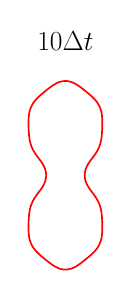
\begin{tikzpicture}[scale=0.4]

\begin{axis}[
  xmin = -1,
  xmax = 1,
  ymin = -2,
  ymax = 2,
  scale only axis,
  axis equal image,
  hide axis,
  title = {\Huge$10 \Delta t$}
  ]

\addplot [mark=none,red,line width=1.5] table{
3.3655e-01 -1.7698e-12
3.3686e-01 1.4106e-02
3.3784e-01 2.8818e-02
3.3961e-01 4.4368e-02
3.4224e-01 6.0459e-02
3.4563e-01 7.6370e-02
3.4952e-01 9.1266e-02
3.5361e-01 1.0465e-01
3.5787e-01 1.1696e-01
3.6288e-01 1.2994e-01
3.6966e-01 1.4570e-01
3.7919e-01 1.6537e-01
3.9227e-01 1.8923e-01
4.0941e-01 2.1695e-01
4.3053e-01 2.4780e-01
4.5492e-01 2.8099e-01
4.8121e-01 3.1586e-01
5.0768e-01 3.5183e-01
5.3261e-01 3.8828e-01
5.5468e-01 4.2446e-01
5.7318e-01 4.5949e-01
5.8804e-01 4.9255e-01
5.9962e-01 5.2313e-01
6.0856e-01 5.5119e-01
6.1553e-01 5.7715e-01
6.2107e-01 6.0171e-01
6.2559e-01 6.2555e-01
6.2933e-01 6.4917e-01
6.3245e-01 6.7297e-01
6.3508e-01 6.9743e-01
6.3734e-01 7.2333e-01
6.3932e-01 7.5170e-01
6.4105e-01 7.8352e-01
6.4252e-01 8.1944e-01
6.4368e-01 8.5965e-01
6.4432e-01 9.0381e-01
6.4398e-01 9.5115e-01
6.4192e-01 1.0005e+00
6.3719e-01 1.0503e+00
6.2902e-01 1.0988e+00
6.1720e-01 1.1443e+00
6.0221e-01 1.1856e+00
5.8500e-01 1.2221e+00
5.6659e-01 1.2537e+00
5.4759e-01 1.2814e+00
5.2815e-01 1.3062e+00
5.0806e-01 1.3292e+00
4.8712e-01 1.3510e+00
4.6535e-01 1.3720e+00
4.4304e-01 1.3923e+00
4.2056e-01 1.4119e+00
3.9811e-01 1.4308e+00
3.7555e-01 1.4494e+00
3.5237e-01 1.4683e+00
3.2786e-01 1.4880e+00
3.0138e-01 1.5089e+00
2.7262e-01 1.5311e+00
2.4150e-01 1.5539e+00
2.0826e-01 1.5764e+00
1.7337e-01 1.5973e+00
1.3755e-01 1.6152e+00
1.0173e-01 1.6292e+00
6.6728e-02 1.6389e+00
3.2923e-02 1.6444e+00
2.7884e-12 1.6462e+00
-3.2923e-02 1.6444e+00
-6.6728e-02 1.6389e+00
-1.0173e-01 1.6292e+00
-1.3755e-01 1.6152e+00
-1.7337e-01 1.5973e+00
-2.0826e-01 1.5764e+00
-2.4150e-01 1.5539e+00
-2.7262e-01 1.5311e+00
-3.0138e-01 1.5089e+00
-3.2786e-01 1.4880e+00
-3.5237e-01 1.4683e+00
-3.7555e-01 1.4494e+00
-3.9811e-01 1.4308e+00
-4.2056e-01 1.4119e+00
-4.4304e-01 1.3923e+00
-4.6535e-01 1.3720e+00
-4.8712e-01 1.3510e+00
-5.0806e-01 1.3292e+00
-5.2815e-01 1.3062e+00
-5.4759e-01 1.2814e+00
-5.6659e-01 1.2537e+00
-5.8500e-01 1.2221e+00
-6.0221e-01 1.1856e+00
-6.1720e-01 1.1443e+00
-6.2902e-01 1.0988e+00
-6.3719e-01 1.0503e+00
-6.4192e-01 1.0005e+00
-6.4398e-01 9.5115e-01
-6.4432e-01 9.0381e-01
-6.4368e-01 8.5965e-01
-6.4252e-01 8.1944e-01
-6.4105e-01 7.8352e-01
-6.3932e-01 7.5170e-01
-6.3734e-01 7.2333e-01
-6.3508e-01 6.9743e-01
-6.3245e-01 6.7297e-01
-6.2933e-01 6.4917e-01
-6.2559e-01 6.2555e-01
-6.2107e-01 6.0171e-01
-6.1553e-01 5.7715e-01
-6.0856e-01 5.5119e-01
-5.9962e-01 5.2313e-01
-5.8804e-01 4.9255e-01
-5.7318e-01 4.5949e-01
-5.5468e-01 4.2446e-01
-5.3261e-01 3.8828e-01
-5.0768e-01 3.5183e-01
-4.8121e-01 3.1586e-01
-4.5492e-01 2.8099e-01
-4.3053e-01 2.4780e-01
-4.0941e-01 2.1695e-01
-3.9227e-01 1.8923e-01
-3.7919e-01 1.6537e-01
-3.6966e-01 1.4570e-01
-3.6288e-01 1.2994e-01
-3.5787e-01 1.1696e-01
-3.5361e-01 1.0465e-01
-3.4952e-01 9.1266e-02
-3.4563e-01 7.6370e-02
-3.4224e-01 6.0459e-02
-3.3961e-01 4.4368e-02
-3.3784e-01 2.8818e-02
-3.3686e-01 1.4106e-02
-3.3655e-01 -1.0688e-12
-3.3686e-01 -1.4106e-02
-3.3784e-01 -2.8818e-02
-3.3961e-01 -4.4368e-02
-3.4224e-01 -6.0459e-02
-3.4563e-01 -7.6370e-02
-3.4952e-01 -9.1266e-02
-3.5361e-01 -1.0465e-01
-3.5787e-01 -1.1696e-01
-3.6288e-01 -1.2994e-01
-3.6966e-01 -1.4570e-01
-3.7919e-01 -1.6537e-01
-3.9227e-01 -1.8923e-01
-4.0941e-01 -2.1695e-01
-4.3053e-01 -2.4780e-01
-4.5492e-01 -2.8099e-01
-4.8121e-01 -3.1586e-01
-5.0768e-01 -3.5183e-01
-5.3261e-01 -3.8828e-01
-5.5468e-01 -4.2446e-01
-5.7318e-01 -4.5949e-01
-5.8804e-01 -4.9255e-01
-5.9962e-01 -5.2313e-01
-6.0856e-01 -5.5119e-01
-6.1553e-01 -5.7715e-01
-6.2107e-01 -6.0171e-01
-6.2559e-01 -6.2555e-01
-6.2933e-01 -6.4917e-01
-6.3245e-01 -6.7297e-01
-6.3508e-01 -6.9743e-01
-6.3734e-01 -7.2333e-01
-6.3932e-01 -7.5170e-01
-6.4105e-01 -7.8352e-01
-6.4252e-01 -8.1944e-01
-6.4368e-01 -8.5965e-01
-6.4432e-01 -9.0381e-01
-6.4398e-01 -9.5115e-01
-6.4192e-01 -1.0005e+00
-6.3719e-01 -1.0503e+00
-6.2902e-01 -1.0988e+00
-6.1720e-01 -1.1443e+00
-6.0221e-01 -1.1856e+00
-5.8500e-01 -1.2221e+00
-5.6659e-01 -1.2537e+00
-5.4759e-01 -1.2814e+00
-5.2815e-01 -1.3062e+00
-5.0806e-01 -1.3292e+00
-4.8712e-01 -1.3510e+00
-4.6535e-01 -1.3720e+00
-4.4304e-01 -1.3923e+00
-4.2056e-01 -1.4119e+00
-3.9811e-01 -1.4308e+00
-3.7555e-01 -1.4494e+00
-3.5237e-01 -1.4683e+00
-3.2786e-01 -1.4880e+00
-3.0138e-01 -1.5089e+00
-2.7262e-01 -1.5311e+00
-2.4150e-01 -1.5539e+00
-2.0826e-01 -1.5764e+00
-1.7337e-01 -1.5973e+00
-1.3755e-01 -1.6152e+00
-1.0173e-01 -1.6292e+00
-6.6728e-02 -1.6389e+00
-3.2923e-02 -1.6444e+00
4.0906e-13 -1.6462e+00
3.2923e-02 -1.6444e+00
6.6728e-02 -1.6389e+00
1.0173e-01 -1.6292e+00
1.3755e-01 -1.6152e+00
1.7337e-01 -1.5973e+00
2.0826e-01 -1.5764e+00
2.4150e-01 -1.5539e+00
2.7262e-01 -1.5311e+00
3.0138e-01 -1.5089e+00
3.2786e-01 -1.4880e+00
3.5237e-01 -1.4683e+00
3.7555e-01 -1.4494e+00
3.9811e-01 -1.4308e+00
4.2056e-01 -1.4119e+00
4.4304e-01 -1.3923e+00
4.6535e-01 -1.3720e+00
4.8712e-01 -1.3510e+00
5.0806e-01 -1.3292e+00
5.2815e-01 -1.3062e+00
5.4759e-01 -1.2814e+00
5.6659e-01 -1.2537e+00
5.8500e-01 -1.2221e+00
6.0221e-01 -1.1856e+00
6.1720e-01 -1.1443e+00
6.2902e-01 -1.0988e+00
6.3719e-01 -1.0503e+00
6.4192e-01 -1.0005e+00
6.4398e-01 -9.5115e-01
6.4432e-01 -9.0381e-01
6.4368e-01 -8.5965e-01
6.4252e-01 -8.1944e-01
6.4105e-01 -7.8352e-01
6.3932e-01 -7.5170e-01
6.3734e-01 -7.2333e-01
6.3508e-01 -6.9743e-01
6.3245e-01 -6.7297e-01
6.2933e-01 -6.4917e-01
6.2559e-01 -6.2555e-01
6.2107e-01 -6.0171e-01
6.1553e-01 -5.7715e-01
6.0856e-01 -5.5119e-01
5.9962e-01 -5.2313e-01
5.8804e-01 -4.9255e-01
5.7318e-01 -4.5949e-01
5.5468e-01 -4.2446e-01
5.3261e-01 -3.8828e-01
5.0768e-01 -3.5183e-01
4.8121e-01 -3.1586e-01
4.5492e-01 -2.8099e-01
4.3053e-01 -2.4780e-01
4.0941e-01 -2.1695e-01
3.9227e-01 -1.8923e-01
3.7919e-01 -1.6537e-01
3.6966e-01 -1.4570e-01
3.6288e-01 -1.2994e-01
3.5787e-01 -1.1696e-01
3.5361e-01 -1.0465e-01
3.4952e-01 -9.1266e-02
3.4563e-01 -7.6370e-02
3.4224e-01 -6.0459e-02
3.3961e-01 -4.4368e-02
3.3784e-01 -2.8818e-02
3.3686e-01 -1.4106e-02
3.3655e-01 -1.7698e-12
};


\end{axis}

\end{tikzpicture}



 &
    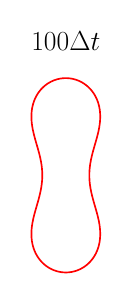
\begin{tikzpicture}[scale=0.4]

\begin{axis}[
  xmin = -1,
  xmax = 1,
  ymin = -2,
  ymax = 2,
  scale only axis,
  axis equal image,
  hide axis,
  title = {\Huge$100 \Delta t$}
  ]

\addplot [mark=none,red,line width=1.5] table{
4.1089e-01 -9.8874e-13
4.1097e-01 1.4110e-02
4.1122e-01 2.8854e-02
4.1169e-01 4.4499e-02
4.1238e-01 6.0790e-02
4.1328e-01 7.7035e-02
4.1433e-01 9.2399e-02
4.1544e-01 1.0635e-01
4.1661e-01 1.1932e-01
4.1800e-01 1.3318e-01
4.1992e-01 1.5023e-01
4.2267e-01 1.7192e-01
4.2656e-01 1.9886e-01
4.3188e-01 2.3102e-01
4.3879e-01 2.6779e-01
4.4733e-01 3.0810e-01
4.5729e-01 3.5063e-01
4.6829e-01 3.9393e-01
4.7980e-01 4.3657e-01
4.9127e-01 4.7738e-01
5.0223e-01 5.1546e-01
5.1233e-01 5.5028e-01
5.2141e-01 5.8170e-01
5.2949e-01 6.1002e-01
5.3674e-01 6.3591e-01
5.4338e-01 6.6020e-01
5.4960e-01 6.8367e-01
5.5554e-01 7.0684e-01
5.6126e-01 7.3016e-01
5.6685e-01 7.5412e-01
5.7242e-01 7.7953e-01
5.7807e-01 8.0740e-01
5.8378e-01 8.3876e-01
5.8936e-01 8.7427e-01
5.9439e-01 9.1418e-01
5.9829e-01 9.5817e-01
6.0040e-01 1.0055e+00
6.0010e-01 1.0548e+00
5.9699e-01 1.1048e+00
5.9100e-01 1.1536e+00
5.8240e-01 1.1999e+00
5.7175e-01 1.2425e+00
5.5971e-01 1.2810e+00
5.4683e-01 1.3153e+00
5.3342e-01 1.3461e+00
5.1944e-01 1.3743e+00
5.0461e-01 1.4010e+00
4.8867e-01 1.4267e+00
4.7151e-01 1.4516e+00
4.5322e-01 1.4756e+00
4.3401e-01 1.4984e+00
4.1402e-01 1.5199e+00
3.9309e-01 1.5404e+00
3.7071e-01 1.5601e+00
3.4611e-01 1.5797e+00
3.1860e-01 1.5993e+00
2.8779e-01 1.6185e+00
2.5378e-01 1.6367e+00
2.1719e-01 1.6533e+00
1.7904e-01 1.6674e+00
1.4059e-01 1.6787e+00
1.0302e-01 1.6869e+00
6.7102e-02 1.6923e+00
3.2969e-02 1.6953e+00
3.1565e-12 1.6963e+00
-3.2969e-02 1.6953e+00
-6.7102e-02 1.6923e+00
-1.0302e-01 1.6869e+00
-1.4059e-01 1.6787e+00
-1.7904e-01 1.6674e+00
-2.1719e-01 1.6533e+00
-2.5378e-01 1.6367e+00
-2.8779e-01 1.6185e+00
-3.1860e-01 1.5993e+00
-3.4611e-01 1.5797e+00
-3.7071e-01 1.5601e+00
-3.9309e-01 1.5404e+00
-4.1402e-01 1.5199e+00
-4.3401e-01 1.4984e+00
-4.5322e-01 1.4756e+00
-4.7151e-01 1.4516e+00
-4.8867e-01 1.4267e+00
-5.0461e-01 1.4010e+00
-5.1944e-01 1.3743e+00
-5.3342e-01 1.3461e+00
-5.4683e-01 1.3153e+00
-5.5971e-01 1.2810e+00
-5.7175e-01 1.2425e+00
-5.8240e-01 1.1999e+00
-5.9100e-01 1.1536e+00
-5.9699e-01 1.1048e+00
-6.0010e-01 1.0548e+00
-6.0040e-01 1.0055e+00
-5.9829e-01 9.5817e-01
-5.9439e-01 9.1418e-01
-5.8936e-01 8.7427e-01
-5.8378e-01 8.3876e-01
-5.7807e-01 8.0740e-01
-5.7242e-01 7.7953e-01
-5.6685e-01 7.5412e-01
-5.6126e-01 7.3016e-01
-5.5554e-01 7.0684e-01
-5.4960e-01 6.8367e-01
-5.4338e-01 6.6020e-01
-5.3674e-01 6.3591e-01
-5.2949e-01 6.1002e-01
-5.2141e-01 5.8170e-01
-5.1233e-01 5.5028e-01
-5.0223e-01 5.1546e-01
-4.9127e-01 4.7738e-01
-4.7980e-01 4.3657e-01
-4.6829e-01 3.9393e-01
-4.5729e-01 3.5063e-01
-4.4733e-01 3.0810e-01
-4.3879e-01 2.6779e-01
-4.3188e-01 2.3102e-01
-4.2656e-01 1.9886e-01
-4.2267e-01 1.7192e-01
-4.1992e-01 1.5023e-01
-4.1800e-01 1.3318e-01
-4.1661e-01 1.1932e-01
-4.1544e-01 1.0635e-01
-4.1433e-01 9.2399e-02
-4.1328e-01 7.7035e-02
-4.1238e-01 6.0790e-02
-4.1169e-01 4.4499e-02
-4.1122e-01 2.8854e-02
-4.1097e-01 1.4110e-02
-4.1089e-01 -1.4693e-11
-4.1097e-01 -1.4110e-02
-4.1122e-01 -2.8854e-02
-4.1169e-01 -4.4499e-02
-4.1238e-01 -6.0790e-02
-4.1328e-01 -7.7035e-02
-4.1433e-01 -9.2399e-02
-4.1544e-01 -1.0635e-01
-4.1661e-01 -1.1932e-01
-4.1800e-01 -1.3318e-01
-4.1992e-01 -1.5023e-01
-4.2267e-01 -1.7192e-01
-4.2656e-01 -1.9886e-01
-4.3188e-01 -2.3102e-01
-4.3879e-01 -2.6779e-01
-4.4733e-01 -3.0810e-01
-4.5729e-01 -3.5063e-01
-4.6829e-01 -3.9393e-01
-4.7980e-01 -4.3657e-01
-4.9127e-01 -4.7738e-01
-5.0223e-01 -5.1546e-01
-5.1233e-01 -5.5028e-01
-5.2141e-01 -5.8170e-01
-5.2949e-01 -6.1002e-01
-5.3674e-01 -6.3591e-01
-5.4338e-01 -6.6020e-01
-5.4960e-01 -6.8367e-01
-5.5554e-01 -7.0684e-01
-5.6126e-01 -7.3016e-01
-5.6685e-01 -7.5412e-01
-5.7242e-01 -7.7953e-01
-5.7807e-01 -8.0740e-01
-5.8378e-01 -8.3876e-01
-5.8936e-01 -8.7427e-01
-5.9439e-01 -9.1418e-01
-5.9829e-01 -9.5817e-01
-6.0040e-01 -1.0055e+00
-6.0010e-01 -1.0548e+00
-5.9699e-01 -1.1048e+00
-5.9100e-01 -1.1536e+00
-5.8240e-01 -1.1999e+00
-5.7175e-01 -1.2425e+00
-5.5971e-01 -1.2810e+00
-5.4683e-01 -1.3153e+00
-5.3342e-01 -1.3461e+00
-5.1944e-01 -1.3743e+00
-5.0461e-01 -1.4010e+00
-4.8867e-01 -1.4267e+00
-4.7151e-01 -1.4516e+00
-4.5322e-01 -1.4756e+00
-4.3401e-01 -1.4984e+00
-4.1402e-01 -1.5199e+00
-3.9309e-01 -1.5404e+00
-3.7071e-01 -1.5601e+00
-3.4611e-01 -1.5797e+00
-3.1860e-01 -1.5993e+00
-2.8779e-01 -1.6185e+00
-2.5378e-01 -1.6367e+00
-2.1719e-01 -1.6533e+00
-1.7904e-01 -1.6674e+00
-1.4059e-01 -1.6787e+00
-1.0302e-01 -1.6869e+00
-6.7102e-02 -1.6923e+00
-3.2969e-02 -1.6953e+00
2.7559e-12 -1.6963e+00
3.2969e-02 -1.6953e+00
6.7102e-02 -1.6923e+00
1.0302e-01 -1.6869e+00
1.4059e-01 -1.6787e+00
1.7904e-01 -1.6674e+00
2.1719e-01 -1.6533e+00
2.5378e-01 -1.6367e+00
2.8779e-01 -1.6185e+00
3.1860e-01 -1.5993e+00
3.4611e-01 -1.5797e+00
3.7071e-01 -1.5601e+00
3.9309e-01 -1.5404e+00
4.1402e-01 -1.5199e+00
4.3401e-01 -1.4984e+00
4.5322e-01 -1.4756e+00
4.7151e-01 -1.4516e+00
4.8867e-01 -1.4267e+00
5.0461e-01 -1.4010e+00
5.1944e-01 -1.3743e+00
5.3342e-01 -1.3461e+00
5.4683e-01 -1.3153e+00
5.5971e-01 -1.2810e+00
5.7175e-01 -1.2425e+00
5.8240e-01 -1.1999e+00
5.9100e-01 -1.1536e+00
5.9699e-01 -1.1048e+00
6.0010e-01 -1.0548e+00
6.0040e-01 -1.0055e+00
5.9829e-01 -9.5817e-01
5.9439e-01 -9.1418e-01
5.8936e-01 -8.7427e-01
5.8378e-01 -8.3876e-01
5.7807e-01 -8.0740e-01
5.7242e-01 -7.7953e-01
5.6685e-01 -7.5412e-01
5.6126e-01 -7.3016e-01
5.5554e-01 -7.0684e-01
5.4960e-01 -6.8367e-01
5.4338e-01 -6.6020e-01
5.3674e-01 -6.3591e-01
5.2949e-01 -6.1002e-01
5.2141e-01 -5.8170e-01
5.1233e-01 -5.5028e-01
5.0223e-01 -5.1546e-01
4.9127e-01 -4.7738e-01
4.7980e-01 -4.3657e-01
4.6829e-01 -3.9393e-01
4.5729e-01 -3.5063e-01
4.4733e-01 -3.0810e-01
4.3879e-01 -2.6779e-01
4.3188e-01 -2.3102e-01
4.2656e-01 -1.9886e-01
4.2267e-01 -1.7192e-01
4.1992e-01 -1.5023e-01
4.1800e-01 -1.3318e-01
4.1661e-01 -1.1932e-01
4.1544e-01 -1.0635e-01
4.1433e-01 -9.2399e-02
4.1328e-01 -7.7035e-02
4.1238e-01 -6.0790e-02
4.1169e-01 -4.4499e-02
4.1122e-01 -2.8854e-02
4.1097e-01 -1.4110e-02
4.1089e-01 -9.8874e-13
};


\end{axis}

\end{tikzpicture}



 &
    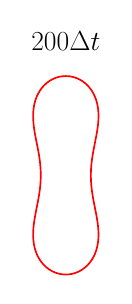
\begin{tikzpicture}[scale=0.4]

\begin{axis}[
  xmin = -1,
  xmax = 1,
  ymin = -2,
  ymax = 2,
  scale only axis,
  axis equal image,
  hide axis,
  title = {\Huge$200 \Delta t$}
  ]

\addplot [mark=none,red,line width=1.5] table{
4.3749e-01 1.4571e-12
4.3755e-01 1.4110e-02
4.3771e-01 2.8855e-02
4.3802e-01 4.4505e-02
4.3847e-01 6.0804e-02
4.3907e-01 7.7063e-02
4.3975e-01 9.2448e-02
4.4048e-01 1.0643e-01
4.4125e-01 1.1943e-01
4.4217e-01 1.3332e-01
4.4344e-01 1.5043e-01
4.4525e-01 1.7222e-01
4.4783e-01 1.9932e-01
4.5136e-01 2.3173e-01
4.5597e-01 2.6885e-01
4.6169e-01 3.0966e-01
4.6841e-01 3.5282e-01
4.7588e-01 3.9686e-01
4.8376e-01 4.4033e-01
4.9167e-01 4.8198e-01
4.9928e-01 5.2086e-01
5.0635e-01 5.5642e-01
5.1274e-01 5.8850e-01
5.1846e-01 6.1739e-01
5.2362e-01 6.4378e-01
5.2837e-01 6.6851e-01
5.3285e-01 6.9236e-01
5.3713e-01 7.1590e-01
5.4128e-01 7.3955e-01
5.4536e-01 7.6381e-01
5.4944e-01 7.8950e-01
5.5360e-01 8.1764e-01
5.5783e-01 8.4923e-01
5.6198e-01 8.8494e-01
5.6575e-01 9.2499e-01
5.6867e-01 9.6906e-01
5.7023e-01 1.0164e+00
5.6989e-01 1.0657e+00
5.6730e-01 1.1157e+00
5.6233e-01 1.1647e+00
5.5514e-01 1.2112e+00
5.4615e-01 1.2542e+00
5.3587e-01 1.2932e+00
5.2477e-01 1.3281e+00
5.1307e-01 1.3596e+00
5.0077e-01 1.3886e+00
4.8760e-01 1.4161e+00
4.7331e-01 1.4428e+00
4.5779e-01 1.4687e+00
4.4110e-01 1.4939e+00
4.2342e-01 1.5179e+00
4.0488e-01 1.5406e+00
3.8530e-01 1.5624e+00
3.6420e-01 1.5835e+00
3.4084e-01 1.6046e+00
3.1451e-01 1.6257e+00
2.8479e-01 1.6465e+00
2.5173e-01 1.6665e+00
2.1591e-01 1.6846e+00
1.7833e-01 1.7002e+00
1.4025e-01 1.7126e+00
1.0288e-01 1.7218e+00
6.7064e-02 1.7278e+00
3.2965e-02 1.7311e+00
-8.5061e-13 1.7322e+00
-3.2965e-02 1.7311e+00
-6.7064e-02 1.7278e+00
-1.0288e-01 1.7218e+00
-1.4025e-01 1.7126e+00
-1.7833e-01 1.7002e+00
-2.1591e-01 1.6846e+00
-2.5173e-01 1.6665e+00
-2.8479e-01 1.6465e+00
-3.1451e-01 1.6257e+00
-3.4084e-01 1.6046e+00
-3.6420e-01 1.5835e+00
-3.8530e-01 1.5624e+00
-4.0488e-01 1.5406e+00
-4.2342e-01 1.5179e+00
-4.4110e-01 1.4939e+00
-4.5779e-01 1.4687e+00
-4.7331e-01 1.4428e+00
-4.8760e-01 1.4161e+00
-5.0077e-01 1.3886e+00
-5.1307e-01 1.3596e+00
-5.2477e-01 1.3281e+00
-5.3587e-01 1.2932e+00
-5.4615e-01 1.2542e+00
-5.5514e-01 1.2112e+00
-5.6233e-01 1.1647e+00
-5.6730e-01 1.1157e+00
-5.6989e-01 1.0657e+00
-5.7023e-01 1.0164e+00
-5.6867e-01 9.6906e-01
-5.6575e-01 9.2499e-01
-5.6198e-01 8.8494e-01
-5.5783e-01 8.4923e-01
-5.5360e-01 8.1764e-01
-5.4944e-01 7.8950e-01
-5.4536e-01 7.6381e-01
-5.4128e-01 7.3955e-01
-5.3713e-01 7.1590e-01
-5.3285e-01 6.9236e-01
-5.2837e-01 6.6851e-01
-5.2362e-01 6.4378e-01
-5.1846e-01 6.1739e-01
-5.1274e-01 5.8850e-01
-5.0635e-01 5.5642e-01
-4.9928e-01 5.2086e-01
-4.9167e-01 4.8198e-01
-4.8376e-01 4.4033e-01
-4.7588e-01 3.9686e-01
-4.6841e-01 3.5282e-01
-4.6169e-01 3.0966e-01
-4.5597e-01 2.6885e-01
-4.5136e-01 2.3173e-01
-4.4783e-01 1.9932e-01
-4.4525e-01 1.7222e-01
-4.4344e-01 1.5043e-01
-4.4217e-01 1.3332e-01
-4.4125e-01 1.1943e-01
-4.4048e-01 1.0643e-01
-4.3975e-01 9.2448e-02
-4.3907e-01 7.7063e-02
-4.3847e-01 6.0804e-02
-4.3802e-01 4.4505e-02
-4.3771e-01 2.8855e-02
-4.3755e-01 1.4110e-02
-4.3749e-01 -1.7048e-11
-4.3755e-01 -1.4110e-02
-4.3771e-01 -2.8855e-02
-4.3802e-01 -4.4505e-02
-4.3847e-01 -6.0804e-02
-4.3907e-01 -7.7063e-02
-4.3975e-01 -9.2448e-02
-4.4048e-01 -1.0643e-01
-4.4125e-01 -1.1943e-01
-4.4217e-01 -1.3332e-01
-4.4344e-01 -1.5043e-01
-4.4525e-01 -1.7222e-01
-4.4783e-01 -1.9932e-01
-4.5136e-01 -2.3173e-01
-4.5597e-01 -2.6885e-01
-4.6169e-01 -3.0966e-01
-4.6841e-01 -3.5282e-01
-4.7588e-01 -3.9686e-01
-4.8376e-01 -4.4033e-01
-4.9167e-01 -4.8198e-01
-4.9928e-01 -5.2086e-01
-5.0635e-01 -5.5642e-01
-5.1274e-01 -5.8850e-01
-5.1846e-01 -6.1739e-01
-5.2362e-01 -6.4378e-01
-5.2837e-01 -6.6851e-01
-5.3285e-01 -6.9236e-01
-5.3713e-01 -7.1590e-01
-5.4128e-01 -7.3955e-01
-5.4536e-01 -7.6381e-01
-5.4944e-01 -7.8950e-01
-5.5360e-01 -8.1764e-01
-5.5783e-01 -8.4923e-01
-5.6198e-01 -8.8494e-01
-5.6575e-01 -9.2499e-01
-5.6867e-01 -9.6906e-01
-5.7023e-01 -1.0164e+00
-5.6989e-01 -1.0657e+00
-5.6730e-01 -1.1157e+00
-5.6233e-01 -1.1647e+00
-5.5514e-01 -1.2112e+00
-5.4615e-01 -1.2542e+00
-5.3587e-01 -1.2932e+00
-5.2477e-01 -1.3281e+00
-5.1307e-01 -1.3596e+00
-5.0077e-01 -1.3886e+00
-4.8760e-01 -1.4161e+00
-4.7331e-01 -1.4428e+00
-4.5779e-01 -1.4687e+00
-4.4110e-01 -1.4939e+00
-4.2342e-01 -1.5179e+00
-4.0488e-01 -1.5406e+00
-3.8530e-01 -1.5624e+00
-3.6420e-01 -1.5835e+00
-3.4084e-01 -1.6046e+00
-3.1451e-01 -1.6257e+00
-2.8479e-01 -1.6465e+00
-2.5173e-01 -1.6665e+00
-2.1591e-01 -1.6846e+00
-1.7833e-01 -1.7002e+00
-1.4025e-01 -1.7126e+00
-1.0288e-01 -1.7218e+00
-6.7064e-02 -1.7278e+00
-3.2965e-02 -1.7311e+00
-2.8432e-12 -1.7322e+00
3.2965e-02 -1.7311e+00
6.7064e-02 -1.7278e+00
1.0288e-01 -1.7218e+00
1.4025e-01 -1.7126e+00
1.7833e-01 -1.7002e+00
2.1591e-01 -1.6846e+00
2.5173e-01 -1.6665e+00
2.8479e-01 -1.6465e+00
3.1451e-01 -1.6257e+00
3.4084e-01 -1.6046e+00
3.6420e-01 -1.5835e+00
3.8530e-01 -1.5624e+00
4.0488e-01 -1.5406e+00
4.2342e-01 -1.5179e+00
4.4110e-01 -1.4939e+00
4.5779e-01 -1.4687e+00
4.7331e-01 -1.4428e+00
4.8760e-01 -1.4161e+00
5.0077e-01 -1.3886e+00
5.1307e-01 -1.3596e+00
5.2477e-01 -1.3281e+00
5.3587e-01 -1.2932e+00
5.4615e-01 -1.2542e+00
5.5514e-01 -1.2112e+00
5.6233e-01 -1.1647e+00
5.6730e-01 -1.1157e+00
5.6989e-01 -1.0657e+00
5.7023e-01 -1.0164e+00
5.6867e-01 -9.6906e-01
5.6575e-01 -9.2499e-01
5.6198e-01 -8.8494e-01
5.5783e-01 -8.4923e-01
5.5360e-01 -8.1764e-01
5.4944e-01 -7.8950e-01
5.4536e-01 -7.6381e-01
5.4128e-01 -7.3955e-01
5.3713e-01 -7.1590e-01
5.3285e-01 -6.9236e-01
5.2837e-01 -6.6851e-01
5.2362e-01 -6.4378e-01
5.1846e-01 -6.1739e-01
5.1274e-01 -5.8850e-01
5.0635e-01 -5.5642e-01
4.9928e-01 -5.2086e-01
4.9167e-01 -4.8198e-01
4.8376e-01 -4.4033e-01
4.7588e-01 -3.9686e-01
4.6841e-01 -3.5282e-01
4.6169e-01 -3.0966e-01
4.5597e-01 -2.6885e-01
4.5136e-01 -2.3173e-01
4.4783e-01 -1.9932e-01
4.4525e-01 -1.7222e-01
4.4344e-01 -1.5043e-01
4.4217e-01 -1.3332e-01
4.4125e-01 -1.1943e-01
4.4048e-01 -1.0643e-01
4.3975e-01 -9.2448e-02
4.3907e-01 -7.7063e-02
4.3847e-01 -6.0804e-02
4.3802e-01 -4.4505e-02
4.3771e-01 -2.8855e-02
4.3755e-01 -1.4110e-02
4.3749e-01 1.4571e-12
};


\end{axis}

\end{tikzpicture}



 &
    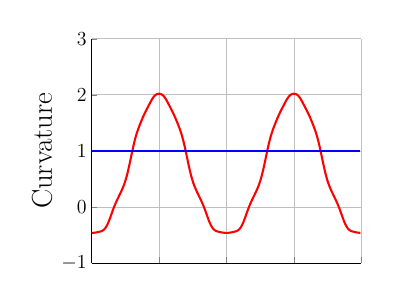
\begin{tikzpicture}[scale=0.5]

\begin{axis}[
  xmin = 0,
  xmax = 6.2832,
  ymin = -1,
  ymax = 3,
  xtick = {0,1.5708,3.1416,4.7124,6.2832},
  xticklabels = {},
  ytick = {-1,0,1,2,3},
  yticklabels = {\Large$-1$,\Large$0$,\Large$1$,\Large$2$,\Large$3$},
  ylabel = {\huge Curvature},
  axis y line* = left,
  axis x line* = bottom,
  grid,
%  legend entries = {$\kappa$,$\tilde{\kappa}$},
%  legend style={at={(0.6,1.1)}, anchor=north west},
%  label style = {draw=none,font=\small},
%  legend cell align = left, 
  ]

\addplot [mark=none,red,line width=1.5] table{
0.0000e+00 -4.6484e-01
2.4544e-02 -4.6363e-01
4.9087e-02 -4.6346e-01
7.3631e-02 -4.6095e-01
9.8175e-02 -4.5890e-01
1.2272e-01 -4.5483e-01
1.4726e-01 -4.5133e-01
1.7181e-01 -4.4646e-01
1.9635e-01 -4.4238e-01
2.2089e-01 -4.3659e-01
2.4544e-01 -4.2932e-01
2.6998e-01 -4.1831e-01
2.9452e-01 -4.0302e-01
3.1907e-01 -3.8162e-01
3.4361e-01 -3.5371e-01
3.6816e-01 -3.1842e-01
3.9270e-01 -2.7656e-01
4.1724e-01 -2.2885e-01
4.4179e-01 -1.7757e-01
4.6633e-01 -1.2436e-01
4.9087e-01 -7.1828e-02
5.1542e-01 -2.1066e-02
5.3996e-01 2.6173e-02
5.6450e-01 7.0509e-02
5.8905e-01 1.1151e-01
6.1359e-01 1.5132e-01
6.3814e-01 1.8980e-01
6.6268e-01 2.2897e-01
6.8722e-01 2.6830e-01
7.1177e-01 3.0969e-01
7.3631e-01 3.5357e-01
7.6085e-01 4.0253e-01
7.8540e-01 4.5778e-01
8.0994e-01 5.2102e-01
8.3449e-01 5.9241e-01
8.5903e-01 6.7155e-01
8.8357e-01 7.5688e-01
9.0812e-01 8.4611e-01
9.3266e-01 9.3643e-01
9.5720e-01 1.0247e+00
9.8175e-01 1.1085e+00
1.0063e+00 1.1855e+00
1.0308e+00 1.2552e+00
1.0554e+00 1.3171e+00
1.0799e+00 1.3731e+00
1.1045e+00 1.4240e+00
1.1290e+00 1.4728e+00
1.1536e+00 1.5191e+00
1.1781e+00 1.5650e+00
1.2026e+00 1.6083e+00
1.2272e+00 1.6505e+00
1.2517e+00 1.6894e+00
1.2763e+00 1.7276e+00
1.3008e+00 1.7634e+00
1.3254e+00 1.8002e+00
1.3499e+00 1.8359e+00
1.3744e+00 1.8721e+00
1.3990e+00 1.9057e+00
1.4235e+00 1.9372e+00
1.4481e+00 1.9632e+00
1.4726e+00 1.9848e+00
1.4972e+00 1.9999e+00
1.5217e+00 2.0107e+00
1.5463e+00 2.0157e+00
1.5708e+00 2.0182e+00
1.5953e+00 2.0157e+00
1.6199e+00 2.0107e+00
1.6444e+00 1.9999e+00
1.6690e+00 1.9848e+00
1.6935e+00 1.9632e+00
1.7181e+00 1.9372e+00
1.7426e+00 1.9057e+00
1.7671e+00 1.8721e+00
1.7917e+00 1.8359e+00
1.8162e+00 1.8002e+00
1.8408e+00 1.7634e+00
1.8653e+00 1.7276e+00
1.8899e+00 1.6894e+00
1.9144e+00 1.6505e+00
1.9390e+00 1.6083e+00
1.9635e+00 1.5650e+00
1.9880e+00 1.5191e+00
2.0126e+00 1.4728e+00
2.0371e+00 1.4240e+00
2.0617e+00 1.3731e+00
2.0862e+00 1.3171e+00
2.1108e+00 1.2552e+00
2.1353e+00 1.1855e+00
2.1598e+00 1.1085e+00
2.1844e+00 1.0247e+00
2.2089e+00 9.3643e-01
2.2335e+00 8.4611e-01
2.2580e+00 7.5688e-01
2.2826e+00 6.7155e-01
2.3071e+00 5.9241e-01
2.3317e+00 5.2102e-01
2.3562e+00 4.5778e-01
2.3807e+00 4.0253e-01
2.4053e+00 3.5357e-01
2.4298e+00 3.0969e-01
2.4544e+00 2.6830e-01
2.4789e+00 2.2897e-01
2.5035e+00 1.8980e-01
2.5280e+00 1.5132e-01
2.5525e+00 1.1151e-01
2.5771e+00 7.0509e-02
2.6016e+00 2.6173e-02
2.6262e+00 -2.1066e-02
2.6507e+00 -7.1828e-02
2.6753e+00 -1.2436e-01
2.6998e+00 -1.7757e-01
2.7243e+00 -2.2885e-01
2.7489e+00 -2.7656e-01
2.7734e+00 -3.1842e-01
2.7980e+00 -3.5371e-01
2.8225e+00 -3.8162e-01
2.8471e+00 -4.0302e-01
2.8716e+00 -4.1831e-01
2.8962e+00 -4.2932e-01
2.9207e+00 -4.3659e-01
2.9452e+00 -4.4238e-01
2.9698e+00 -4.4646e-01
2.9943e+00 -4.5133e-01
3.0189e+00 -4.5483e-01
3.0434e+00 -4.5891e-01
3.0680e+00 -4.6095e-01
3.0925e+00 -4.6346e-01
3.1170e+00 -4.6363e-01
3.1416e+00 -4.6484e-01
3.1661e+00 -4.6363e-01
3.1907e+00 -4.6346e-01
3.2152e+00 -4.6095e-01
3.2398e+00 -4.5891e-01
3.2643e+00 -4.5483e-01
3.2889e+00 -4.5133e-01
3.3134e+00 -4.4646e-01
3.3379e+00 -4.4238e-01
3.3625e+00 -4.3659e-01
3.3870e+00 -4.2932e-01
3.4116e+00 -4.1831e-01
3.4361e+00 -4.0302e-01
3.4607e+00 -3.8162e-01
3.4852e+00 -3.5371e-01
3.5097e+00 -3.1842e-01
3.5343e+00 -2.7656e-01
3.5588e+00 -2.2885e-01
3.5834e+00 -1.7757e-01
3.6079e+00 -1.2436e-01
3.6325e+00 -7.1828e-02
3.6570e+00 -2.1066e-02
3.6816e+00 2.6173e-02
3.7061e+00 7.0509e-02
3.7306e+00 1.1151e-01
3.7552e+00 1.5132e-01
3.7797e+00 1.8980e-01
3.8043e+00 2.2897e-01
3.8288e+00 2.6830e-01
3.8534e+00 3.0969e-01
3.8779e+00 3.5357e-01
3.9024e+00 4.0253e-01
3.9270e+00 4.5778e-01
3.9515e+00 5.2102e-01
3.9761e+00 5.9241e-01
4.0006e+00 6.7155e-01
4.0252e+00 7.5688e-01
4.0497e+00 8.4611e-01
4.0743e+00 9.3643e-01
4.0988e+00 1.0247e+00
4.1233e+00 1.1085e+00
4.1479e+00 1.1855e+00
4.1724e+00 1.2552e+00
4.1970e+00 1.3171e+00
4.2215e+00 1.3731e+00
4.2461e+00 1.4240e+00
4.2706e+00 1.4728e+00
4.2951e+00 1.5191e+00
4.3197e+00 1.5650e+00
4.3442e+00 1.6083e+00
4.3688e+00 1.6505e+00
4.3933e+00 1.6894e+00
4.4179e+00 1.7276e+00
4.4424e+00 1.7634e+00
4.4670e+00 1.8002e+00
4.4915e+00 1.8359e+00
4.5160e+00 1.8721e+00
4.5406e+00 1.9057e+00
4.5651e+00 1.9372e+00
4.5897e+00 1.9632e+00
4.6142e+00 1.9848e+00
4.6388e+00 1.9999e+00
4.6633e+00 2.0107e+00
4.6878e+00 2.0157e+00
4.7124e+00 2.0182e+00
4.7369e+00 2.0157e+00
4.7615e+00 2.0107e+00
4.7860e+00 1.9999e+00
4.8106e+00 1.9848e+00
4.8351e+00 1.9632e+00
4.8597e+00 1.9372e+00
4.8842e+00 1.9057e+00
4.9087e+00 1.8721e+00
4.9333e+00 1.8359e+00
4.9578e+00 1.8002e+00
4.9824e+00 1.7634e+00
5.0069e+00 1.7276e+00
5.0315e+00 1.6894e+00
5.0560e+00 1.6505e+00
5.0805e+00 1.6083e+00
5.1051e+00 1.5650e+00
5.1296e+00 1.5191e+00
5.1542e+00 1.4728e+00
5.1787e+00 1.4240e+00
5.2033e+00 1.3731e+00
5.2278e+00 1.3171e+00
5.2524e+00 1.2552e+00
5.2769e+00 1.1855e+00
5.3014e+00 1.1085e+00
5.3260e+00 1.0247e+00
5.3505e+00 9.3643e-01
5.3751e+00 8.4611e-01
5.3996e+00 7.5688e-01
5.4242e+00 6.7155e-01
5.4487e+00 5.9241e-01
5.4732e+00 5.2102e-01
5.4978e+00 4.5778e-01
5.5223e+00 4.0253e-01
5.5469e+00 3.5357e-01
5.5714e+00 3.0969e-01
5.5960e+00 2.6830e-01
5.6205e+00 2.2897e-01
5.6450e+00 1.8980e-01
5.6696e+00 1.5132e-01
5.6941e+00 1.1151e-01
5.7187e+00 7.0509e-02
5.7432e+00 2.6173e-02
5.7678e+00 -2.1066e-02
5.7923e+00 -7.1828e-02
5.8169e+00 -1.2436e-01
5.8414e+00 -1.7757e-01
5.8659e+00 -2.2885e-01
5.8905e+00 -2.7656e-01
5.9150e+00 -3.1842e-01
5.9396e+00 -3.5371e-01
5.9641e+00 -3.8162e-01
5.9887e+00 -4.0302e-01
6.0132e+00 -4.1831e-01
6.0377e+00 -4.2932e-01
6.0623e+00 -4.3659e-01
6.0868e+00 -4.4238e-01
6.1114e+00 -4.4646e-01
6.1359e+00 -4.5133e-01
6.1605e+00 -4.5483e-01
6.1850e+00 -4.5890e-01
6.2096e+00 -4.6095e-01
6.2341e+00 -4.6346e-01
6.2586e+00 -4.6363e-01
};

\addplot [mark=none,blue,line width=1.5] table{
0.0000e+00 1.0000e+00
2.4544e-02 1.0000e+00
4.9087e-02 1.0000e+00
7.3631e-02 1.0000e+00
9.8175e-02 1.0000e+00
1.2272e-01 1.0000e+00
1.4726e-01 1.0000e+00
1.7181e-01 1.0000e+00
1.9635e-01 1.0000e+00
2.2089e-01 1.0000e+00
2.4544e-01 1.0000e+00
2.6998e-01 1.0000e+00
2.9452e-01 1.0000e+00
3.1907e-01 1.0000e+00
3.4361e-01 1.0000e+00
3.6816e-01 1.0000e+00
3.9270e-01 1.0000e+00
4.1724e-01 1.0000e+00
4.4179e-01 1.0000e+00
4.6633e-01 1.0000e+00
4.9087e-01 1.0000e+00
5.1542e-01 1.0000e+00
5.3996e-01 1.0000e+00
5.6450e-01 1.0000e+00
5.8905e-01 1.0000e+00
6.1359e-01 1.0000e+00
6.3814e-01 1.0000e+00
6.6268e-01 1.0000e+00
6.8722e-01 1.0000e+00
7.1177e-01 1.0000e+00
7.3631e-01 1.0000e+00
7.6085e-01 1.0000e+00
7.8540e-01 1.0000e+00
8.0994e-01 1.0000e+00
8.3449e-01 1.0000e+00
8.5903e-01 1.0000e+00
8.8357e-01 1.0000e+00
9.0812e-01 1.0000e+00
9.3266e-01 1.0000e+00
9.5720e-01 1.0000e+00
9.8175e-01 1.0000e+00
1.0063e+00 1.0000e+00
1.0308e+00 1.0000e+00
1.0554e+00 1.0000e+00
1.0799e+00 1.0000e+00
1.1045e+00 1.0000e+00
1.1290e+00 1.0000e+00
1.1536e+00 1.0000e+00
1.1781e+00 1.0000e+00
1.2026e+00 1.0000e+00
1.2272e+00 1.0000e+00
1.2517e+00 1.0000e+00
1.2763e+00 1.0000e+00
1.3008e+00 1.0000e+00
1.3254e+00 1.0000e+00
1.3499e+00 1.0000e+00
1.3744e+00 1.0000e+00
1.3990e+00 1.0000e+00
1.4235e+00 1.0000e+00
1.4481e+00 1.0000e+00
1.4726e+00 1.0000e+00
1.4972e+00 1.0000e+00
1.5217e+00 1.0000e+00
1.5463e+00 1.0000e+00
1.5708e+00 1.0000e+00
1.5953e+00 1.0000e+00
1.6199e+00 1.0000e+00
1.6444e+00 1.0000e+00
1.6690e+00 1.0000e+00
1.6935e+00 1.0000e+00
1.7181e+00 1.0000e+00
1.7426e+00 1.0000e+00
1.7671e+00 1.0000e+00
1.7917e+00 1.0000e+00
1.8162e+00 1.0000e+00
1.8408e+00 1.0000e+00
1.8653e+00 1.0000e+00
1.8899e+00 1.0000e+00
1.9144e+00 1.0000e+00
1.9390e+00 1.0000e+00
1.9635e+00 1.0000e+00
1.9880e+00 1.0000e+00
2.0126e+00 1.0000e+00
2.0371e+00 1.0000e+00
2.0617e+00 1.0000e+00
2.0862e+00 1.0000e+00
2.1108e+00 1.0000e+00
2.1353e+00 1.0000e+00
2.1598e+00 1.0000e+00
2.1844e+00 1.0000e+00
2.2089e+00 1.0000e+00
2.2335e+00 1.0000e+00
2.2580e+00 1.0000e+00
2.2826e+00 1.0000e+00
2.3071e+00 1.0000e+00
2.3317e+00 1.0000e+00
2.3562e+00 1.0000e+00
2.3807e+00 1.0000e+00
2.4053e+00 1.0000e+00
2.4298e+00 1.0000e+00
2.4544e+00 1.0000e+00
2.4789e+00 1.0000e+00
2.5035e+00 1.0000e+00
2.5280e+00 1.0000e+00
2.5525e+00 1.0000e+00
2.5771e+00 1.0000e+00
2.6016e+00 1.0000e+00
2.6262e+00 1.0000e+00
2.6507e+00 1.0000e+00
2.6753e+00 1.0000e+00
2.6998e+00 1.0000e+00
2.7243e+00 1.0000e+00
2.7489e+00 1.0000e+00
2.7734e+00 1.0000e+00
2.7980e+00 1.0000e+00
2.8225e+00 1.0000e+00
2.8471e+00 1.0000e+00
2.8716e+00 1.0000e+00
2.8962e+00 1.0000e+00
2.9207e+00 1.0000e+00
2.9452e+00 1.0000e+00
2.9698e+00 1.0000e+00
2.9943e+00 1.0000e+00
3.0189e+00 1.0000e+00
3.0434e+00 1.0000e+00
3.0680e+00 1.0000e+00
3.0925e+00 1.0000e+00
3.1170e+00 1.0000e+00
3.1416e+00 1.0000e+00
3.1661e+00 1.0000e+00
3.1907e+00 1.0000e+00
3.2152e+00 1.0000e+00
3.2398e+00 1.0000e+00
3.2643e+00 1.0000e+00
3.2889e+00 1.0000e+00
3.3134e+00 1.0000e+00
3.3379e+00 1.0000e+00
3.3625e+00 1.0000e+00
3.3870e+00 1.0000e+00
3.4116e+00 1.0000e+00
3.4361e+00 1.0000e+00
3.4607e+00 1.0000e+00
3.4852e+00 1.0000e+00
3.5097e+00 1.0000e+00
3.5343e+00 1.0000e+00
3.5588e+00 1.0000e+00
3.5834e+00 1.0000e+00
3.6079e+00 1.0000e+00
3.6325e+00 1.0000e+00
3.6570e+00 1.0000e+00
3.6816e+00 1.0000e+00
3.7061e+00 1.0000e+00
3.7306e+00 1.0000e+00
3.7552e+00 1.0000e+00
3.7797e+00 1.0000e+00
3.8043e+00 1.0000e+00
3.8288e+00 1.0000e+00
3.8534e+00 1.0000e+00
3.8779e+00 1.0000e+00
3.9024e+00 1.0000e+00
3.9270e+00 1.0000e+00
3.9515e+00 1.0000e+00
3.9761e+00 1.0000e+00
4.0006e+00 1.0000e+00
4.0252e+00 1.0000e+00
4.0497e+00 1.0000e+00
4.0743e+00 1.0000e+00
4.0988e+00 1.0000e+00
4.1233e+00 1.0000e+00
4.1479e+00 1.0000e+00
4.1724e+00 1.0000e+00
4.1970e+00 1.0000e+00
4.2215e+00 1.0000e+00
4.2461e+00 1.0000e+00
4.2706e+00 1.0000e+00
4.2951e+00 1.0000e+00
4.3197e+00 1.0000e+00
4.3442e+00 1.0000e+00
4.3688e+00 1.0000e+00
4.3933e+00 1.0000e+00
4.4179e+00 1.0000e+00
4.4424e+00 1.0000e+00
4.4670e+00 1.0000e+00
4.4915e+00 1.0000e+00
4.5160e+00 1.0000e+00
4.5406e+00 1.0000e+00
4.5651e+00 1.0000e+00
4.5897e+00 1.0000e+00
4.6142e+00 1.0000e+00
4.6388e+00 1.0000e+00
4.6633e+00 1.0000e+00
4.6878e+00 1.0000e+00
4.7124e+00 1.0000e+00
4.7369e+00 1.0000e+00
4.7615e+00 1.0000e+00
4.7860e+00 1.0000e+00
4.8106e+00 1.0000e+00
4.8351e+00 1.0000e+00
4.8597e+00 1.0000e+00
4.8842e+00 1.0000e+00
4.9087e+00 1.0000e+00
4.9333e+00 1.0000e+00
4.9578e+00 1.0000e+00
4.9824e+00 1.0000e+00
5.0069e+00 1.0000e+00
5.0315e+00 1.0000e+00
5.0560e+00 1.0000e+00
5.0805e+00 1.0000e+00
5.1051e+00 1.0000e+00
5.1296e+00 1.0000e+00
5.1542e+00 1.0000e+00
5.1787e+00 1.0000e+00
5.2033e+00 1.0000e+00
5.2278e+00 1.0000e+00
5.2524e+00 1.0000e+00
5.2769e+00 1.0000e+00
5.3014e+00 1.0000e+00
5.3260e+00 1.0000e+00
5.3505e+00 1.0000e+00
5.3751e+00 1.0000e+00
5.3996e+00 1.0000e+00
5.4242e+00 1.0000e+00
5.4487e+00 1.0000e+00
5.4732e+00 1.0000e+00
5.4978e+00 1.0000e+00
5.5223e+00 1.0000e+00
5.5469e+00 1.0000e+00
5.5714e+00 1.0000e+00
5.5960e+00 1.0000e+00
5.6205e+00 1.0000e+00
5.6450e+00 1.0000e+00
5.6696e+00 1.0000e+00
5.6941e+00 1.0000e+00
5.7187e+00 1.0000e+00
5.7432e+00 1.0000e+00
5.7678e+00 1.0000e+00
5.7923e+00 1.0000e+00
5.8169e+00 1.0000e+00
5.8414e+00 1.0000e+00
5.8659e+00 1.0000e+00
5.8905e+00 1.0000e+00
5.9150e+00 1.0000e+00
5.9396e+00 1.0000e+00
5.9641e+00 1.0000e+00
5.9887e+00 1.0000e+00
6.0132e+00 1.0000e+00
6.0377e+00 1.0000e+00
6.0623e+00 1.0000e+00
6.0868e+00 1.0000e+00
6.1114e+00 1.0000e+00
6.1359e+00 1.0000e+00
6.1605e+00 1.0000e+00
6.1850e+00 1.0000e+00
6.2096e+00 1.0000e+00
6.2341e+00 1.0000e+00
6.2586e+00 1.0000e+00
};

\end{axis}

\end{tikzpicture}



 \\

    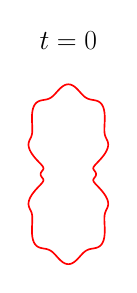
\begin{tikzpicture}[scale=0.4]

\begin{axis}[
  xmin = -1,
  xmax = 1,
  ymin = -2,
  ymax = 2,
  scale only axis,
  axis equal image,
  hide axis,
  title = {\Huge$t=0$}
  ]

\addplot [mark=none,red,line width=1.5] table{
4.8450e-01 0.0000e+00
4.8282e-01 1.3944e-02
4.7797e-01 2.7625e-02
4.7057e-01 4.0837e-02
4.6157e-01 5.3483e-02
4.5216e-01 6.5610e-02
4.4368e-01 7.7429e-02
4.3749e-01 8.9309e-02
4.3482e-01 1.0175e-01
4.3664e-01 1.1536e-01
4.4363e-01 1.3073e-01
4.5602e-01 1.4847e-01
4.7362e-01 1.6902e-01
4.9581e-01 1.9270e-01
5.2161e-01 2.1957e-01
5.4970e-01 2.4946e-01
5.7862e-01 2.8197e-01
6.0680e-01 3.1644e-01
6.3277e-01 3.5209e-01
6.5522e-01 3.8801e-01
6.7317e-01 4.2331e-01
6.8596e-01 4.5717e-01
6.9337e-01 4.8893e-01
6.9559e-01 5.1821e-01
6.9318e-01 5.4490e-01
6.8700e-01 5.6922e-01
6.7816e-01 5.9171e-01
6.6784e-01 6.1317e-01
6.5726e-01 6.3458e-01
6.4746e-01 6.5706e-01
6.3932e-01 6.8170e-01
6.3339e-01 7.0946e-01
6.2991e-01 7.4107e-01
6.2877e-01 7.7696e-01
6.2953e-01 8.1715e-01
6.3150e-01 8.6127e-01
6.3378e-01 9.0854e-01
6.3539e-01 9.5785e-01
6.3533e-01 1.0078e+00
6.3270e-01 1.0569e+00
6.2678e-01 1.1036e+00
6.1707e-01 1.1464e+00
6.0334e-01 1.1842e+00
5.8565e-01 1.2163e+00
5.6432e-01 1.2421e+00
5.3988e-01 1.2618e+00
5.1301e-01 1.2761e+00
4.8448e-01 1.2859e+00
4.5506e-01 1.2925e+00
4.2543e-01 1.2975e+00
3.9616e-01 1.3026e+00
3.6763e-01 1.3092e+00
3.4002e-01 1.3187e+00
3.1334e-01 1.3321e+00
2.8738e-01 1.3498e+00
2.6183e-01 1.3718e+00
2.3629e-01 1.3975e+00
2.1033e-01 1.4261e+00
1.8358e-01 1.4560e+00
1.5574e-01 1.4856e+00
1.2667e-01 1.5130e+00
9.6346e-02 1.5366e+00
6.4922e-02 1.5547e+00
3.2679e-02 1.5661e+00
8.1715e-17 1.5700e+00
-3.2679e-02 1.5661e+00
-6.4922e-02 1.5547e+00
-9.6346e-02 1.5366e+00
-1.2667e-01 1.5130e+00
-1.5574e-01 1.4856e+00
-1.8358e-01 1.4560e+00
-2.1033e-01 1.4261e+00
-2.3629e-01 1.3975e+00
-2.6183e-01 1.3718e+00
-2.8738e-01 1.3498e+00
-3.1334e-01 1.3321e+00
-3.4002e-01 1.3187e+00
-3.6763e-01 1.3092e+00
-3.9616e-01 1.3026e+00
-4.2543e-01 1.2975e+00
-4.5506e-01 1.2925e+00
-4.8448e-01 1.2859e+00
-5.1301e-01 1.2761e+00
-5.3988e-01 1.2618e+00
-5.6432e-01 1.2421e+00
-5.8565e-01 1.2163e+00
-6.0334e-01 1.1842e+00
-6.1707e-01 1.1464e+00
-6.2678e-01 1.1036e+00
-6.3270e-01 1.0569e+00
-6.3533e-01 1.0078e+00
-6.3539e-01 9.5785e-01
-6.3378e-01 9.0854e-01
-6.3150e-01 8.6127e-01
-6.2953e-01 8.1715e-01
-6.2877e-01 7.7696e-01
-6.2991e-01 7.4107e-01
-6.3339e-01 7.0946e-01
-6.3932e-01 6.8170e-01
-6.4746e-01 6.5706e-01
-6.5726e-01 6.3458e-01
-6.6784e-01 6.1317e-01
-6.7816e-01 5.9171e-01
-6.8700e-01 5.6922e-01
-6.9318e-01 5.4490e-01
-6.9559e-01 5.1821e-01
-6.9337e-01 4.8893e-01
-6.8596e-01 4.5717e-01
-6.7317e-01 4.2331e-01
-6.5522e-01 3.8801e-01
-6.3277e-01 3.5209e-01
-6.0680e-01 3.1644e-01
-5.7862e-01 2.8197e-01
-5.4970e-01 2.4946e-01
-5.2161e-01 2.1957e-01
-4.9581e-01 1.9270e-01
-4.7362e-01 1.6902e-01
-4.5602e-01 1.4847e-01
-4.4363e-01 1.3073e-01
-4.3664e-01 1.1536e-01
-4.3482e-01 1.0175e-01
-4.3749e-01 8.9309e-02
-4.4368e-01 7.7429e-02
-4.5216e-01 6.5610e-02
-4.6157e-01 5.3483e-02
-4.7057e-01 4.0837e-02
-4.7797e-01 2.7625e-02
-4.8282e-01 1.3944e-02
-4.8450e-01 6.9805e-17
-4.8282e-01 -1.3944e-02
-4.7797e-01 -2.7625e-02
-4.7057e-01 -4.0837e-02
-4.6157e-01 -5.3483e-02
-4.5216e-01 -6.5610e-02
-4.4368e-01 -7.7429e-02
-4.3749e-01 -8.9309e-02
-4.3482e-01 -1.0175e-01
-4.3664e-01 -1.1536e-01
-4.4363e-01 -1.3073e-01
-4.5602e-01 -1.4847e-01
-4.7362e-01 -1.6902e-01
-4.9581e-01 -1.9270e-01
-5.2161e-01 -2.1957e-01
-5.4970e-01 -2.4946e-01
-5.7862e-01 -2.8197e-01
-6.0680e-01 -3.1644e-01
-6.3277e-01 -3.5209e-01
-6.5522e-01 -3.8801e-01
-6.7317e-01 -4.2331e-01
-6.8596e-01 -4.5717e-01
-6.9337e-01 -4.8893e-01
-6.9559e-01 -5.1821e-01
-6.9318e-01 -5.4490e-01
-6.8700e-01 -5.6922e-01
-6.7816e-01 -5.9171e-01
-6.6784e-01 -6.1317e-01
-6.5726e-01 -6.3458e-01
-6.4746e-01 -6.5706e-01
-6.3932e-01 -6.8170e-01
-6.3339e-01 -7.0946e-01
-6.2991e-01 -7.4107e-01
-6.2877e-01 -7.7696e-01
-6.2953e-01 -8.1715e-01
-6.3150e-01 -8.6127e-01
-6.3378e-01 -9.0854e-01
-6.3539e-01 -9.5785e-01
-6.3533e-01 -1.0078e+00
-6.3270e-01 -1.0569e+00
-6.2678e-01 -1.1036e+00
-6.1707e-01 -1.1464e+00
-6.0334e-01 -1.1842e+00
-5.8565e-01 -1.2163e+00
-5.6432e-01 -1.2421e+00
-5.3988e-01 -1.2618e+00
-5.1301e-01 -1.2761e+00
-4.8448e-01 -1.2859e+00
-4.5506e-01 -1.2925e+00
-4.2543e-01 -1.2975e+00
-3.9616e-01 -1.3026e+00
-3.6763e-01 -1.3092e+00
-3.4002e-01 -1.3187e+00
-3.1334e-01 -1.3321e+00
-2.8738e-01 -1.3498e+00
-2.6183e-01 -1.3718e+00
-2.3629e-01 -1.3975e+00
-2.1033e-01 -1.4261e+00
-1.8358e-01 -1.4560e+00
-1.5574e-01 -1.4856e+00
-1.2667e-01 -1.5130e+00
-9.6346e-02 -1.5366e+00
-6.4922e-02 -1.5547e+00
-3.2679e-02 -1.5661e+00
-2.4514e-16 -1.5700e+00
3.2679e-02 -1.5661e+00
6.4922e-02 -1.5547e+00
9.6346e-02 -1.5366e+00
1.2667e-01 -1.5130e+00
1.5574e-01 -1.4856e+00
1.8358e-01 -1.4560e+00
2.1033e-01 -1.4261e+00
2.3629e-01 -1.3975e+00
2.6183e-01 -1.3718e+00
2.8738e-01 -1.3498e+00
3.1334e-01 -1.3321e+00
3.4002e-01 -1.3187e+00
3.6763e-01 -1.3092e+00
3.9616e-01 -1.3026e+00
4.2543e-01 -1.2975e+00
4.5506e-01 -1.2925e+00
4.8448e-01 -1.2859e+00
5.1301e-01 -1.2761e+00
5.3988e-01 -1.2618e+00
5.6432e-01 -1.2421e+00
5.8565e-01 -1.2163e+00
6.0334e-01 -1.1842e+00
6.1707e-01 -1.1464e+00
6.2678e-01 -1.1036e+00
6.3270e-01 -1.0569e+00
6.3533e-01 -1.0078e+00
6.3539e-01 -9.5785e-01
6.3378e-01 -9.0854e-01
6.3150e-01 -8.6127e-01
6.2953e-01 -8.1715e-01
6.2877e-01 -7.7696e-01
6.2991e-01 -7.4107e-01
6.3339e-01 -7.0946e-01
6.3932e-01 -6.8170e-01
6.4746e-01 -6.5706e-01
6.5726e-01 -6.3458e-01
6.6784e-01 -6.1317e-01
6.7816e-01 -5.9171e-01
6.8700e-01 -5.6922e-01
6.9318e-01 -5.4490e-01
6.9559e-01 -5.1821e-01
6.9337e-01 -4.8893e-01
6.8596e-01 -4.5717e-01
6.7317e-01 -4.2331e-01
6.5522e-01 -3.8801e-01
6.3277e-01 -3.5209e-01
6.0680e-01 -3.1644e-01
5.7862e-01 -2.8197e-01
5.4970e-01 -2.4946e-01
5.2161e-01 -2.1957e-01
4.9581e-01 -1.9270e-01
4.7362e-01 -1.6902e-01
4.5602e-01 -1.4847e-01
4.4363e-01 -1.3073e-01
4.3664e-01 -1.1536e-01
4.3482e-01 -1.0175e-01
4.3749e-01 -8.9309e-02
4.4368e-01 -7.7429e-02
4.5216e-01 -6.5610e-02
4.6157e-01 -5.3483e-02
4.7057e-01 -4.0837e-02
4.7797e-01 -2.7625e-02
4.8282e-01 -1.3944e-02
4.8450e-01 0.0000e+00
};


\end{axis}

\end{tikzpicture}



 &
    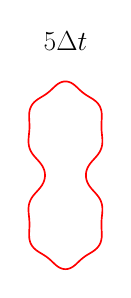
\begin{tikzpicture}[scale=0.4]

\begin{axis}[
  xmin = -1,
  xmax = 1,
  ymin = -2,
  ymax = 2,
  scale only axis,
  axis equal image,
  hide axis,
  title = {\Huge$5\Delta t$}
  ]

\addplot [mark=none,red,line width=1.5] table{
3.5726e-01 -4.9433e-12
3.5760e-01 1.4105e-02
3.5867e-01 2.8811e-02
3.6060e-01 4.4342e-02
3.6346e-01 6.0391e-02
3.6717e-01 7.6229e-02
3.7144e-01 9.1022e-02
3.7594e-01 1.0427e-01
3.8063e-01 1.1642e-01
3.8616e-01 1.2919e-01
3.9367e-01 1.4461e-01
4.0426e-01 1.6373e-01
4.1886e-01 1.8669e-01
4.3807e-01 2.1300e-01
4.6183e-01 2.4187e-01
4.8929e-01 2.7256e-01
5.1881e-01 3.0473e-01
5.4820e-01 3.3834e-01
5.7520e-01 3.7328e-01
5.9800e-01 4.0898e-01
6.1568e-01 4.4442e-01
6.2826e-01 4.7840e-01
6.3649e-01 5.1003e-01
6.4141e-01 5.3905e-01
6.4399e-01 5.6578e-01
6.4494e-01 5.9092e-01
6.4471e-01 6.1517e-01
6.4360e-01 6.3904e-01
6.4183e-01 6.6296e-01
6.3956e-01 6.8743e-01
6.3693e-01 7.1329e-01
6.3409e-01 7.4157e-01
6.3128e-01 7.7330e-01
6.2899e-01 8.0917e-01
6.2785e-01 8.4937e-01
6.2838e-01 8.9353e-01
6.3050e-01 9.4082e-01
6.3320e-01 9.9011e-01
6.3449e-01 1.0401e+00
6.3213e-01 1.0892e+00
6.2452e-01 1.1356e+00
6.1144e-01 1.1776e+00
5.9396e-01 1.2138e+00
5.7367e-01 1.2443e+00
5.5184e-01 1.2698e+00
5.2906e-01 1.2915e+00
5.0537e-01 1.3107e+00
4.8072e-01 1.3282e+00
4.5530e-01 1.3446e+00
4.2956e-01 1.3603e+00
4.0402e-01 1.3756e+00
3.7899e-01 1.3909e+00
3.5440e-01 1.4068e+00
3.2984e-01 1.4238e+00
3.0473e-01 1.4427e+00
2.7870e-01 1.4642e+00
2.5166e-01 1.4884e+00
2.2365e-01 1.5150e+00
1.9457e-01 1.5426e+00
1.6421e-01 1.5697e+00
1.3242e-01 1.5940e+00
9.9473e-02 1.6137e+00
6.6055e-02 1.6278e+00
3.2840e-02 1.6361e+00
1.3507e-12 1.6388e+00
-3.2840e-02 1.6361e+00
-6.6055e-02 1.6278e+00
-9.9473e-02 1.6137e+00
-1.3242e-01 1.5940e+00
-1.6421e-01 1.5697e+00
-1.9457e-01 1.5426e+00
-2.2365e-01 1.5150e+00
-2.5166e-01 1.4884e+00
-2.7870e-01 1.4642e+00
-3.0473e-01 1.4427e+00
-3.2984e-01 1.4238e+00
-3.5440e-01 1.4068e+00
-3.7899e-01 1.3909e+00
-4.0402e-01 1.3756e+00
-4.2956e-01 1.3603e+00
-4.5530e-01 1.3446e+00
-4.8072e-01 1.3282e+00
-5.0537e-01 1.3107e+00
-5.2906e-01 1.2915e+00
-5.5184e-01 1.2698e+00
-5.7367e-01 1.2443e+00
-5.9396e-01 1.2138e+00
-6.1144e-01 1.1776e+00
-6.2452e-01 1.1356e+00
-6.3213e-01 1.0892e+00
-6.3449e-01 1.0401e+00
-6.3320e-01 9.9011e-01
-6.3050e-01 9.4082e-01
-6.2838e-01 8.9353e-01
-6.2785e-01 8.4937e-01
-6.2899e-01 8.0917e-01
-6.3128e-01 7.7330e-01
-6.3409e-01 7.4157e-01
-6.3693e-01 7.1329e-01
-6.3956e-01 6.8743e-01
-6.4183e-01 6.6296e-01
-6.4360e-01 6.3904e-01
-6.4471e-01 6.1517e-01
-6.4494e-01 5.9092e-01
-6.4399e-01 5.6578e-01
-6.4141e-01 5.3905e-01
-6.3649e-01 5.1003e-01
-6.2826e-01 4.7840e-01
-6.1568e-01 4.4442e-01
-5.9800e-01 4.0898e-01
-5.7520e-01 3.7328e-01
-5.4820e-01 3.3834e-01
-5.1881e-01 3.0473e-01
-4.8929e-01 2.7256e-01
-4.6183e-01 2.4187e-01
-4.3807e-01 2.1300e-01
-4.1886e-01 1.8669e-01
-4.0426e-01 1.6373e-01
-3.9367e-01 1.4461e-01
-3.8616e-01 1.2919e-01
-3.8063e-01 1.1642e-01
-3.7594e-01 1.0427e-01
-3.7144e-01 9.1022e-02
-3.6717e-01 7.6229e-02
-3.6346e-01 6.0391e-02
-3.6060e-01 4.4342e-02
-3.5867e-01 2.8811e-02
-3.5760e-01 1.4105e-02
-3.5726e-01 -2.0410e-12
-3.5760e-01 -1.4105e-02
-3.5867e-01 -2.8811e-02
-3.6060e-01 -4.4342e-02
-3.6346e-01 -6.0391e-02
-3.6717e-01 -7.6229e-02
-3.7144e-01 -9.1022e-02
-3.7594e-01 -1.0427e-01
-3.8063e-01 -1.1642e-01
-3.8616e-01 -1.2919e-01
-3.9367e-01 -1.4461e-01
-4.0426e-01 -1.6373e-01
-4.1886e-01 -1.8669e-01
-4.3807e-01 -2.1300e-01
-4.6183e-01 -2.4187e-01
-4.8929e-01 -2.7256e-01
-5.1881e-01 -3.0473e-01
-5.4820e-01 -3.3834e-01
-5.7520e-01 -3.7328e-01
-5.9800e-01 -4.0898e-01
-6.1568e-01 -4.4442e-01
-6.2826e-01 -4.7840e-01
-6.3649e-01 -5.1003e-01
-6.4141e-01 -5.3905e-01
-6.4399e-01 -5.6578e-01
-6.4494e-01 -5.9092e-01
-6.4471e-01 -6.1517e-01
-6.4360e-01 -6.3904e-01
-6.4183e-01 -6.6296e-01
-6.3956e-01 -6.8743e-01
-6.3693e-01 -7.1329e-01
-6.3409e-01 -7.4157e-01
-6.3128e-01 -7.7330e-01
-6.2899e-01 -8.0917e-01
-6.2785e-01 -8.4937e-01
-6.2838e-01 -8.9353e-01
-6.3050e-01 -9.4082e-01
-6.3320e-01 -9.9011e-01
-6.3449e-01 -1.0401e+00
-6.3213e-01 -1.0892e+00
-6.2452e-01 -1.1356e+00
-6.1144e-01 -1.1776e+00
-5.9396e-01 -1.2138e+00
-5.7367e-01 -1.2443e+00
-5.5184e-01 -1.2698e+00
-5.2906e-01 -1.2915e+00
-5.0537e-01 -1.3107e+00
-4.8072e-01 -1.3282e+00
-4.5530e-01 -1.3446e+00
-4.2956e-01 -1.3603e+00
-4.0402e-01 -1.3756e+00
-3.7899e-01 -1.3909e+00
-3.5440e-01 -1.4068e+00
-3.2984e-01 -1.4238e+00
-3.0473e-01 -1.4427e+00
-2.7870e-01 -1.4642e+00
-2.5166e-01 -1.4884e+00
-2.2365e-01 -1.5150e+00
-1.9457e-01 -1.5426e+00
-1.6421e-01 -1.5697e+00
-1.3242e-01 -1.5940e+00
-9.9473e-02 -1.6137e+00
-6.6055e-02 -1.6278e+00
-3.2840e-02 -1.6361e+00
-1.6793e-12 -1.6388e+00
3.2840e-02 -1.6361e+00
6.6055e-02 -1.6278e+00
9.9473e-02 -1.6137e+00
1.3242e-01 -1.5940e+00
1.6421e-01 -1.5697e+00
1.9457e-01 -1.5426e+00
2.2365e-01 -1.5150e+00
2.5166e-01 -1.4884e+00
2.7870e-01 -1.4642e+00
3.0473e-01 -1.4427e+00
3.2984e-01 -1.4238e+00
3.5440e-01 -1.4068e+00
3.7899e-01 -1.3909e+00
4.0402e-01 -1.3756e+00
4.2956e-01 -1.3603e+00
4.5530e-01 -1.3446e+00
4.8072e-01 -1.3282e+00
5.0537e-01 -1.3107e+00
5.2906e-01 -1.2915e+00
5.5184e-01 -1.2698e+00
5.7367e-01 -1.2443e+00
5.9396e-01 -1.2138e+00
6.1144e-01 -1.1776e+00
6.2452e-01 -1.1356e+00
6.3213e-01 -1.0892e+00
6.3449e-01 -1.0401e+00
6.3320e-01 -9.9011e-01
6.3050e-01 -9.4082e-01
6.2838e-01 -8.9353e-01
6.2785e-01 -8.4937e-01
6.2899e-01 -8.0917e-01
6.3128e-01 -7.7330e-01
6.3409e-01 -7.4157e-01
6.3693e-01 -7.1329e-01
6.3956e-01 -6.8743e-01
6.4183e-01 -6.6296e-01
6.4360e-01 -6.3904e-01
6.4471e-01 -6.1517e-01
6.4494e-01 -5.9092e-01
6.4399e-01 -5.6578e-01
6.4141e-01 -5.3905e-01
6.3649e-01 -5.1003e-01
6.2826e-01 -4.7840e-01
6.1568e-01 -4.4442e-01
5.9800e-01 -4.0898e-01
5.7520e-01 -3.7328e-01
5.4820e-01 -3.3834e-01
5.1881e-01 -3.0473e-01
4.8929e-01 -2.7256e-01
4.6183e-01 -2.4187e-01
4.3807e-01 -2.1300e-01
4.1886e-01 -1.8669e-01
4.0426e-01 -1.6373e-01
3.9367e-01 -1.4461e-01
3.8616e-01 -1.2919e-01
3.8063e-01 -1.1642e-01
3.7594e-01 -1.0427e-01
3.7144e-01 -9.1022e-02
3.6717e-01 -7.6229e-02
3.6346e-01 -6.0391e-02
3.6060e-01 -4.4342e-02
3.5867e-01 -2.8811e-02
3.5760e-01 -1.4105e-02
3.5726e-01 -4.9433e-12
};


\end{axis}

\end{tikzpicture}



 &
    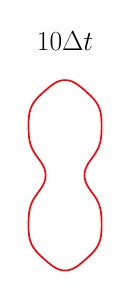
\begin{tikzpicture}[scale=0.4]

\begin{axis}[
  xmin = -1,
  xmax = 1,
  ymin = -2,
  ymax = 2,
  scale only axis,
  axis equal image,
  hide axis,
  title = {\Huge$10 \Delta t$}
  ]

\addplot [mark=none,red,line width=1.5] table{
3.3993e-01 -4.9083e-12
3.4024e-01 1.4106e-02
3.4121e-01 2.8819e-02
3.4296e-01 4.4371e-02
3.4555e-01 6.0467e-02
3.4890e-01 7.6387e-02
3.5275e-01 9.1295e-02
3.5679e-01 1.0469e-01
3.6100e-01 1.1702e-01
3.6594e-01 1.3003e-01
3.7263e-01 1.4582e-01
3.8204e-01 1.6555e-01
3.9495e-01 1.8951e-01
4.1185e-01 2.1737e-01
4.3267e-01 2.4843e-01
4.5669e-01 2.8189e-01
4.8256e-01 3.1708e-01
5.0857e-01 3.5338e-01
5.3303e-01 3.9015e-01
5.5464e-01 4.2661e-01
5.7272e-01 4.6186e-01
5.8719e-01 4.9509e-01
5.9844e-01 5.2579e-01
6.0710e-01 5.5393e-01
6.1381e-01 5.7996e-01
6.1912e-01 6.0457e-01
6.2341e-01 6.2845e-01
6.2691e-01 6.5211e-01
6.2979e-01 6.7593e-01
6.3216e-01 7.0041e-01
6.3412e-01 7.2634e-01
6.3574e-01 7.5473e-01
6.3702e-01 7.8657e-01
6.3793e-01 8.2251e-01
6.3836e-01 8.6273e-01
6.3810e-01 9.0690e-01
6.3670e-01 9.5422e-01
6.3350e-01 1.0035e+00
6.2765e-01 1.0532e+00
6.1854e-01 1.1015e+00
6.0606e-01 1.1469e+00
5.9073e-01 1.1881e+00
5.7350e-01 1.2245e+00
5.5530e-01 1.2563e+00
5.3668e-01 1.2842e+00
5.1774e-01 1.3094e+00
4.9824e-01 1.3329e+00
4.7796e-01 1.3553e+00
4.5692e-01 1.3771e+00
4.3539e-01 1.3982e+00
4.1370e-01 1.4187e+00
3.9205e-01 1.4386e+00
3.7028e-01 1.4581e+00
3.4789e-01 1.4779e+00
3.2417e-01 1.4986e+00
2.9849e-01 1.5205e+00
2.7048e-01 1.5435e+00
2.4005e-01 1.5673e+00
2.0736e-01 1.5906e+00
1.7287e-01 1.6122e+00
1.3732e-01 1.6306e+00
1.0164e-01 1.6449e+00
6.6703e-02 1.6548e+00
3.2921e-02 1.6604e+00
-1.6328e-12 1.6622e+00
-3.2921e-02 1.6604e+00
-6.6703e-02 1.6548e+00
-1.0164e-01 1.6449e+00
-1.3732e-01 1.6306e+00
-1.7287e-01 1.6122e+00
-2.0736e-01 1.5906e+00
-2.4005e-01 1.5673e+00
-2.7048e-01 1.5435e+00
-2.9849e-01 1.5205e+00
-3.2417e-01 1.4986e+00
-3.4789e-01 1.4779e+00
-3.7028e-01 1.4581e+00
-3.9205e-01 1.4386e+00
-4.1370e-01 1.4187e+00
-4.3539e-01 1.3982e+00
-4.5692e-01 1.3771e+00
-4.7796e-01 1.3553e+00
-4.9824e-01 1.3329e+00
-5.1774e-01 1.3094e+00
-5.3668e-01 1.2842e+00
-5.5530e-01 1.2563e+00
-5.7350e-01 1.2245e+00
-5.9073e-01 1.1881e+00
-6.0606e-01 1.1469e+00
-6.1854e-01 1.1015e+00
-6.2765e-01 1.0532e+00
-6.3350e-01 1.0035e+00
-6.3670e-01 9.5422e-01
-6.3810e-01 9.0690e-01
-6.3836e-01 8.6273e-01
-6.3793e-01 8.2251e-01
-6.3702e-01 7.8657e-01
-6.3574e-01 7.5473e-01
-6.3412e-01 7.2634e-01
-6.3216e-01 7.0041e-01
-6.2979e-01 6.7593e-01
-6.2691e-01 6.5211e-01
-6.2341e-01 6.2845e-01
-6.1912e-01 6.0457e-01
-6.1381e-01 5.7996e-01
-6.0710e-01 5.5393e-01
-5.9844e-01 5.2579e-01
-5.8719e-01 4.9509e-01
-5.7272e-01 4.6186e-01
-5.5464e-01 4.2661e-01
-5.3303e-01 3.9015e-01
-5.0857e-01 3.5338e-01
-4.8256e-01 3.1708e-01
-4.5669e-01 2.8189e-01
-4.3267e-01 2.4843e-01
-4.1185e-01 2.1737e-01
-3.9495e-01 1.8951e-01
-3.8204e-01 1.6555e-01
-3.7263e-01 1.4582e-01
-3.6594e-01 1.3003e-01
-3.6100e-01 1.1702e-01
-3.5679e-01 1.0469e-01
-3.5275e-01 9.1295e-02
-3.4890e-01 7.6387e-02
-3.4555e-01 6.0467e-02
-3.4296e-01 4.4371e-02
-3.4121e-01 2.8819e-02
-3.4024e-01 1.4106e-02
-3.3993e-01 -4.2429e-12
-3.4024e-01 -1.4106e-02
-3.4121e-01 -2.8819e-02
-3.4296e-01 -4.4371e-02
-3.4555e-01 -6.0467e-02
-3.4890e-01 -7.6387e-02
-3.5275e-01 -9.1295e-02
-3.5679e-01 -1.0469e-01
-3.6100e-01 -1.1702e-01
-3.6594e-01 -1.3003e-01
-3.7263e-01 -1.4582e-01
-3.8204e-01 -1.6555e-01
-3.9495e-01 -1.8951e-01
-4.1185e-01 -2.1737e-01
-4.3267e-01 -2.4843e-01
-4.5669e-01 -2.8189e-01
-4.8256e-01 -3.1708e-01
-5.0857e-01 -3.5338e-01
-5.3303e-01 -3.9015e-01
-5.5464e-01 -4.2661e-01
-5.7272e-01 -4.6186e-01
-5.8719e-01 -4.9509e-01
-5.9844e-01 -5.2579e-01
-6.0710e-01 -5.5393e-01
-6.1381e-01 -5.7996e-01
-6.1912e-01 -6.0457e-01
-6.2341e-01 -6.2845e-01
-6.2691e-01 -6.5211e-01
-6.2979e-01 -6.7593e-01
-6.3216e-01 -7.0041e-01
-6.3412e-01 -7.2634e-01
-6.3574e-01 -7.5473e-01
-6.3702e-01 -7.8657e-01
-6.3793e-01 -8.2251e-01
-6.3836e-01 -8.6273e-01
-6.3810e-01 -9.0690e-01
-6.3670e-01 -9.5422e-01
-6.3350e-01 -1.0035e+00
-6.2765e-01 -1.0532e+00
-6.1854e-01 -1.1015e+00
-6.0606e-01 -1.1469e+00
-5.9073e-01 -1.1881e+00
-5.7350e-01 -1.2245e+00
-5.5530e-01 -1.2563e+00
-5.3668e-01 -1.2842e+00
-5.1774e-01 -1.3094e+00
-4.9824e-01 -1.3329e+00
-4.7796e-01 -1.3553e+00
-4.5692e-01 -1.3771e+00
-4.3539e-01 -1.3982e+00
-4.1370e-01 -1.4187e+00
-3.9205e-01 -1.4386e+00
-3.7028e-01 -1.4581e+00
-3.4789e-01 -1.4779e+00
-3.2417e-01 -1.4986e+00
-2.9849e-01 -1.5205e+00
-2.7048e-01 -1.5435e+00
-2.4005e-01 -1.5673e+00
-2.0736e-01 -1.5906e+00
-1.7287e-01 -1.6122e+00
-1.3732e-01 -1.6306e+00
-1.0164e-01 -1.6449e+00
-6.6703e-02 -1.6548e+00
-3.2921e-02 -1.6604e+00
-1.6410e-12 -1.6622e+00
3.2921e-02 -1.6604e+00
6.6703e-02 -1.6548e+00
1.0164e-01 -1.6449e+00
1.3732e-01 -1.6306e+00
1.7287e-01 -1.6122e+00
2.0736e-01 -1.5906e+00
2.4005e-01 -1.5673e+00
2.7048e-01 -1.5435e+00
2.9849e-01 -1.5205e+00
3.2417e-01 -1.4986e+00
3.4789e-01 -1.4779e+00
3.7028e-01 -1.4581e+00
3.9205e-01 -1.4386e+00
4.1370e-01 -1.4187e+00
4.3539e-01 -1.3982e+00
4.5692e-01 -1.3771e+00
4.7796e-01 -1.3553e+00
4.9824e-01 -1.3329e+00
5.1774e-01 -1.3094e+00
5.3668e-01 -1.2842e+00
5.5530e-01 -1.2563e+00
5.7350e-01 -1.2245e+00
5.9073e-01 -1.1881e+00
6.0606e-01 -1.1469e+00
6.1854e-01 -1.1015e+00
6.2765e-01 -1.0532e+00
6.3350e-01 -1.0035e+00
6.3670e-01 -9.5422e-01
6.3810e-01 -9.0690e-01
6.3836e-01 -8.6273e-01
6.3793e-01 -8.2251e-01
6.3702e-01 -7.8657e-01
6.3574e-01 -7.5473e-01
6.3412e-01 -7.2634e-01
6.3216e-01 -7.0041e-01
6.2979e-01 -6.7593e-01
6.2691e-01 -6.5211e-01
6.2341e-01 -6.2845e-01
6.1912e-01 -6.0457e-01
6.1381e-01 -5.7996e-01
6.0710e-01 -5.5393e-01
5.9844e-01 -5.2579e-01
5.8719e-01 -4.9509e-01
5.7272e-01 -4.6186e-01
5.5464e-01 -4.2661e-01
5.3303e-01 -3.9015e-01
5.0857e-01 -3.5338e-01
4.8256e-01 -3.1708e-01
4.5669e-01 -2.8189e-01
4.3267e-01 -2.4843e-01
4.1185e-01 -2.1737e-01
3.9495e-01 -1.8951e-01
3.8204e-01 -1.6555e-01
3.7263e-01 -1.4582e-01
3.6594e-01 -1.3003e-01
3.6100e-01 -1.1702e-01
3.5679e-01 -1.0469e-01
3.5275e-01 -9.1295e-02
3.4890e-01 -7.6387e-02
3.4555e-01 -6.0467e-02
3.4296e-01 -4.4371e-02
3.4121e-01 -2.8819e-02
3.4024e-01 -1.4106e-02
3.3993e-01 -4.9083e-12
};


\end{axis}

\end{tikzpicture}



 &
    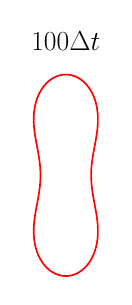
\begin{tikzpicture}[scale=0.4]

\begin{axis}[
  xmin = -1,
  xmax = 1,
  ymin = -2,
  ymax = 2,
  scale only axis,
  axis equal image,
  hide axis,
  title = {\Huge$100 \Delta t$}
  ]

\addplot [mark=none,red,line width=1.5] table{
4.4240e-01 -1.4694e-11
4.4245e-01 1.4110e-02
4.4264e-01 2.8855e-02
4.4297e-01 4.4504e-02
4.4346e-01 6.0802e-02
4.4410e-01 7.7060e-02
4.4485e-01 9.2441e-02
4.4564e-01 1.0642e-01
4.4647e-01 1.1941e-01
4.4746e-01 1.3330e-01
4.4882e-01 1.5040e-01
4.5076e-01 1.7218e-01
4.5352e-01 1.9927e-01
4.5727e-01 2.3165e-01
4.6214e-01 2.6875e-01
4.6812e-01 3.0952e-01
4.7505e-01 3.5266e-01
4.8266e-01 3.9668e-01
4.9054e-01 4.4015e-01
4.9831e-01 4.8182e-01
5.0565e-01 5.2076e-01
5.1231e-01 5.5640e-01
5.1823e-01 5.8856e-01
5.2342e-01 6.1756e-01
5.2800e-01 6.4405e-01
5.3213e-01 6.6889e-01
5.3594e-01 6.9285e-01
5.3951e-01 7.1651e-01
5.4287e-01 7.4028e-01
5.4607e-01 7.6467e-01
5.4917e-01 7.9049e-01
5.5217e-01 8.1877e-01
5.5502e-01 8.5051e-01
5.5755e-01 8.8637e-01
5.5941e-01 9.2655e-01
5.6020e-01 9.7071e-01
5.5947e-01 1.0181e+00
5.5684e-01 1.0674e+00
5.5211e-01 1.1172e+00
5.4531e-01 1.1659e+00
5.3672e-01 1.2122e+00
5.2679e-01 1.2550e+00
5.1600e-01 1.2938e+00
5.0474e-01 1.3287e+00
4.9320e-01 1.3603e+00
4.8127e-01 1.3894e+00
4.6869e-01 1.4172e+00
4.5519e-01 1.4443e+00
4.4064e-01 1.4709e+00
4.2509e-01 1.4967e+00
4.0868e-01 1.5216e+00
3.9149e-01 1.5455e+00
3.7334e-01 1.5684e+00
3.5375e-01 1.5910e+00
3.3197e-01 1.6137e+00
3.0729e-01 1.6367e+00
2.7924e-01 1.6597e+00
2.4778e-01 1.6821e+00
2.1334e-01 1.7027e+00
1.7684e-01 1.7207e+00
1.3951e-01 1.7352e+00
1.0259e-01 1.7459e+00
6.6981e-02 1.7531e+00
3.2955e-02 1.7571e+00
-3.8018e-12 1.7583e+00
-3.2955e-02 1.7571e+00
-6.6981e-02 1.7531e+00
-1.0259e-01 1.7459e+00
-1.3951e-01 1.7352e+00
-1.7684e-01 1.7207e+00
-2.1334e-01 1.7027e+00
-2.4778e-01 1.6821e+00
-2.7924e-01 1.6597e+00
-3.0729e-01 1.6367e+00
-3.3197e-01 1.6137e+00
-3.5375e-01 1.5910e+00
-3.7334e-01 1.5684e+00
-3.9149e-01 1.5455e+00
-4.0868e-01 1.5216e+00
-4.2509e-01 1.4967e+00
-4.4064e-01 1.4709e+00
-4.5519e-01 1.4443e+00
-4.6869e-01 1.4172e+00
-4.8127e-01 1.3894e+00
-4.9320e-01 1.3603e+00
-5.0474e-01 1.3287e+00
-5.1600e-01 1.2938e+00
-5.2679e-01 1.2550e+00
-5.3672e-01 1.2122e+00
-5.4531e-01 1.1659e+00
-5.5211e-01 1.1172e+00
-5.5684e-01 1.0674e+00
-5.5947e-01 1.0181e+00
-5.6020e-01 9.7071e-01
-5.5941e-01 9.2655e-01
-5.5755e-01 8.8637e-01
-5.5502e-01 8.5051e-01
-5.5217e-01 8.1877e-01
-5.4917e-01 7.9049e-01
-5.4607e-01 7.6467e-01
-5.4287e-01 7.4028e-01
-5.3951e-01 7.1651e-01
-5.3594e-01 6.9285e-01
-5.3213e-01 6.6889e-01
-5.2800e-01 6.4405e-01
-5.2342e-01 6.1756e-01
-5.1823e-01 5.8856e-01
-5.1231e-01 5.5640e-01
-5.0565e-01 5.2076e-01
-4.9831e-01 4.8182e-01
-4.9054e-01 4.4015e-01
-4.8266e-01 3.9668e-01
-4.7505e-01 3.5266e-01
-4.6812e-01 3.0952e-01
-4.6214e-01 2.6875e-01
-4.5727e-01 2.3165e-01
-4.5352e-01 1.9927e-01
-4.5076e-01 1.7218e-01
-4.4882e-01 1.5040e-01
-4.4746e-01 1.3330e-01
-4.4647e-01 1.1941e-01
-4.4564e-01 1.0642e-01
-4.4485e-01 9.2441e-02
-4.4410e-01 7.7060e-02
-4.4346e-01 6.0802e-02
-4.4297e-01 4.4504e-02
-4.4264e-01 2.8855e-02
-4.4245e-01 1.4110e-02
-4.4240e-01 -2.7173e-11
-4.4245e-01 -1.4110e-02
-4.4264e-01 -2.8855e-02
-4.4297e-01 -4.4504e-02
-4.4346e-01 -6.0802e-02
-4.4410e-01 -7.7060e-02
-4.4485e-01 -9.2441e-02
-4.4564e-01 -1.0642e-01
-4.4647e-01 -1.1941e-01
-4.4746e-01 -1.3330e-01
-4.4882e-01 -1.5040e-01
-4.5076e-01 -1.7218e-01
-4.5352e-01 -1.9927e-01
-4.5727e-01 -2.3165e-01
-4.6214e-01 -2.6875e-01
-4.6812e-01 -3.0952e-01
-4.7505e-01 -3.5266e-01
-4.8266e-01 -3.9668e-01
-4.9054e-01 -4.4015e-01
-4.9831e-01 -4.8182e-01
-5.0565e-01 -5.2076e-01
-5.1231e-01 -5.5640e-01
-5.1823e-01 -5.8856e-01
-5.2342e-01 -6.1756e-01
-5.2800e-01 -6.4405e-01
-5.3213e-01 -6.6889e-01
-5.3594e-01 -6.9285e-01
-5.3951e-01 -7.1651e-01
-5.4287e-01 -7.4028e-01
-5.4607e-01 -7.6467e-01
-5.4917e-01 -7.9049e-01
-5.5217e-01 -8.1877e-01
-5.5502e-01 -8.5051e-01
-5.5755e-01 -8.8637e-01
-5.5941e-01 -9.2655e-01
-5.6020e-01 -9.7071e-01
-5.5947e-01 -1.0181e+00
-5.5684e-01 -1.0674e+00
-5.5211e-01 -1.1172e+00
-5.4531e-01 -1.1659e+00
-5.3672e-01 -1.2122e+00
-5.2679e-01 -1.2550e+00
-5.1600e-01 -1.2938e+00
-5.0474e-01 -1.3287e+00
-4.9320e-01 -1.3603e+00
-4.8127e-01 -1.3894e+00
-4.6869e-01 -1.4172e+00
-4.5519e-01 -1.4443e+00
-4.4064e-01 -1.4709e+00
-4.2509e-01 -1.4967e+00
-4.0868e-01 -1.5216e+00
-3.9149e-01 -1.5455e+00
-3.7334e-01 -1.5684e+00
-3.5375e-01 -1.5910e+00
-3.3197e-01 -1.6137e+00
-3.0729e-01 -1.6367e+00
-2.7924e-01 -1.6597e+00
-2.4778e-01 -1.6821e+00
-2.1334e-01 -1.7027e+00
-1.7684e-01 -1.7207e+00
-1.3951e-01 -1.7352e+00
-1.0259e-01 -1.7459e+00
-6.6981e-02 -1.7531e+00
-3.2955e-02 -1.7571e+00
6.1544e-12 -1.7583e+00
3.2955e-02 -1.7571e+00
6.6981e-02 -1.7531e+00
1.0259e-01 -1.7459e+00
1.3951e-01 -1.7352e+00
1.7684e-01 -1.7207e+00
2.1334e-01 -1.7027e+00
2.4778e-01 -1.6821e+00
2.7924e-01 -1.6597e+00
3.0729e-01 -1.6367e+00
3.3197e-01 -1.6137e+00
3.5375e-01 -1.5910e+00
3.7334e-01 -1.5684e+00
3.9149e-01 -1.5455e+00
4.0868e-01 -1.5216e+00
4.2509e-01 -1.4967e+00
4.4064e-01 -1.4709e+00
4.5519e-01 -1.4443e+00
4.6869e-01 -1.4172e+00
4.8127e-01 -1.3894e+00
4.9320e-01 -1.3603e+00
5.0474e-01 -1.3287e+00
5.1600e-01 -1.2938e+00
5.2679e-01 -1.2550e+00
5.3672e-01 -1.2122e+00
5.4531e-01 -1.1659e+00
5.5211e-01 -1.1172e+00
5.5684e-01 -1.0674e+00
5.5947e-01 -1.0181e+00
5.6020e-01 -9.7071e-01
5.5941e-01 -9.2655e-01
5.5755e-01 -8.8637e-01
5.5502e-01 -8.5051e-01
5.5217e-01 -8.1877e-01
5.4917e-01 -7.9049e-01
5.4607e-01 -7.6467e-01
5.4287e-01 -7.4028e-01
5.3951e-01 -7.1651e-01
5.3594e-01 -6.9285e-01
5.3213e-01 -6.6889e-01
5.2800e-01 -6.4405e-01
5.2342e-01 -6.1756e-01
5.1823e-01 -5.8856e-01
5.1231e-01 -5.5640e-01
5.0565e-01 -5.2076e-01
4.9831e-01 -4.8182e-01
4.9054e-01 -4.4015e-01
4.8266e-01 -3.9668e-01
4.7505e-01 -3.5266e-01
4.6812e-01 -3.0952e-01
4.6214e-01 -2.6875e-01
4.5727e-01 -2.3165e-01
4.5352e-01 -1.9927e-01
4.5076e-01 -1.7218e-01
4.4882e-01 -1.5040e-01
4.4746e-01 -1.3330e-01
4.4647e-01 -1.1941e-01
4.4564e-01 -1.0642e-01
4.4485e-01 -9.2441e-02
4.4410e-01 -7.7060e-02
4.4346e-01 -6.0802e-02
4.4297e-01 -4.4504e-02
4.4264e-01 -2.8855e-02
4.4245e-01 -1.4110e-02
4.4240e-01 -1.4694e-11
};


\end{axis}

\end{tikzpicture}



 &
    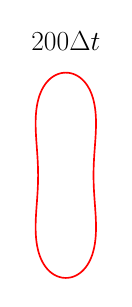
\begin{tikzpicture}[scale=0.4]

\begin{axis}[
  xmin = -1,
  xmax = 1,
  ymin = -2,
  ymax = 2,
  scale only axis,
  axis equal image,
  hide axis,
  title = {\Huge$200 \Delta t$}
  ]

\addplot [mark=none,red,line width=1.5] table{
4.8400e-01 -7.1310e-11
4.8403e-01 1.4110e-02
4.8410e-01 2.8856e-02
4.8423e-01 4.4508e-02
4.8442e-01 6.0812e-02
4.8467e-01 7.7081e-02
4.8496e-01 9.2478e-02
4.8527e-01 1.0647e-01
4.8560e-01 1.1949e-01
4.8599e-01 1.3341e-01
4.8652e-01 1.5056e-01
4.8728e-01 1.7241e-01
4.8837e-01 1.9961e-01
4.8984e-01 2.3218e-01
4.9176e-01 2.6955e-01
4.9412e-01 3.1069e-01
4.9687e-01 3.5429e-01
4.9988e-01 3.9886e-01
5.0300e-01 4.4293e-01
5.0608e-01 4.8522e-01
5.0897e-01 5.2474e-01
5.1158e-01 5.6089e-01
5.1389e-01 5.9352e-01
5.1589e-01 6.2291e-01
5.1764e-01 6.4973e-01
5.1919e-01 6.7487e-01
5.2059e-01 6.9909e-01
5.2188e-01 7.2298e-01
5.2306e-01 7.4696e-01
5.2413e-01 7.7154e-01
5.2511e-01 7.9752e-01
5.2597e-01 8.2595e-01
5.2665e-01 8.5781e-01
5.2703e-01 8.9376e-01
5.2689e-01 9.3398e-01
5.2599e-01 9.7814e-01
5.2406e-01 1.0255e+00
5.2085e-01 1.0747e+00
5.1621e-01 1.1245e+00
5.1016e-01 1.1734e+00
5.0283e-01 1.2199e+00
4.9453e-01 1.2631e+00
4.8556e-01 1.3023e+00
4.7621e-01 1.3378e+00
4.6657e-01 1.3700e+00
4.5655e-01 1.3998e+00
4.4589e-01 1.4284e+00
4.3435e-01 1.4564e+00
4.2179e-01 1.4840e+00
4.0823e-01 1.5109e+00
3.9376e-01 1.5370e+00
3.7843e-01 1.5621e+00
3.6207e-01 1.5863e+00
3.4421e-01 1.6103e+00
3.2413e-01 1.6345e+00
3.0111e-01 1.6592e+00
2.7464e-01 1.6840e+00
2.4458e-01 1.7082e+00
2.1131e-01 1.7307e+00
1.7569e-01 1.7503e+00
1.3895e-01 1.7662e+00
1.0236e-01 1.7781e+00
6.6920e-02 1.7860e+00
3.2947e-02 1.7904e+00
5.5954e-12 1.7918e+00
-3.2947e-02 1.7904e+00
-6.6920e-02 1.7860e+00
-1.0236e-01 1.7781e+00
-1.3895e-01 1.7662e+00
-1.7569e-01 1.7503e+00
-2.1131e-01 1.7307e+00
-2.4458e-01 1.7082e+00
-2.7464e-01 1.6840e+00
-3.0111e-01 1.6592e+00
-3.2413e-01 1.6345e+00
-3.4421e-01 1.6103e+00
-3.6207e-01 1.5863e+00
-3.7843e-01 1.5621e+00
-3.9376e-01 1.5370e+00
-4.0823e-01 1.5109e+00
-4.2179e-01 1.4840e+00
-4.3435e-01 1.4564e+00
-4.4589e-01 1.4284e+00
-4.5655e-01 1.3998e+00
-4.6657e-01 1.3700e+00
-4.7621e-01 1.3378e+00
-4.8556e-01 1.3023e+00
-4.9453e-01 1.2631e+00
-5.0283e-01 1.2199e+00
-5.1016e-01 1.1734e+00
-5.1621e-01 1.1245e+00
-5.2085e-01 1.0747e+00
-5.2406e-01 1.0255e+00
-5.2599e-01 9.7814e-01
-5.2689e-01 9.3398e-01
-5.2703e-01 8.9376e-01
-5.2665e-01 8.5781e-01
-5.2597e-01 8.2595e-01
-5.2511e-01 7.9752e-01
-5.2413e-01 7.7154e-01
-5.2306e-01 7.4696e-01
-5.2188e-01 7.2298e-01
-5.2059e-01 6.9909e-01
-5.1919e-01 6.7487e-01
-5.1764e-01 6.4973e-01
-5.1589e-01 6.2291e-01
-5.1389e-01 5.9352e-01
-5.1158e-01 5.6089e-01
-5.0897e-01 5.2474e-01
-5.0608e-01 4.8522e-01
-5.0300e-01 4.4293e-01
-4.9988e-01 3.9886e-01
-4.9687e-01 3.5429e-01
-4.9412e-01 3.1069e-01
-4.9176e-01 2.6955e-01
-4.8984e-01 2.3218e-01
-4.8837e-01 1.9961e-01
-4.8728e-01 1.7241e-01
-4.8652e-01 1.5056e-01
-4.8599e-01 1.3341e-01
-4.8560e-01 1.1949e-01
-4.8527e-01 1.0647e-01
-4.8496e-01 9.2478e-02
-4.8467e-01 7.7081e-02
-4.8442e-01 6.0812e-02
-4.8423e-01 4.4508e-02
-4.8410e-01 2.8856e-02
-4.8403e-01 1.4110e-02
-4.8400e-01 -8.9612e-11
-4.8403e-01 -1.4110e-02
-4.8410e-01 -2.8856e-02
-4.8423e-01 -4.4508e-02
-4.8442e-01 -6.0812e-02
-4.8467e-01 -7.7081e-02
-4.8496e-01 -9.2478e-02
-4.8527e-01 -1.0647e-01
-4.8560e-01 -1.1949e-01
-4.8599e-01 -1.3341e-01
-4.8652e-01 -1.5056e-01
-4.8728e-01 -1.7241e-01
-4.8837e-01 -1.9961e-01
-4.8984e-01 -2.3218e-01
-4.9176e-01 -2.6955e-01
-4.9412e-01 -3.1069e-01
-4.9687e-01 -3.5429e-01
-4.9988e-01 -3.9886e-01
-5.0300e-01 -4.4293e-01
-5.0608e-01 -4.8522e-01
-5.0897e-01 -5.2474e-01
-5.1158e-01 -5.6089e-01
-5.1389e-01 -5.9352e-01
-5.1589e-01 -6.2291e-01
-5.1764e-01 -6.4973e-01
-5.1919e-01 -6.7487e-01
-5.2059e-01 -6.9909e-01
-5.2188e-01 -7.2298e-01
-5.2306e-01 -7.4696e-01
-5.2413e-01 -7.7154e-01
-5.2511e-01 -7.9752e-01
-5.2597e-01 -8.2595e-01
-5.2665e-01 -8.5781e-01
-5.2703e-01 -8.9376e-01
-5.2689e-01 -9.3398e-01
-5.2599e-01 -9.7814e-01
-5.2406e-01 -1.0255e+00
-5.2085e-01 -1.0747e+00
-5.1621e-01 -1.1245e+00
-5.1016e-01 -1.1734e+00
-5.0283e-01 -1.2199e+00
-4.9453e-01 -1.2631e+00
-4.8556e-01 -1.3023e+00
-4.7621e-01 -1.3378e+00
-4.6657e-01 -1.3700e+00
-4.5655e-01 -1.3998e+00
-4.4589e-01 -1.4284e+00
-4.3435e-01 -1.4564e+00
-4.2179e-01 -1.4840e+00
-4.0823e-01 -1.5109e+00
-3.9376e-01 -1.5370e+00
-3.7843e-01 -1.5621e+00
-3.6207e-01 -1.5863e+00
-3.4421e-01 -1.6103e+00
-3.2413e-01 -1.6345e+00
-3.0111e-01 -1.6592e+00
-2.7464e-01 -1.6840e+00
-2.4458e-01 -1.7082e+00
-2.1131e-01 -1.7307e+00
-1.7569e-01 -1.7503e+00
-1.3895e-01 -1.7662e+00
-1.0236e-01 -1.7781e+00
-6.6920e-02 -1.7860e+00
-3.2947e-02 -1.7904e+00
1.8451e-11 -1.7918e+00
3.2947e-02 -1.7904e+00
6.6920e-02 -1.7860e+00
1.0236e-01 -1.7781e+00
1.3895e-01 -1.7662e+00
1.7569e-01 -1.7503e+00
2.1131e-01 -1.7307e+00
2.4458e-01 -1.7082e+00
2.7464e-01 -1.6840e+00
3.0111e-01 -1.6592e+00
3.2413e-01 -1.6345e+00
3.4421e-01 -1.6103e+00
3.6207e-01 -1.5863e+00
3.7843e-01 -1.5621e+00
3.9376e-01 -1.5370e+00
4.0823e-01 -1.5109e+00
4.2179e-01 -1.4840e+00
4.3435e-01 -1.4564e+00
4.4589e-01 -1.4284e+00
4.5655e-01 -1.3998e+00
4.6657e-01 -1.3700e+00
4.7621e-01 -1.3378e+00
4.8556e-01 -1.3023e+00
4.9453e-01 -1.2631e+00
5.0283e-01 -1.2199e+00
5.1016e-01 -1.1734e+00
5.1621e-01 -1.1245e+00
5.2085e-01 -1.0747e+00
5.2406e-01 -1.0255e+00
5.2599e-01 -9.7814e-01
5.2689e-01 -9.3398e-01
5.2703e-01 -8.9376e-01
5.2665e-01 -8.5781e-01
5.2597e-01 -8.2595e-01
5.2511e-01 -7.9752e-01
5.2413e-01 -7.7154e-01
5.2306e-01 -7.4696e-01
5.2188e-01 -7.2298e-01
5.2059e-01 -6.9909e-01
5.1919e-01 -6.7487e-01
5.1764e-01 -6.4973e-01
5.1589e-01 -6.2291e-01
5.1389e-01 -5.9352e-01
5.1158e-01 -5.6089e-01
5.0897e-01 -5.2474e-01
5.0608e-01 -4.8522e-01
5.0300e-01 -4.4293e-01
4.9988e-01 -3.9886e-01
4.9687e-01 -3.5429e-01
4.9412e-01 -3.1069e-01
4.9176e-01 -2.6955e-01
4.8984e-01 -2.3218e-01
4.8837e-01 -1.9961e-01
4.8728e-01 -1.7241e-01
4.8652e-01 -1.5056e-01
4.8599e-01 -1.3341e-01
4.8560e-01 -1.1949e-01
4.8527e-01 -1.0647e-01
4.8496e-01 -9.2478e-02
4.8467e-01 -7.7081e-02
4.8442e-01 -6.0812e-02
4.8423e-01 -4.4508e-02
4.8410e-01 -2.8856e-02
4.8403e-01 -1.4110e-02
4.8400e-01 -7.1310e-11
};


\end{axis}

\end{tikzpicture}



 &
    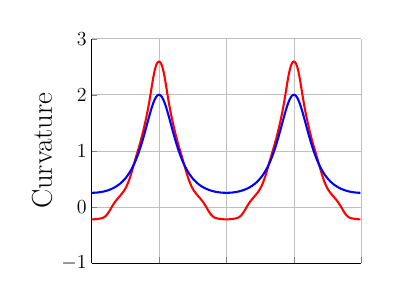
\begin{tikzpicture}[scale=0.5]

\begin{axis}[
  xmin = 0,
  xmax = 6.2832,
  ymin = -1,
  ymax = 3,
  xtick = {0,1.5708,3.1416,4.7124,6.2832},
  xticklabels = {},
  ytick = {-1,0,1,2,3},
  yticklabels = {\Large$-1$,\Large$0$,\Large$1$,\Large$2$,\Large$3$},
  ylabel = {\huge Curvature},
  axis y line* = left,
  axis x line* = bottom,
  grid,
%  legend entries = {$\kappa$,$\tilde{\kappa}$},
%  legend style={at={(0.6,1.1)}, anchor=north west},
%  label style = {draw=none,font=\small},
%  legend cell align = left, 
  ]

\addplot [mark=none,red,line width=1.5] table{
0.0000e+00 -2.2389e-01
2.4544e-02 -2.2329e-01
4.9087e-02 -2.2301e-01
7.3631e-02 -2.2153e-01
9.8175e-02 -2.2008e-01
1.2272e-01 -2.1756e-01
1.4726e-01 -2.1518e-01
1.7181e-01 -2.1216e-01
1.9635e-01 -2.0940e-01
2.2089e-01 -2.0576e-01
2.4544e-01 -2.0101e-01
2.6998e-01 -1.9395e-01
2.9452e-01 -1.8407e-01
3.1907e-01 -1.7035e-01
3.4361e-01 -1.5246e-01
3.6816e-01 -1.3003e-01
3.9270e-01 -1.0358e-01
4.1724e-01 -7.3776e-02
4.4179e-01 -4.2066e-02
4.6633e-01 -9.6424e-03
4.9087e-01 2.1994e-02
5.1542e-01 5.2092e-02
5.3996e-01 7.9833e-02
5.6450e-01 1.0548e-01
5.8905e-01 1.2907e-01
6.1359e-01 1.5165e-01
6.3814e-01 1.7346e-01
6.6268e-01 1.9537e-01
6.8722e-01 2.1742e-01
7.1177e-01 2.4039e-01
7.3631e-01 2.6486e-01
7.6085e-01 2.9205e-01
7.8540e-01 3.2299e-01
8.0994e-01 3.5862e-01
8.3449e-01 3.9956e-01
8.5903e-01 4.4598e-01
8.8357e-01 4.9785e-01
9.0812e-01 5.5462e-01
9.3266e-01 6.1565e-01
9.5720e-01 6.7967e-01
9.8175e-01 7.4555e-01
1.0063e+00 8.1160e-01
1.0308e+00 8.7703e-01
1.0554e+00 9.4068e-01
1.0799e+00 1.0036e+00
1.1045e+00 1.0661e+00
1.1290e+00 1.1312e+00
1.1536e+00 1.1994e+00
1.1781e+00 1.2726e+00
1.2026e+00 1.3493e+00
1.2272e+00 1.4302e+00
1.2517e+00 1.5129e+00
1.2763e+00 1.5999e+00
1.3008e+00 1.6907e+00
1.3254e+00 1.7897e+00
1.3499e+00 1.8960e+00
1.3744e+00 2.0107e+00
1.3990e+00 2.1282e+00
1.4235e+00 2.2442e+00
1.4481e+00 2.3497e+00
1.4726e+00 2.4397e+00
1.4972e+00 2.5083e+00
1.5217e+00 2.5562e+00
1.5463e+00 2.5825e+00
1.5708e+00 2.5919e+00
1.5953e+00 2.5825e+00
1.6199e+00 2.5562e+00
1.6444e+00 2.5083e+00
1.6690e+00 2.4397e+00
1.6935e+00 2.3497e+00
1.7181e+00 2.2442e+00
1.7426e+00 2.1282e+00
1.7671e+00 2.0107e+00
1.7917e+00 1.8960e+00
1.8162e+00 1.7897e+00
1.8408e+00 1.6907e+00
1.8653e+00 1.5999e+00
1.8899e+00 1.5130e+00
1.9144e+00 1.4302e+00
1.9390e+00 1.3493e+00
1.9635e+00 1.2726e+00
1.9880e+00 1.1994e+00
2.0126e+00 1.1312e+00
2.0371e+00 1.0661e+00
2.0617e+00 1.0036e+00
2.0862e+00 9.4068e-01
2.1108e+00 8.7703e-01
2.1353e+00 8.1160e-01
2.1598e+00 7.4555e-01
2.1844e+00 6.7967e-01
2.2089e+00 6.1565e-01
2.2335e+00 5.5462e-01
2.2580e+00 4.9785e-01
2.2826e+00 4.4598e-01
2.3071e+00 3.9956e-01
2.3317e+00 3.5862e-01
2.3562e+00 3.2299e-01
2.3807e+00 2.9205e-01
2.4053e+00 2.6486e-01
2.4298e+00 2.4039e-01
2.4544e+00 2.1742e-01
2.4789e+00 1.9537e-01
2.5035e+00 1.7346e-01
2.5280e+00 1.5165e-01
2.5525e+00 1.2907e-01
2.5771e+00 1.0548e-01
2.6016e+00 7.9833e-02
2.6262e+00 5.2092e-02
2.6507e+00 2.1993e-02
2.6753e+00 -9.6422e-03
2.6998e+00 -4.2066e-02
2.7243e+00 -7.3776e-02
2.7489e+00 -1.0358e-01
2.7734e+00 -1.3003e-01
2.7980e+00 -1.5246e-01
2.8225e+00 -1.7035e-01
2.8471e+00 -1.8407e-01
2.8716e+00 -1.9395e-01
2.8962e+00 -2.0101e-01
2.9207e+00 -2.0576e-01
2.9452e+00 -2.0941e-01
2.9698e+00 -2.1216e-01
2.9943e+00 -2.1518e-01
3.0189e+00 -2.1756e-01
3.0434e+00 -2.2008e-01
3.0680e+00 -2.2153e-01
3.0925e+00 -2.2301e-01
3.1170e+00 -2.2329e-01
3.1416e+00 -2.2389e-01
3.1661e+00 -2.2329e-01
3.1907e+00 -2.2301e-01
3.2152e+00 -2.2153e-01
3.2398e+00 -2.2008e-01
3.2643e+00 -2.1756e-01
3.2889e+00 -2.1518e-01
3.3134e+00 -2.1216e-01
3.3379e+00 -2.0941e-01
3.3625e+00 -2.0576e-01
3.3870e+00 -2.0101e-01
3.4116e+00 -1.9395e-01
3.4361e+00 -1.8407e-01
3.4607e+00 -1.7035e-01
3.4852e+00 -1.5246e-01
3.5097e+00 -1.3003e-01
3.5343e+00 -1.0358e-01
3.5588e+00 -7.3776e-02
3.5834e+00 -4.2067e-02
3.6079e+00 -9.6422e-03
3.6325e+00 2.1993e-02
3.6570e+00 5.2092e-02
3.6816e+00 7.9833e-02
3.7061e+00 1.0548e-01
3.7306e+00 1.2907e-01
3.7552e+00 1.5165e-01
3.7797e+00 1.7346e-01
3.8043e+00 1.9537e-01
3.8288e+00 2.1742e-01
3.8534e+00 2.4039e-01
3.8779e+00 2.6486e-01
3.9024e+00 2.9205e-01
3.9270e+00 3.2299e-01
3.9515e+00 3.5862e-01
3.9761e+00 3.9956e-01
4.0006e+00 4.4598e-01
4.0252e+00 4.9785e-01
4.0497e+00 5.5462e-01
4.0743e+00 6.1565e-01
4.0988e+00 6.7967e-01
4.1233e+00 7.4555e-01
4.1479e+00 8.1160e-01
4.1724e+00 8.7703e-01
4.1970e+00 9.4068e-01
4.2215e+00 1.0036e+00
4.2461e+00 1.0661e+00
4.2706e+00 1.1312e+00
4.2951e+00 1.1994e+00
4.3197e+00 1.2726e+00
4.3442e+00 1.3493e+00
4.3688e+00 1.4302e+00
4.3933e+00 1.5129e+00
4.4179e+00 1.5999e+00
4.4424e+00 1.6907e+00
4.4670e+00 1.7897e+00
4.4915e+00 1.8960e+00
4.5160e+00 2.0107e+00
4.5406e+00 2.1282e+00
4.5651e+00 2.2442e+00
4.5897e+00 2.3497e+00
4.6142e+00 2.4397e+00
4.6388e+00 2.5083e+00
4.6633e+00 2.5562e+00
4.6878e+00 2.5825e+00
4.7124e+00 2.5919e+00
4.7369e+00 2.5825e+00
4.7615e+00 2.5562e+00
4.7860e+00 2.5083e+00
4.8106e+00 2.4397e+00
4.8351e+00 2.3497e+00
4.8597e+00 2.2442e+00
4.8842e+00 2.1282e+00
4.9087e+00 2.0107e+00
4.9333e+00 1.8960e+00
4.9578e+00 1.7897e+00
4.9824e+00 1.6907e+00
5.0069e+00 1.5999e+00
5.0315e+00 1.5129e+00
5.0560e+00 1.4302e+00
5.0805e+00 1.3493e+00
5.1051e+00 1.2726e+00
5.1296e+00 1.1994e+00
5.1542e+00 1.1312e+00
5.1787e+00 1.0661e+00
5.2033e+00 1.0036e+00
5.2278e+00 9.4068e-01
5.2524e+00 8.7703e-01
5.2769e+00 8.1160e-01
5.3014e+00 7.4555e-01
5.3260e+00 6.7967e-01
5.3505e+00 6.1565e-01
5.3751e+00 5.5462e-01
5.3996e+00 4.9785e-01
5.4242e+00 4.4598e-01
5.4487e+00 3.9956e-01
5.4732e+00 3.5862e-01
5.4978e+00 3.2299e-01
5.5223e+00 2.9205e-01
5.5469e+00 2.6486e-01
5.5714e+00 2.4039e-01
5.5960e+00 2.1742e-01
5.6205e+00 1.9537e-01
5.6450e+00 1.7346e-01
5.6696e+00 1.5165e-01
5.6941e+00 1.2907e-01
5.7187e+00 1.0548e-01
5.7432e+00 7.9833e-02
5.7678e+00 5.2092e-02
5.7923e+00 2.1994e-02
5.8169e+00 -9.6423e-03
5.8414e+00 -4.2066e-02
5.8659e+00 -7.3776e-02
5.8905e+00 -1.0358e-01
5.9150e+00 -1.3003e-01
5.9396e+00 -1.5246e-01
5.9641e+00 -1.7035e-01
5.9887e+00 -1.8407e-01
6.0132e+00 -1.9395e-01
6.0377e+00 -2.0101e-01
6.0623e+00 -2.0576e-01
6.0868e+00 -2.0940e-01
6.1114e+00 -2.1216e-01
6.1359e+00 -2.1518e-01
6.1605e+00 -2.1756e-01
6.1850e+00 -2.2008e-01
6.2096e+00 -2.2153e-01
6.2341e+00 -2.2301e-01
6.2586e+00 -2.2329e-01
};

\addplot [mark=none,blue,line width=1.5] table{
0.0000e+00 2.5000e-01
2.4544e-02 2.5017e-01
4.9087e-02 2.5068e-01
7.3631e-02 2.5153e-01
9.8175e-02 2.5273e-01
1.2272e-01 2.5427e-01
1.4726e-01 2.5618e-01
1.7181e-01 2.5845e-01
1.9635e-01 2.6110e-01
2.2089e-01 2.6414e-01
2.4544e-01 2.6757e-01
2.6998e-01 2.7143e-01
2.9452e-01 2.7572e-01
3.1907e-01 2.8047e-01
3.4361e-01 2.8569e-01
3.6816e-01 2.9141e-01
3.9270e-01 2.9767e-01
4.1724e-01 3.0448e-01
4.4179e-01 3.1189e-01
4.6633e-01 3.1993e-01
4.9087e-01 3.2863e-01
5.1542e-01 3.3805e-01
5.3996e-01 3.4823e-01
5.6450e-01 3.5922e-01
5.8905e-01 3.7108e-01
6.1359e-01 3.8388e-01
6.3814e-01 3.9767e-01
6.6268e-01 4.1254e-01
6.8722e-01 4.2856e-01
7.1177e-01 4.4581e-01
7.3631e-01 4.6440e-01
7.6085e-01 4.8442e-01
7.8540e-01 5.0596e-01
8.0994e-01 5.2916e-01
8.3449e-01 5.5412e-01
8.5903e-01 5.8097e-01
8.8357e-01 6.0984e-01
9.0812e-01 6.4087e-01
9.3266e-01 6.7419e-01
9.5720e-01 7.0995e-01
9.8175e-01 7.4826e-01
1.0063e+00 7.8927e-01
1.0308e+00 8.3309e-01
1.0554e+00 8.7982e-01
1.0799e+00 9.2953e-01
1.1045e+00 9.8227e-01
1.1290e+00 1.0380e+00
1.1536e+00 1.0967e+00
1.1781e+00 1.1582e+00
1.2026e+00 1.2223e+00
1.2272e+00 1.2887e+00
1.2517e+00 1.3568e+00
1.2763e+00 1.4263e+00
1.3008e+00 1.4963e+00
1.3254e+00 1.5660e+00
1.3499e+00 1.6345e+00
1.3744e+00 1.7006e+00
1.3990e+00 1.7631e+00
1.4235e+00 1.8208e+00
1.4481e+00 1.8723e+00
1.4726e+00 1.9165e+00
1.4972e+00 1.9523e+00
1.5217e+00 1.9785e+00
1.5463e+00 1.9946e+00
1.5708e+00 2.0000e+00
1.5953e+00 1.9946e+00
1.6199e+00 1.9785e+00
1.6444e+00 1.9523e+00
1.6690e+00 1.9165e+00
1.6935e+00 1.8723e+00
1.7181e+00 1.8208e+00
1.7426e+00 1.7631e+00
1.7671e+00 1.7006e+00
1.7917e+00 1.6345e+00
1.8162e+00 1.5660e+00
1.8408e+00 1.4963e+00
1.8653e+00 1.4263e+00
1.8899e+00 1.3568e+00
1.9144e+00 1.2887e+00
1.9390e+00 1.2223e+00
1.9635e+00 1.1582e+00
1.9880e+00 1.0967e+00
2.0126e+00 1.0380e+00
2.0371e+00 9.8227e-01
2.0617e+00 9.2953e-01
2.0862e+00 8.7982e-01
2.1108e+00 8.3309e-01
2.1353e+00 7.8927e-01
2.1598e+00 7.4826e-01
2.1844e+00 7.0995e-01
2.2089e+00 6.7419e-01
2.2335e+00 6.4087e-01
2.2580e+00 6.0984e-01
2.2826e+00 5.8097e-01
2.3071e+00 5.5412e-01
2.3317e+00 5.2916e-01
2.3562e+00 5.0596e-01
2.3807e+00 4.8442e-01
2.4053e+00 4.6440e-01
2.4298e+00 4.4581e-01
2.4544e+00 4.2856e-01
2.4789e+00 4.1254e-01
2.5035e+00 3.9767e-01
2.5280e+00 3.8388e-01
2.5525e+00 3.7108e-01
2.5771e+00 3.5922e-01
2.6016e+00 3.4823e-01
2.6262e+00 3.3805e-01
2.6507e+00 3.2863e-01
2.6753e+00 3.1993e-01
2.6998e+00 3.1189e-01
2.7243e+00 3.0448e-01
2.7489e+00 2.9767e-01
2.7734e+00 2.9141e-01
2.7980e+00 2.8569e-01
2.8225e+00 2.8047e-01
2.8471e+00 2.7572e-01
2.8716e+00 2.7143e-01
2.8962e+00 2.6757e-01
2.9207e+00 2.6414e-01
2.9452e+00 2.6110e-01
2.9698e+00 2.5845e-01
2.9943e+00 2.5618e-01
3.0189e+00 2.5427e-01
3.0434e+00 2.5273e-01
3.0680e+00 2.5153e-01
3.0925e+00 2.5068e-01
3.1170e+00 2.5017e-01
3.1416e+00 2.5000e-01
3.1661e+00 2.5017e-01
3.1907e+00 2.5068e-01
3.2152e+00 2.5153e-01
3.2398e+00 2.5273e-01
3.2643e+00 2.5427e-01
3.2889e+00 2.5618e-01
3.3134e+00 2.5845e-01
3.3379e+00 2.6110e-01
3.3625e+00 2.6414e-01
3.3870e+00 2.6757e-01
3.4116e+00 2.7143e-01
3.4361e+00 2.7572e-01
3.4607e+00 2.8047e-01
3.4852e+00 2.8569e-01
3.5097e+00 2.9141e-01
3.5343e+00 2.9767e-01
3.5588e+00 3.0448e-01
3.5834e+00 3.1189e-01
3.6079e+00 3.1993e-01
3.6325e+00 3.2863e-01
3.6570e+00 3.3805e-01
3.6816e+00 3.4823e-01
3.7061e+00 3.5922e-01
3.7306e+00 3.7108e-01
3.7552e+00 3.8388e-01
3.7797e+00 3.9767e-01
3.8043e+00 4.1254e-01
3.8288e+00 4.2856e-01
3.8534e+00 4.4581e-01
3.8779e+00 4.6440e-01
3.9024e+00 4.8442e-01
3.9270e+00 5.0596e-01
3.9515e+00 5.2916e-01
3.9761e+00 5.5412e-01
4.0006e+00 5.8097e-01
4.0252e+00 6.0984e-01
4.0497e+00 6.4087e-01
4.0743e+00 6.7419e-01
4.0988e+00 7.0995e-01
4.1233e+00 7.4826e-01
4.1479e+00 7.8927e-01
4.1724e+00 8.3309e-01
4.1970e+00 8.7982e-01
4.2215e+00 9.2953e-01
4.2461e+00 9.8227e-01
4.2706e+00 1.0380e+00
4.2951e+00 1.0967e+00
4.3197e+00 1.1582e+00
4.3442e+00 1.2223e+00
4.3688e+00 1.2887e+00
4.3933e+00 1.3568e+00
4.4179e+00 1.4263e+00
4.4424e+00 1.4963e+00
4.4670e+00 1.5660e+00
4.4915e+00 1.6345e+00
4.5160e+00 1.7006e+00
4.5406e+00 1.7631e+00
4.5651e+00 1.8208e+00
4.5897e+00 1.8723e+00
4.6142e+00 1.9165e+00
4.6388e+00 1.9523e+00
4.6633e+00 1.9785e+00
4.6878e+00 1.9946e+00
4.7124e+00 2.0000e+00
4.7369e+00 1.9946e+00
4.7615e+00 1.9785e+00
4.7860e+00 1.9523e+00
4.8106e+00 1.9165e+00
4.8351e+00 1.8723e+00
4.8597e+00 1.8208e+00
4.8842e+00 1.7631e+00
4.9087e+00 1.7006e+00
4.9333e+00 1.6345e+00
4.9578e+00 1.5660e+00
4.9824e+00 1.4963e+00
5.0069e+00 1.4263e+00
5.0315e+00 1.3568e+00
5.0560e+00 1.2887e+00
5.0805e+00 1.2223e+00
5.1051e+00 1.1582e+00
5.1296e+00 1.0967e+00
5.1542e+00 1.0380e+00
5.1787e+00 9.8227e-01
5.2033e+00 9.2953e-01
5.2278e+00 8.7982e-01
5.2524e+00 8.3309e-01
5.2769e+00 7.8927e-01
5.3014e+00 7.4826e-01
5.3260e+00 7.0995e-01
5.3505e+00 6.7419e-01
5.3751e+00 6.4087e-01
5.3996e+00 6.0984e-01
5.4242e+00 5.8097e-01
5.4487e+00 5.5412e-01
5.4732e+00 5.2916e-01
5.4978e+00 5.0596e-01
5.5223e+00 4.8442e-01
5.5469e+00 4.6440e-01
5.5714e+00 4.4581e-01
5.5960e+00 4.2856e-01
5.6205e+00 4.1254e-01
5.6450e+00 3.9767e-01
5.6696e+00 3.8388e-01
5.6941e+00 3.7108e-01
5.7187e+00 3.5922e-01
5.7432e+00 3.4823e-01
5.7678e+00 3.3805e-01
5.7923e+00 3.2863e-01
5.8169e+00 3.1993e-01
5.8414e+00 3.1189e-01
5.8659e+00 3.0448e-01
5.8905e+00 2.9767e-01
5.9150e+00 2.9141e-01
5.9396e+00 2.8569e-01
5.9641e+00 2.8047e-01
5.9887e+00 2.7572e-01
6.0132e+00 2.7143e-01
6.0377e+00 2.6757e-01
6.0623e+00 2.6414e-01
6.0868e+00 2.6110e-01
6.1114e+00 2.5845e-01
6.1359e+00 2.5618e-01
6.1605e+00 2.5427e-01
6.1850e+00 2.5273e-01
6.2096e+00 2.5153e-01
6.2341e+00 2.5068e-01
6.2586e+00 2.5017e-01
};

\end{axis}

\end{tikzpicture}



 \\

    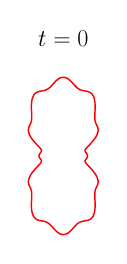
\begin{tikzpicture}[scale=0.35]

\begin{axis}[
  xmin = -1,
  xmax = 1,
  ymin = -2,
  ymax = 2,
  scale only axis,
  axis equal image,
  hide axis,
  title = {\Huge$t=0$}
  ]

\addplot [mark=none,red,line width=1.5] table{
4.8450e-01 0.0000e+00
4.8282e-01 1.3944e-02
4.7797e-01 2.7625e-02
4.7057e-01 4.0837e-02
4.6157e-01 5.3483e-02
4.5216e-01 6.5610e-02
4.4368e-01 7.7429e-02
4.3749e-01 8.9309e-02
4.3482e-01 1.0175e-01
4.3664e-01 1.1536e-01
4.4363e-01 1.3073e-01
4.5602e-01 1.4847e-01
4.7362e-01 1.6902e-01
4.9581e-01 1.9270e-01
5.2161e-01 2.1957e-01
5.4970e-01 2.4946e-01
5.7862e-01 2.8197e-01
6.0680e-01 3.1644e-01
6.3277e-01 3.5209e-01
6.5522e-01 3.8801e-01
6.7317e-01 4.2331e-01
6.8596e-01 4.5717e-01
6.9337e-01 4.8893e-01
6.9559e-01 5.1821e-01
6.9318e-01 5.4490e-01
6.8700e-01 5.6922e-01
6.7816e-01 5.9171e-01
6.6784e-01 6.1317e-01
6.5726e-01 6.3458e-01
6.4746e-01 6.5706e-01
6.3932e-01 6.8170e-01
6.3339e-01 7.0946e-01
6.2991e-01 7.4107e-01
6.2877e-01 7.7696e-01
6.2953e-01 8.1715e-01
6.3150e-01 8.6127e-01
6.3378e-01 9.0854e-01
6.3539e-01 9.5785e-01
6.3533e-01 1.0078e+00
6.3270e-01 1.0569e+00
6.2678e-01 1.1036e+00
6.1707e-01 1.1464e+00
6.0334e-01 1.1842e+00
5.8565e-01 1.2163e+00
5.6432e-01 1.2421e+00
5.3988e-01 1.2618e+00
5.1301e-01 1.2761e+00
4.8448e-01 1.2859e+00
4.5506e-01 1.2925e+00
4.2543e-01 1.2975e+00
3.9616e-01 1.3026e+00
3.6763e-01 1.3092e+00
3.4002e-01 1.3187e+00
3.1334e-01 1.3321e+00
2.8738e-01 1.3498e+00
2.6183e-01 1.3718e+00
2.3629e-01 1.3975e+00
2.1033e-01 1.4261e+00
1.8358e-01 1.4560e+00
1.5574e-01 1.4856e+00
1.2667e-01 1.5130e+00
9.6346e-02 1.5366e+00
6.4922e-02 1.5547e+00
3.2679e-02 1.5661e+00
8.1715e-17 1.5700e+00
-3.2679e-02 1.5661e+00
-6.4922e-02 1.5547e+00
-9.6346e-02 1.5366e+00
-1.2667e-01 1.5130e+00
-1.5574e-01 1.4856e+00
-1.8358e-01 1.4560e+00
-2.1033e-01 1.4261e+00
-2.3629e-01 1.3975e+00
-2.6183e-01 1.3718e+00
-2.8738e-01 1.3498e+00
-3.1334e-01 1.3321e+00
-3.4002e-01 1.3187e+00
-3.6763e-01 1.3092e+00
-3.9616e-01 1.3026e+00
-4.2543e-01 1.2975e+00
-4.5506e-01 1.2925e+00
-4.8448e-01 1.2859e+00
-5.1301e-01 1.2761e+00
-5.3988e-01 1.2618e+00
-5.6432e-01 1.2421e+00
-5.8565e-01 1.2163e+00
-6.0334e-01 1.1842e+00
-6.1707e-01 1.1464e+00
-6.2678e-01 1.1036e+00
-6.3270e-01 1.0569e+00
-6.3533e-01 1.0078e+00
-6.3539e-01 9.5785e-01
-6.3378e-01 9.0854e-01
-6.3150e-01 8.6127e-01
-6.2953e-01 8.1715e-01
-6.2877e-01 7.7696e-01
-6.2991e-01 7.4107e-01
-6.3339e-01 7.0946e-01
-6.3932e-01 6.8170e-01
-6.4746e-01 6.5706e-01
-6.5726e-01 6.3458e-01
-6.6784e-01 6.1317e-01
-6.7816e-01 5.9171e-01
-6.8700e-01 5.6922e-01
-6.9318e-01 5.4490e-01
-6.9559e-01 5.1821e-01
-6.9337e-01 4.8893e-01
-6.8596e-01 4.5717e-01
-6.7317e-01 4.2331e-01
-6.5522e-01 3.8801e-01
-6.3277e-01 3.5209e-01
-6.0680e-01 3.1644e-01
-5.7862e-01 2.8197e-01
-5.4970e-01 2.4946e-01
-5.2161e-01 2.1957e-01
-4.9581e-01 1.9270e-01
-4.7362e-01 1.6902e-01
-4.5602e-01 1.4847e-01
-4.4363e-01 1.3073e-01
-4.3664e-01 1.1536e-01
-4.3482e-01 1.0175e-01
-4.3749e-01 8.9309e-02
-4.4368e-01 7.7429e-02
-4.5216e-01 6.5610e-02
-4.6157e-01 5.3483e-02
-4.7057e-01 4.0837e-02
-4.7797e-01 2.7625e-02
-4.8282e-01 1.3944e-02
-4.8450e-01 6.9805e-17
-4.8282e-01 -1.3944e-02
-4.7797e-01 -2.7625e-02
-4.7057e-01 -4.0837e-02
-4.6157e-01 -5.3483e-02
-4.5216e-01 -6.5610e-02
-4.4368e-01 -7.7429e-02
-4.3749e-01 -8.9309e-02
-4.3482e-01 -1.0175e-01
-4.3664e-01 -1.1536e-01
-4.4363e-01 -1.3073e-01
-4.5602e-01 -1.4847e-01
-4.7362e-01 -1.6902e-01
-4.9581e-01 -1.9270e-01
-5.2161e-01 -2.1957e-01
-5.4970e-01 -2.4946e-01
-5.7862e-01 -2.8197e-01
-6.0680e-01 -3.1644e-01
-6.3277e-01 -3.5209e-01
-6.5522e-01 -3.8801e-01
-6.7317e-01 -4.2331e-01
-6.8596e-01 -4.5717e-01
-6.9337e-01 -4.8893e-01
-6.9559e-01 -5.1821e-01
-6.9318e-01 -5.4490e-01
-6.8700e-01 -5.6922e-01
-6.7816e-01 -5.9171e-01
-6.6784e-01 -6.1317e-01
-6.5726e-01 -6.3458e-01
-6.4746e-01 -6.5706e-01
-6.3932e-01 -6.8170e-01
-6.3339e-01 -7.0946e-01
-6.2991e-01 -7.4107e-01
-6.2877e-01 -7.7696e-01
-6.2953e-01 -8.1715e-01
-6.3150e-01 -8.6127e-01
-6.3378e-01 -9.0854e-01
-6.3539e-01 -9.5785e-01
-6.3533e-01 -1.0078e+00
-6.3270e-01 -1.0569e+00
-6.2678e-01 -1.1036e+00
-6.1707e-01 -1.1464e+00
-6.0334e-01 -1.1842e+00
-5.8565e-01 -1.2163e+00
-5.6432e-01 -1.2421e+00
-5.3988e-01 -1.2618e+00
-5.1301e-01 -1.2761e+00
-4.8448e-01 -1.2859e+00
-4.5506e-01 -1.2925e+00
-4.2543e-01 -1.2975e+00
-3.9616e-01 -1.3026e+00
-3.6763e-01 -1.3092e+00
-3.4002e-01 -1.3187e+00
-3.1334e-01 -1.3321e+00
-2.8738e-01 -1.3498e+00
-2.6183e-01 -1.3718e+00
-2.3629e-01 -1.3975e+00
-2.1033e-01 -1.4261e+00
-1.8358e-01 -1.4560e+00
-1.5574e-01 -1.4856e+00
-1.2667e-01 -1.5130e+00
-9.6346e-02 -1.5366e+00
-6.4922e-02 -1.5547e+00
-3.2679e-02 -1.5661e+00
-2.4514e-16 -1.5700e+00
3.2679e-02 -1.5661e+00
6.4922e-02 -1.5547e+00
9.6346e-02 -1.5366e+00
1.2667e-01 -1.5130e+00
1.5574e-01 -1.4856e+00
1.8358e-01 -1.4560e+00
2.1033e-01 -1.4261e+00
2.3629e-01 -1.3975e+00
2.6183e-01 -1.3718e+00
2.8738e-01 -1.3498e+00
3.1334e-01 -1.3321e+00
3.4002e-01 -1.3187e+00
3.6763e-01 -1.3092e+00
3.9616e-01 -1.3026e+00
4.2543e-01 -1.2975e+00
4.5506e-01 -1.2925e+00
4.8448e-01 -1.2859e+00
5.1301e-01 -1.2761e+00
5.3988e-01 -1.2618e+00
5.6432e-01 -1.2421e+00
5.8565e-01 -1.2163e+00
6.0334e-01 -1.1842e+00
6.1707e-01 -1.1464e+00
6.2678e-01 -1.1036e+00
6.3270e-01 -1.0569e+00
6.3533e-01 -1.0078e+00
6.3539e-01 -9.5785e-01
6.3378e-01 -9.0854e-01
6.3150e-01 -8.6127e-01
6.2953e-01 -8.1715e-01
6.2877e-01 -7.7696e-01
6.2991e-01 -7.4107e-01
6.3339e-01 -7.0946e-01
6.3932e-01 -6.8170e-01
6.4746e-01 -6.5706e-01
6.5726e-01 -6.3458e-01
6.6784e-01 -6.1317e-01
6.7816e-01 -5.9171e-01
6.8700e-01 -5.6922e-01
6.9318e-01 -5.4490e-01
6.9559e-01 -5.1821e-01
6.9337e-01 -4.8893e-01
6.8596e-01 -4.5717e-01
6.7317e-01 -4.2331e-01
6.5522e-01 -3.8801e-01
6.3277e-01 -3.5209e-01
6.0680e-01 -3.1644e-01
5.7862e-01 -2.8197e-01
5.4970e-01 -2.4946e-01
5.2161e-01 -2.1957e-01
4.9581e-01 -1.9270e-01
4.7362e-01 -1.6902e-01
4.5602e-01 -1.4847e-01
4.4363e-01 -1.3073e-01
4.3664e-01 -1.1536e-01
4.3482e-01 -1.0175e-01
4.3749e-01 -8.9309e-02
4.4368e-01 -7.7429e-02
4.5216e-01 -6.5610e-02
4.6157e-01 -5.3483e-02
4.7057e-01 -4.0837e-02
4.7797e-01 -2.7625e-02
4.8282e-01 -1.3944e-02
4.8450e-01 0.0000e+00
};


\end{axis}

\end{tikzpicture}



 &
    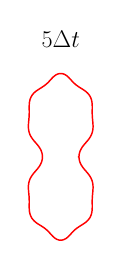
\begin{tikzpicture}[scale=0.35]

\begin{axis}[
  xmin = -1,
  xmax = 1,
  ymin = -2,
  ymax = 2,
  scale only axis,
  axis equal image,
  hide axis,
  title = {\Huge$5\Delta t$}
  ]

\addplot [mark=none,red,line width=1.5] table{
3.6479e-01 -1.7019e-12
3.6513e-01 1.4105e-02
3.6618e-01 2.8813e-02
3.6807e-01 4.4350e-02
3.7089e-01 6.0410e-02
3.7454e-01 7.6266e-02
3.7874e-01 9.1083e-02
3.8316e-01 1.0436e-01
3.8776e-01 1.1654e-01
3.9319e-01 1.2936e-01
4.0055e-01 1.4485e-01
4.1092e-01 1.6409e-01
4.2520e-01 1.8725e-01
4.4395e-01 2.1389e-01
4.6712e-01 2.4324e-01
4.9383e-01 2.7459e-01
5.2247e-01 3.0754e-01
5.5092e-01 3.4195e-01
5.7699e-01 3.7759e-01
5.9896e-01 4.1382e-01
6.1600e-01 4.4957e-01
6.2816e-01 4.8370e-01
6.3619e-01 5.1538e-01
6.4106e-01 5.4441e-01
6.4371e-01 5.7114e-01
6.4480e-01 5.9628e-01
6.4477e-01 6.2053e-01
6.4389e-01 6.4442e-01
6.4236e-01 6.6835e-01
6.4034e-01 6.9285e-01
6.3794e-01 7.1873e-01
6.3527e-01 7.4703e-01
6.3253e-01 7.7876e-01
6.3010e-01 8.1463e-01
6.2846e-01 8.5481e-01
6.2799e-01 8.9898e-01
6.2854e-01 9.4632e-01
6.2908e-01 9.9568e-01
6.2784e-01 1.0457e+00
6.2287e-01 1.0946e+00
6.1290e-01 1.1406e+00
5.9795e-01 1.1819e+00
5.7915e-01 1.2175e+00
5.5802e-01 1.2474e+00
5.3571e-01 1.2725e+00
5.1269e-01 1.2940e+00
4.8891e-01 1.3130e+00
4.6428e-01 1.3305e+00
4.3897e-01 1.3471e+00
4.1339e-01 1.3631e+00
3.8807e-01 1.3788e+00
3.6332e-01 1.3946e+00
3.3910e-01 1.4110e+00
3.1502e-01 1.4287e+00
2.9057e-01 1.4485e+00
2.6548e-01 1.4710e+00
2.3977e-01 1.4966e+00
2.1354e-01 1.5249e+00
1.8669e-01 1.5548e+00
1.5876e-01 1.5843e+00
1.2923e-01 1.6113e+00
9.8014e-02 1.6337e+00
6.5604e-02 1.6499e+00
3.2783e-02 1.6596e+00
1.7115e-12 1.6627e+00
-3.2783e-02 1.6596e+00
-6.5604e-02 1.6499e+00
-9.8014e-02 1.6337e+00
-1.2923e-01 1.6113e+00
-1.5876e-01 1.5843e+00
-1.8669e-01 1.5548e+00
-2.1354e-01 1.5249e+00
-2.3977e-01 1.4966e+00
-2.6548e-01 1.4710e+00
-2.9057e-01 1.4485e+00
-3.1502e-01 1.4287e+00
-3.3910e-01 1.4110e+00
-3.6332e-01 1.3946e+00
-3.8807e-01 1.3788e+00
-4.1339e-01 1.3631e+00
-4.3897e-01 1.3471e+00
-4.6428e-01 1.3305e+00
-4.8891e-01 1.3130e+00
-5.1269e-01 1.2940e+00
-5.3571e-01 1.2725e+00
-5.5802e-01 1.2474e+00
-5.7915e-01 1.2175e+00
-5.9795e-01 1.1819e+00
-6.1290e-01 1.1406e+00
-6.2287e-01 1.0946e+00
-6.2784e-01 1.0457e+00
-6.2908e-01 9.9568e-01
-6.2854e-01 9.4632e-01
-6.2799e-01 8.9898e-01
-6.2846e-01 8.5481e-01
-6.3010e-01 8.1463e-01
-6.3253e-01 7.7876e-01
-6.3527e-01 7.4703e-01
-6.3794e-01 7.1873e-01
-6.4034e-01 6.9285e-01
-6.4236e-01 6.6835e-01
-6.4389e-01 6.4442e-01
-6.4477e-01 6.2053e-01
-6.4480e-01 5.9628e-01
-6.4371e-01 5.7114e-01
-6.4106e-01 5.4441e-01
-6.3619e-01 5.1538e-01
-6.2816e-01 4.8370e-01
-6.1600e-01 4.4957e-01
-5.9896e-01 4.1382e-01
-5.7699e-01 3.7759e-01
-5.5092e-01 3.4195e-01
-5.2247e-01 3.0754e-01
-4.9383e-01 2.7459e-01
-4.6712e-01 2.4324e-01
-4.4395e-01 2.1389e-01
-4.2520e-01 1.8725e-01
-4.1092e-01 1.6409e-01
-4.0055e-01 1.4485e-01
-3.9319e-01 1.2936e-01
-3.8776e-01 1.1654e-01
-3.8316e-01 1.0436e-01
-3.7874e-01 9.1083e-02
-3.7454e-01 7.6266e-02
-3.7089e-01 6.0410e-02
-3.6807e-01 4.4350e-02
-3.6618e-01 2.8813e-02
-3.6513e-01 1.4105e-02
-3.6479e-01 4.4121e-14
-3.6513e-01 -1.4105e-02
-3.6618e-01 -2.8813e-02
-3.6807e-01 -4.4350e-02
-3.7089e-01 -6.0410e-02
-3.7454e-01 -7.6266e-02
-3.7874e-01 -9.1083e-02
-3.8316e-01 -1.0436e-01
-3.8776e-01 -1.1654e-01
-3.9319e-01 -1.2936e-01
-4.0055e-01 -1.4485e-01
-4.1092e-01 -1.6409e-01
-4.2520e-01 -1.8725e-01
-4.4395e-01 -2.1389e-01
-4.6712e-01 -2.4324e-01
-4.9383e-01 -2.7459e-01
-5.2247e-01 -3.0754e-01
-5.5092e-01 -3.4195e-01
-5.7699e-01 -3.7759e-01
-5.9896e-01 -4.1382e-01
-6.1600e-01 -4.4957e-01
-6.2816e-01 -4.8370e-01
-6.3619e-01 -5.1538e-01
-6.4106e-01 -5.4441e-01
-6.4371e-01 -5.7114e-01
-6.4480e-01 -5.9628e-01
-6.4477e-01 -6.2053e-01
-6.4389e-01 -6.4442e-01
-6.4236e-01 -6.6835e-01
-6.4034e-01 -6.9285e-01
-6.3794e-01 -7.1873e-01
-6.3527e-01 -7.4703e-01
-6.3253e-01 -7.7876e-01
-6.3010e-01 -8.1463e-01
-6.2846e-01 -8.5481e-01
-6.2799e-01 -8.9898e-01
-6.2854e-01 -9.4632e-01
-6.2908e-01 -9.9568e-01
-6.2784e-01 -1.0457e+00
-6.2287e-01 -1.0946e+00
-6.1290e-01 -1.1406e+00
-5.9795e-01 -1.1819e+00
-5.7915e-01 -1.2175e+00
-5.5802e-01 -1.2474e+00
-5.3571e-01 -1.2725e+00
-5.1269e-01 -1.2940e+00
-4.8891e-01 -1.3130e+00
-4.6428e-01 -1.3305e+00
-4.3897e-01 -1.3471e+00
-4.1339e-01 -1.3631e+00
-3.8807e-01 -1.3788e+00
-3.6332e-01 -1.3946e+00
-3.3910e-01 -1.4110e+00
-3.1502e-01 -1.4287e+00
-2.9057e-01 -1.4485e+00
-2.6548e-01 -1.4710e+00
-2.3977e-01 -1.4966e+00
-2.1354e-01 -1.5249e+00
-1.8669e-01 -1.5548e+00
-1.5876e-01 -1.5843e+00
-1.2923e-01 -1.6113e+00
-9.8014e-02 -1.6337e+00
-6.5604e-02 -1.6499e+00
-3.2783e-02 -1.6596e+00
-1.5952e-12 -1.6627e+00
3.2783e-02 -1.6596e+00
6.5604e-02 -1.6499e+00
9.8014e-02 -1.6337e+00
1.2923e-01 -1.6113e+00
1.5876e-01 -1.5843e+00
1.8669e-01 -1.5548e+00
2.1354e-01 -1.5249e+00
2.3977e-01 -1.4966e+00
2.6548e-01 -1.4710e+00
2.9057e-01 -1.4485e+00
3.1502e-01 -1.4287e+00
3.3910e-01 -1.4110e+00
3.6332e-01 -1.3946e+00
3.8807e-01 -1.3788e+00
4.1339e-01 -1.3631e+00
4.3897e-01 -1.3471e+00
4.6428e-01 -1.3305e+00
4.8891e-01 -1.3130e+00
5.1269e-01 -1.2940e+00
5.3571e-01 -1.2725e+00
5.5802e-01 -1.2474e+00
5.7915e-01 -1.2175e+00
5.9795e-01 -1.1819e+00
6.1290e-01 -1.1406e+00
6.2287e-01 -1.0946e+00
6.2784e-01 -1.0457e+00
6.2908e-01 -9.9568e-01
6.2854e-01 -9.4632e-01
6.2799e-01 -8.9898e-01
6.2846e-01 -8.5481e-01
6.3010e-01 -8.1463e-01
6.3253e-01 -7.7876e-01
6.3527e-01 -7.4703e-01
6.3794e-01 -7.1873e-01
6.4034e-01 -6.9285e-01
6.4236e-01 -6.6835e-01
6.4389e-01 -6.4442e-01
6.4477e-01 -6.2053e-01
6.4480e-01 -5.9628e-01
6.4371e-01 -5.7114e-01
6.4106e-01 -5.4441e-01
6.3619e-01 -5.1538e-01
6.2816e-01 -4.8370e-01
6.1600e-01 -4.4957e-01
5.9896e-01 -4.1382e-01
5.7699e-01 -3.7759e-01
5.5092e-01 -3.4195e-01
5.2247e-01 -3.0754e-01
4.9383e-01 -2.7459e-01
4.6712e-01 -2.4324e-01
4.4395e-01 -2.1389e-01
4.2520e-01 -1.8725e-01
4.1092e-01 -1.6409e-01
4.0055e-01 -1.4485e-01
3.9319e-01 -1.2936e-01
3.8776e-01 -1.1654e-01
3.8316e-01 -1.0436e-01
3.7874e-01 -9.1083e-02
3.7454e-01 -7.6266e-02
3.7089e-01 -6.0410e-02
3.6807e-01 -4.4350e-02
3.6618e-01 -2.8813e-02
3.6513e-01 -1.4105e-02
3.6479e-01 -1.7019e-12
3.5689e-01 4.3470e-13
3.5723e-01 1.4105e-02
};


\end{axis}

\end{tikzpicture}



 &
    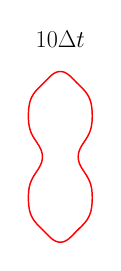
\begin{tikzpicture}[scale=0.35]

\begin{axis}[
  xmin = -1,
  xmax = 1,
  ymin = -2,
  ymax = 2,
  scale only axis,
  axis equal image,
  hide axis,
  title = {\Huge$10 \Delta t$}
  ]

\addplot [mark=none,red,line width=1.5] table{
3.5703e-01 -5.3972e-13
3.5732e-01 1.4107e-02
3.5823e-01 2.8824e-02
3.5988e-01 4.4390e-02
3.6232e-01 6.0512e-02
3.6547e-01 7.6475e-02
3.6910e-01 9.1444e-02
3.7290e-01 1.0491e-01
3.7687e-01 1.1732e-01
3.8152e-01 1.3044e-01
3.8783e-01 1.4639e-01
3.9669e-01 1.6637e-01
4.0885e-01 1.9071e-01
4.2477e-01 2.1915e-01
4.4439e-01 2.5099e-01
4.6701e-01 2.8542e-01
4.9137e-01 3.2167e-01
5.1585e-01 3.5903e-01
5.3887e-01 3.9672e-01
5.5923e-01 4.3389e-01
5.7630e-01 4.6965e-01
5.9001e-01 5.0319e-01
6.0072e-01 5.3409e-01
6.0900e-01 5.6235e-01
6.1544e-01 5.8844e-01
6.2055e-01 6.1309e-01
6.2468e-01 6.3700e-01
6.2805e-01 6.6068e-01
6.3079e-01 6.8452e-01
6.3298e-01 7.0902e-01
6.3471e-01 7.3497e-01
6.3598e-01 7.6337e-01
6.3672e-01 7.9523e-01
6.3680e-01 8.3117e-01
6.3598e-01 8.7139e-01
6.3393e-01 9.1551e-01
6.3016e-01 9.6270e-01
6.2405e-01 1.0117e+00
6.1499e-01 1.0609e+00
6.0264e-01 1.1085e+00
5.8720e-01 1.1530e+00
5.6938e-01 1.1932e+00
5.5020e-01 1.2286e+00
5.3054e-01 1.2596e+00
5.1088e-01 1.2868e+00
4.9121e-01 1.3114e+00
4.7123e-01 1.3344e+00
4.5069e-01 1.3566e+00
4.2961e-01 1.3784e+00
4.0825e-01 1.3997e+00
3.8695e-01 1.4206e+00
3.6592e-01 1.4411e+00
3.4503e-01 1.4616e+00
3.2382e-01 1.4827e+00
3.0168e-01 1.5050e+00
2.7810e-01 1.5292e+00
2.5279e-01 1.5552e+00
2.2565e-01 1.5826e+00
1.9665e-01 1.6104e+00
1.6582e-01 1.6369e+00
1.3338e-01 1.6603e+00
9.9904e-02 1.6791e+00
6.6182e-02 1.6925e+00
3.2856e-02 1.7003e+00
-1.1281e-12 1.7029e+00
-3.2856e-02 1.7003e+00
-6.6182e-02 1.6925e+00
-9.9904e-02 1.6791e+00
-1.3338e-01 1.6603e+00
-1.6582e-01 1.6369e+00
-1.9665e-01 1.6104e+00
-2.2565e-01 1.5826e+00
-2.5279e-01 1.5552e+00
-2.7810e-01 1.5292e+00
-3.0168e-01 1.5050e+00
-3.2382e-01 1.4827e+00
-3.4503e-01 1.4616e+00
-3.6592e-01 1.4411e+00
-3.8695e-01 1.4206e+00
-4.0825e-01 1.3997e+00
-4.2961e-01 1.3784e+00
-4.5069e-01 1.3566e+00
-4.7123e-01 1.3344e+00
-4.9121e-01 1.3114e+00
-5.1088e-01 1.2868e+00
-5.3054e-01 1.2596e+00
-5.5020e-01 1.2286e+00
-5.6938e-01 1.1932e+00
-5.8720e-01 1.1530e+00
-6.0264e-01 1.1085e+00
-6.1499e-01 1.0609e+00
-6.2405e-01 1.0117e+00
-6.3016e-01 9.6270e-01
-6.3393e-01 9.1551e-01
-6.3598e-01 8.7139e-01
-6.3680e-01 8.3117e-01
-6.3672e-01 7.9523e-01
-6.3598e-01 7.6337e-01
-6.3471e-01 7.3497e-01
-6.3298e-01 7.0902e-01
-6.3079e-01 6.8452e-01
-6.2805e-01 6.6068e-01
-6.2468e-01 6.3700e-01
-6.2055e-01 6.1309e-01
-6.1544e-01 5.8844e-01
-6.0900e-01 5.6235e-01
-6.0072e-01 5.3409e-01
-5.9001e-01 5.0319e-01
-5.7630e-01 4.6965e-01
-5.5923e-01 4.3389e-01
-5.3887e-01 3.9672e-01
-5.1585e-01 3.5903e-01
-4.9137e-01 3.2167e-01
-4.6701e-01 2.8542e-01
-4.4439e-01 2.5099e-01
-4.2477e-01 2.1915e-01
-4.0885e-01 1.9071e-01
-3.9669e-01 1.6637e-01
-3.8783e-01 1.4639e-01
-3.8152e-01 1.3044e-01
-3.7687e-01 1.1732e-01
-3.7290e-01 1.0491e-01
-3.6910e-01 9.1444e-02
-3.6547e-01 7.6475e-02
-3.6232e-01 6.0512e-02
-3.5988e-01 4.4390e-02
-3.5823e-01 2.8824e-02
-3.5732e-01 1.4107e-02
-3.5703e-01 -2.2063e-12
-3.5732e-01 -1.4107e-02
-3.5823e-01 -2.8824e-02
-3.5988e-01 -4.4390e-02
-3.6232e-01 -6.0512e-02
-3.6547e-01 -7.6475e-02
-3.6910e-01 -9.1444e-02
-3.7290e-01 -1.0491e-01
-3.7687e-01 -1.1732e-01
-3.8152e-01 -1.3044e-01
-3.8783e-01 -1.4639e-01
-3.9669e-01 -1.6637e-01
-4.0885e-01 -1.9071e-01
-4.2477e-01 -2.1915e-01
-4.4439e-01 -2.5099e-01
-4.6701e-01 -2.8542e-01
-4.9137e-01 -3.2167e-01
-5.1585e-01 -3.5903e-01
-5.3887e-01 -3.9672e-01
-5.5923e-01 -4.3389e-01
-5.7630e-01 -4.6965e-01
-5.9001e-01 -5.0319e-01
-6.0072e-01 -5.3409e-01
-6.0900e-01 -5.6235e-01
-6.1544e-01 -5.8844e-01
-6.2055e-01 -6.1309e-01
-6.2468e-01 -6.3700e-01
-6.2805e-01 -6.6068e-01
-6.3079e-01 -6.8452e-01
-6.3298e-01 -7.0902e-01
-6.3471e-01 -7.3497e-01
-6.3598e-01 -7.6337e-01
-6.3672e-01 -7.9523e-01
-6.3680e-01 -8.3117e-01
-6.3598e-01 -8.7139e-01
-6.3393e-01 -9.1551e-01
-6.3016e-01 -9.6270e-01
-6.2405e-01 -1.0117e+00
-6.1499e-01 -1.0609e+00
-6.0264e-01 -1.1085e+00
-5.8720e-01 -1.1530e+00
-5.6938e-01 -1.1932e+00
-5.5020e-01 -1.2286e+00
-5.3054e-01 -1.2596e+00
-5.1088e-01 -1.2868e+00
-4.9121e-01 -1.3114e+00
-4.7123e-01 -1.3344e+00
-4.5069e-01 -1.3566e+00
-4.2961e-01 -1.3784e+00
-4.0825e-01 -1.3997e+00
-3.8695e-01 -1.4206e+00
-3.6592e-01 -1.4411e+00
-3.4503e-01 -1.4616e+00
-3.2382e-01 -1.4827e+00
-3.0168e-01 -1.5050e+00
-2.7810e-01 -1.5292e+00
-2.5279e-01 -1.5552e+00
-2.2565e-01 -1.5826e+00
-1.9665e-01 -1.6104e+00
-1.6582e-01 -1.6369e+00
-1.3338e-01 -1.6603e+00
-9.9904e-02 -1.6791e+00
-6.6182e-02 -1.6925e+00
-3.2856e-02 -1.7003e+00
-2.8010e-12 -1.7029e+00
3.2856e-02 -1.7003e+00
6.6182e-02 -1.6925e+00
9.9904e-02 -1.6791e+00
1.3338e-01 -1.6603e+00
1.6582e-01 -1.6369e+00
1.9665e-01 -1.6104e+00
2.2565e-01 -1.5826e+00
2.5279e-01 -1.5552e+00
2.7810e-01 -1.5292e+00
3.0168e-01 -1.5050e+00
3.2382e-01 -1.4827e+00
3.4503e-01 -1.4616e+00
3.6592e-01 -1.4411e+00
3.8695e-01 -1.4206e+00
4.0825e-01 -1.3997e+00
4.2961e-01 -1.3784e+00
4.5069e-01 -1.3566e+00
4.7123e-01 -1.3344e+00
4.9121e-01 -1.3114e+00
5.1088e-01 -1.2868e+00
5.3054e-01 -1.2596e+00
5.5020e-01 -1.2286e+00
5.6938e-01 -1.1932e+00
5.8720e-01 -1.1530e+00
6.0264e-01 -1.1085e+00
6.1499e-01 -1.0609e+00
6.2405e-01 -1.0117e+00
6.3016e-01 -9.6270e-01
6.3393e-01 -9.1551e-01
6.3598e-01 -8.7139e-01
6.3680e-01 -8.3117e-01
6.3672e-01 -7.9523e-01
6.3598e-01 -7.6337e-01
6.3471e-01 -7.3497e-01
6.3298e-01 -7.0902e-01
6.3079e-01 -6.8452e-01
6.2805e-01 -6.6068e-01
6.2468e-01 -6.3700e-01
6.2055e-01 -6.1309e-01
6.1544e-01 -5.8844e-01
6.0900e-01 -5.6235e-01
6.0072e-01 -5.3409e-01
5.9001e-01 -5.0319e-01
5.7630e-01 -4.6965e-01
5.5923e-01 -4.3389e-01
5.3887e-01 -3.9672e-01
5.1585e-01 -3.5903e-01
4.9137e-01 -3.2167e-01
4.6701e-01 -2.8542e-01
4.4439e-01 -2.5099e-01
4.2477e-01 -2.1915e-01
4.0885e-01 -1.9071e-01
3.9669e-01 -1.6637e-01
3.8783e-01 -1.4639e-01
3.8152e-01 -1.3044e-01
3.7687e-01 -1.1732e-01
3.7290e-01 -1.0491e-01
3.6910e-01 -9.1444e-02
3.6547e-01 -7.6475e-02
3.6232e-01 -6.0512e-02
3.5988e-01 -4.4390e-02
3.5823e-01 -2.8824e-02
3.5732e-01 -1.4107e-02
3.5703e-01 -5.3972e-13
};


\end{axis}

\end{tikzpicture}



 &
    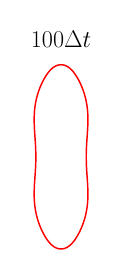
\begin{tikzpicture}[scale=0.35]

\begin{axis}[
  xmin = -1,
  xmax = 1,
  ymin = -2,
  ymax = 2,
  scale only axis,
  axis equal image,
  hide axis,
  title = {\Huge$100 \Delta t$}
  ]

\addplot [mark=none,red,line width=1.5] table{
5.0268e-01 -4.9315e-11
5.0271e-01 1.4110e-02
5.0279e-01 2.8857e-02
5.0295e-01 4.4510e-02
5.0318e-01 6.0817e-02
5.0348e-01 7.7089e-02
5.0382e-01 9.2488e-02
5.0419e-01 1.0648e-01
5.0457e-01 1.1950e-01
5.0503e-01 1.3342e-01
5.0565e-01 1.5056e-01
5.0655e-01 1.7241e-01
5.0780e-01 1.9961e-01
5.0949e-01 2.3218e-01
5.1165e-01 2.6953e-01
5.1425e-01 3.1067e-01
5.1718e-01 3.5426e-01
5.2028e-01 3.9884e-01
5.2335e-01 4.4291e-01
5.2620e-01 4.8521e-01
5.2870e-01 5.2476e-01
5.3078e-01 5.6096e-01
5.3244e-01 5.9362e-01
5.3372e-01 6.2305e-01
5.3468e-01 6.4991e-01
5.3539e-01 6.7508e-01
5.3587e-01 6.9935e-01
5.3614e-01 7.2327e-01
5.3619e-01 7.4727e-01
5.3600e-01 7.7187e-01
5.3551e-01 7.9787e-01
5.3463e-01 8.2630e-01
5.3318e-01 8.5813e-01
5.3093e-01 8.9400e-01
5.2759e-01 9.3409e-01
5.2290e-01 9.7801e-01
5.1662e-01 1.0249e+00
5.0864e-01 1.0737e+00
4.9905e-01 1.1228e+00
4.8810e-01 1.1708e+00
4.7624e-01 1.2163e+00
4.6393e-01 1.2585e+00
4.5160e-01 1.2969e+00
4.3954e-01 1.3315e+00
4.2779e-01 1.3630e+00
4.1616e-01 1.3923e+00
4.0434e-01 1.4204e+00
3.9208e-01 1.4481e+00
3.7926e-01 1.4755e+00
3.6595e-01 1.5026e+00
3.5225e-01 1.5291e+00
3.3820e-01 1.5549e+00
3.2366e-01 1.5804e+00
3.0818e-01 1.6059e+00
2.9117e-01 1.6324e+00
2.7201e-01 1.6602e+00
2.5018e-01 1.6892e+00
2.2539e-01 1.7188e+00
1.9757e-01 1.7477e+00
1.6697e-01 1.7744e+00
1.3424e-01 1.7975e+00
1.0035e-01 1.8155e+00
6.6326e-02 1.8282e+00
3.2874e-02 1.8354e+00
-7.5743e-12 1.8378e+00
-3.2874e-02 1.8354e+00
-6.6326e-02 1.8282e+00
-1.0035e-01 1.8155e+00
-1.3424e-01 1.7975e+00
-1.6697e-01 1.7744e+00
-1.9757e-01 1.7477e+00
-2.2539e-01 1.7188e+00
-2.5018e-01 1.6892e+00
-2.7201e-01 1.6602e+00
-2.9117e-01 1.6324e+00
-3.0818e-01 1.6059e+00
-3.2366e-01 1.5804e+00
-3.3820e-01 1.5549e+00
-3.5225e-01 1.5291e+00
-3.6595e-01 1.5026e+00
-3.7926e-01 1.4755e+00
-3.9208e-01 1.4481e+00
-4.0434e-01 1.4204e+00
-4.1616e-01 1.3923e+00
-4.2779e-01 1.3630e+00
-4.3954e-01 1.3315e+00
-4.5160e-01 1.2969e+00
-4.6393e-01 1.2585e+00
-4.7624e-01 1.2163e+00
-4.8810e-01 1.1708e+00
-4.9905e-01 1.1228e+00
-5.0864e-01 1.0737e+00
-5.1662e-01 1.0249e+00
-5.2290e-01 9.7801e-01
-5.2759e-01 9.3409e-01
-5.3093e-01 8.9400e-01
-5.3318e-01 8.5813e-01
-5.3463e-01 8.2630e-01
-5.3551e-01 7.9787e-01
-5.3600e-01 7.7187e-01
-5.3619e-01 7.4727e-01
-5.3614e-01 7.2327e-01
-5.3587e-01 6.9935e-01
-5.3539e-01 6.7508e-01
-5.3468e-01 6.4991e-01
-5.3372e-01 6.2305e-01
-5.3244e-01 5.9362e-01
-5.3078e-01 5.6096e-01
-5.2870e-01 5.2476e-01
-5.2620e-01 4.8521e-01
-5.2335e-01 4.4291e-01
-5.2028e-01 3.9884e-01
-5.1718e-01 3.5426e-01
-5.1425e-01 3.1067e-01
-5.1165e-01 2.6953e-01
-5.0949e-01 2.3218e-01
-5.0780e-01 1.9961e-01
-5.0655e-01 1.7241e-01
-5.0565e-01 1.5056e-01
-5.0503e-01 1.3342e-01
-5.0457e-01 1.1950e-01
-5.0419e-01 1.0648e-01
-5.0382e-01 9.2488e-02
-5.0348e-01 7.7089e-02
-5.0318e-01 6.0817e-02
-5.0295e-01 4.4510e-02
-5.0279e-01 2.8857e-02
-5.0271e-01 1.4110e-02
-5.0268e-01 -6.3582e-11
-5.0271e-01 -1.4110e-02
-5.0279e-01 -2.8857e-02
-5.0295e-01 -4.4510e-02
-5.0318e-01 -6.0817e-02
-5.0348e-01 -7.7089e-02
-5.0382e-01 -9.2488e-02
-5.0419e-01 -1.0648e-01
-5.0457e-01 -1.1950e-01
-5.0503e-01 -1.3342e-01
-5.0565e-01 -1.5056e-01
-5.0655e-01 -1.7241e-01
-5.0780e-01 -1.9961e-01
-5.0949e-01 -2.3218e-01
-5.1165e-01 -2.6953e-01
-5.1425e-01 -3.1067e-01
-5.1718e-01 -3.5426e-01
-5.2028e-01 -3.9884e-01
-5.2335e-01 -4.4291e-01
-5.2620e-01 -4.8521e-01
-5.2870e-01 -5.2476e-01
-5.3078e-01 -5.6096e-01
-5.3244e-01 -5.9362e-01
-5.3372e-01 -6.2305e-01
-5.3468e-01 -6.4991e-01
-5.3539e-01 -6.7508e-01
-5.3587e-01 -6.9935e-01
-5.3614e-01 -7.2327e-01
-5.3619e-01 -7.4727e-01
-5.3600e-01 -7.7187e-01
-5.3551e-01 -7.9787e-01
-5.3463e-01 -8.2630e-01
-5.3318e-01 -8.5813e-01
-5.3093e-01 -8.9400e-01
-5.2759e-01 -9.3409e-01
-5.2290e-01 -9.7801e-01
-5.1662e-01 -1.0249e+00
-5.0864e-01 -1.0737e+00
-4.9905e-01 -1.1228e+00
-4.8810e-01 -1.1708e+00
-4.7624e-01 -1.2163e+00
-4.6393e-01 -1.2585e+00
-4.5160e-01 -1.2969e+00
-4.3954e-01 -1.3315e+00
-4.2779e-01 -1.3630e+00
-4.1616e-01 -1.3923e+00
-4.0434e-01 -1.4204e+00
-3.9208e-01 -1.4481e+00
-3.7926e-01 -1.4755e+00
-3.6595e-01 -1.5026e+00
-3.5225e-01 -1.5291e+00
-3.3820e-01 -1.5549e+00
-3.2366e-01 -1.5804e+00
-3.0818e-01 -1.6059e+00
-2.9117e-01 -1.6324e+00
-2.7201e-01 -1.6602e+00
-2.5018e-01 -1.6892e+00
-2.2539e-01 -1.7188e+00
-1.9757e-01 -1.7477e+00
-1.6697e-01 -1.7744e+00
-1.3424e-01 -1.7975e+00
-1.0035e-01 -1.8155e+00
-6.6326e-02 -1.8282e+00
-3.2874e-02 -1.8354e+00
7.2992e-12 -1.8378e+00
3.2874e-02 -1.8354e+00
6.6326e-02 -1.8282e+00
1.0035e-01 -1.8155e+00
1.3424e-01 -1.7975e+00
1.6697e-01 -1.7744e+00
1.9757e-01 -1.7477e+00
2.2539e-01 -1.7188e+00
2.5018e-01 -1.6892e+00
2.7201e-01 -1.6602e+00
2.9117e-01 -1.6324e+00
3.0818e-01 -1.6059e+00
3.2366e-01 -1.5804e+00
3.3820e-01 -1.5549e+00
3.5225e-01 -1.5291e+00
3.6595e-01 -1.5026e+00
3.7926e-01 -1.4755e+00
3.9208e-01 -1.4481e+00
4.0434e-01 -1.4204e+00
4.1616e-01 -1.3923e+00
4.2779e-01 -1.3630e+00
4.3954e-01 -1.3315e+00
4.5160e-01 -1.2969e+00
4.6393e-01 -1.2585e+00
4.7624e-01 -1.2163e+00
4.8810e-01 -1.1708e+00
4.9905e-01 -1.1228e+00
5.0864e-01 -1.0737e+00
5.1662e-01 -1.0249e+00
5.2290e-01 -9.7801e-01
5.2759e-01 -9.3409e-01
5.3093e-01 -8.9400e-01
5.3318e-01 -8.5813e-01
5.3463e-01 -8.2630e-01
5.3551e-01 -7.9787e-01
5.3600e-01 -7.7187e-01
5.3619e-01 -7.4727e-01
5.3614e-01 -7.2327e-01
5.3587e-01 -6.9935e-01
5.3539e-01 -6.7508e-01
5.3468e-01 -6.4991e-01
5.3372e-01 -6.2305e-01
5.3244e-01 -5.9362e-01
5.3078e-01 -5.6096e-01
5.2870e-01 -5.2476e-01
5.2620e-01 -4.8521e-01
5.2335e-01 -4.4291e-01
5.2028e-01 -3.9884e-01
5.1718e-01 -3.5426e-01
5.1425e-01 -3.1067e-01
5.1165e-01 -2.6953e-01
5.0949e-01 -2.3218e-01
5.0780e-01 -1.9961e-01
5.0655e-01 -1.7241e-01
5.0565e-01 -1.5056e-01
5.0503e-01 -1.3342e-01
5.0457e-01 -1.1950e-01
5.0419e-01 -1.0648e-01
5.0382e-01 -9.2488e-02
5.0348e-01 -7.7089e-02
5.0318e-01 -6.0817e-02
5.0295e-01 -4.4510e-02
5.0279e-01 -2.8857e-02
5.0271e-01 -1.4110e-02
5.0268e-01 -4.9315e-11
};


\end{axis}

\end{tikzpicture}



 &
    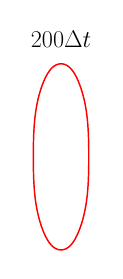
\begin{tikzpicture}[scale=0.35]

\begin{axis}[
  xmin = -1,
  xmax = 1,
  ymin = -2,
  ymax = 2,
  scale only axis,
  axis equal image,
  hide axis,
  title = {\Huge$200 \Delta t$}
  ]

\addplot [mark=none,red,line width=1.5] table{
5.5314e-01 -2.4761e-10
5.5314e-01 1.4110e-02
5.5312e-01 2.8857e-02
5.5308e-01 4.4511e-02
5.5303e-01 6.0820e-02
5.5295e-01 7.7094e-02
5.5287e-01 9.2497e-02
5.5277e-01 1.0650e-01
5.5268e-01 1.1952e-01
5.5256e-01 1.3344e-01
5.5240e-01 1.5060e-01
5.5215e-01 1.7247e-01
5.5180e-01 1.9969e-01
5.5130e-01 2.3230e-01
5.5060e-01 2.6971e-01
5.4968e-01 3.1092e-01
5.4850e-01 3.5460e-01
5.4707e-01 3.9925e-01
5.4539e-01 4.4340e-01
5.4351e-01 4.8576e-01
5.4150e-01 5.2534e-01
5.3942e-01 5.6153e-01
5.3733e-01 5.9418e-01
5.3528e-01 6.2356e-01
5.3324e-01 6.5036e-01
5.3119e-01 6.7546e-01
5.2908e-01 6.9963e-01
5.2687e-01 7.2346e-01
5.2450e-01 7.4734e-01
5.2193e-01 7.7181e-01
5.1905e-01 7.9765e-01
5.1568e-01 8.2589e-01
5.1164e-01 8.5750e-01
5.0674e-01 8.9311e-01
5.0079e-01 9.3289e-01
4.9369e-01 9.7649e-01
4.8538e-01 1.0231e+00
4.7592e-01 1.0716e+00
4.6548e-01 1.1205e+00
4.5433e-01 1.1685e+00
4.4283e-01 1.2141e+00
4.3134e-01 1.2566e+00
4.2013e-01 1.2953e+00
4.0937e-01 1.3303e+00
3.9902e-01 1.3623e+00
3.8886e-01 1.3921e+00
3.7861e-01 1.4208e+00
3.6801e-01 1.4492e+00
3.5695e-01 1.4774e+00
3.4546e-01 1.5053e+00
3.3361e-01 1.5327e+00
3.2142e-01 1.5594e+00
3.0872e-01 1.5858e+00
2.9512e-01 1.6124e+00
2.8003e-01 1.6400e+00
2.6285e-01 1.6691e+00
2.4303e-01 1.6995e+00
2.2016e-01 1.7306e+00
1.9406e-01 1.7611e+00
1.6488e-01 1.7893e+00
1.3317e-01 1.8137e+00
9.9903e-02 1.8330e+00
6.6199e-02 1.8464e+00
3.2859e-02 1.8541e+00
-2.2110e-11 1.8566e+00
-3.2859e-02 1.8541e+00
-6.6199e-02 1.8464e+00
-9.9903e-02 1.8330e+00
-1.3317e-01 1.8137e+00
-1.6488e-01 1.7893e+00
-1.9406e-01 1.7611e+00
-2.2016e-01 1.7306e+00
-2.4303e-01 1.6995e+00
-2.6285e-01 1.6691e+00
-2.8003e-01 1.6400e+00
-2.9512e-01 1.6124e+00
-3.0872e-01 1.5858e+00
-3.2142e-01 1.5594e+00
-3.3361e-01 1.5327e+00
-3.4546e-01 1.5053e+00
-3.5695e-01 1.4774e+00
-3.6801e-01 1.4492e+00
-3.7861e-01 1.4208e+00
-3.8886e-01 1.3921e+00
-3.9902e-01 1.3623e+00
-4.0937e-01 1.3303e+00
-4.2013e-01 1.2953e+00
-4.3134e-01 1.2566e+00
-4.4283e-01 1.2141e+00
-4.5433e-01 1.1685e+00
-4.6548e-01 1.1205e+00
-4.7592e-01 1.0716e+00
-4.8538e-01 1.0231e+00
-4.9369e-01 9.7649e-01
-5.0079e-01 9.3289e-01
-5.0674e-01 8.9311e-01
-5.1164e-01 8.5750e-01
-5.1568e-01 8.2589e-01
-5.1905e-01 7.9765e-01
-5.2193e-01 7.7181e-01
-5.2450e-01 7.4734e-01
-5.2687e-01 7.2346e-01
-5.2908e-01 6.9963e-01
-5.3119e-01 6.7546e-01
-5.3324e-01 6.5036e-01
-5.3528e-01 6.2356e-01
-5.3733e-01 5.9418e-01
-5.3942e-01 5.6153e-01
-5.4150e-01 5.2534e-01
-5.4351e-01 4.8576e-01
-5.4539e-01 4.4340e-01
-5.4707e-01 3.9925e-01
-5.4850e-01 3.5460e-01
-5.4968e-01 3.1092e-01
-5.5060e-01 2.6971e-01
-5.5130e-01 2.3230e-01
-5.5180e-01 1.9969e-01
-5.5215e-01 1.7247e-01
-5.5240e-01 1.5060e-01
-5.5256e-01 1.3344e-01
-5.5268e-01 1.1952e-01
-5.5277e-01 1.0650e-01
-5.5287e-01 9.2497e-02
-5.5295e-01 7.7094e-02
-5.5303e-01 6.0820e-02
-5.5308e-01 4.4511e-02
-5.5312e-01 2.8857e-02
-5.5314e-01 1.4110e-02
-5.5314e-01 -2.7764e-10
-5.5314e-01 -1.4110e-02
-5.5312e-01 -2.8857e-02
-5.5308e-01 -4.4511e-02
-5.5303e-01 -6.0820e-02
-5.5295e-01 -7.7094e-02
-5.5287e-01 -9.2497e-02
-5.5277e-01 -1.0650e-01
-5.5268e-01 -1.1952e-01
-5.5256e-01 -1.3344e-01
-5.5240e-01 -1.5060e-01
-5.5215e-01 -1.7247e-01
-5.5180e-01 -1.9969e-01
-5.5130e-01 -2.3230e-01
-5.5060e-01 -2.6971e-01
-5.4968e-01 -3.1092e-01
-5.4850e-01 -3.5460e-01
-5.4707e-01 -3.9925e-01
-5.4539e-01 -4.4340e-01
-5.4351e-01 -4.8576e-01
-5.4150e-01 -5.2534e-01
-5.3942e-01 -5.6153e-01
-5.3733e-01 -5.9418e-01
-5.3528e-01 -6.2356e-01
-5.3324e-01 -6.5036e-01
-5.3119e-01 -6.7546e-01
-5.2908e-01 -6.9963e-01
-5.2687e-01 -7.2346e-01
-5.2450e-01 -7.4734e-01
-5.2193e-01 -7.7181e-01
-5.1905e-01 -7.9765e-01
-5.1568e-01 -8.2589e-01
-5.1164e-01 -8.5750e-01
-5.0674e-01 -8.9311e-01
-5.0079e-01 -9.3289e-01
-4.9369e-01 -9.7649e-01
-4.8538e-01 -1.0231e+00
-4.7592e-01 -1.0716e+00
-4.6548e-01 -1.1205e+00
-4.5433e-01 -1.1685e+00
-4.4283e-01 -1.2141e+00
-4.3134e-01 -1.2566e+00
-4.2013e-01 -1.2953e+00
-4.0937e-01 -1.3303e+00
-3.9902e-01 -1.3623e+00
-3.8886e-01 -1.3921e+00
-3.7861e-01 -1.4208e+00
-3.6801e-01 -1.4492e+00
-3.5695e-01 -1.4774e+00
-3.4546e-01 -1.5053e+00
-3.3361e-01 -1.5327e+00
-3.2142e-01 -1.5594e+00
-3.0872e-01 -1.5858e+00
-2.9512e-01 -1.6124e+00
-2.8003e-01 -1.6400e+00
-2.6285e-01 -1.6691e+00
-2.4303e-01 -1.6995e+00
-2.2016e-01 -1.7306e+00
-1.9406e-01 -1.7611e+00
-1.6488e-01 -1.7893e+00
-1.3317e-01 -1.8137e+00
-9.9903e-02 -1.8330e+00
-6.6199e-02 -1.8464e+00
-3.2859e-02 -1.8541e+00
2.4249e-11 -1.8566e+00
3.2859e-02 -1.8541e+00
6.6199e-02 -1.8464e+00
9.9903e-02 -1.8330e+00
1.3317e-01 -1.8137e+00
1.6488e-01 -1.7893e+00
1.9406e-01 -1.7611e+00
2.2016e-01 -1.7306e+00
2.4303e-01 -1.6995e+00
2.6285e-01 -1.6691e+00
2.8003e-01 -1.6400e+00
2.9512e-01 -1.6124e+00
3.0872e-01 -1.5858e+00
3.2142e-01 -1.5594e+00
3.3361e-01 -1.5327e+00
3.4546e-01 -1.5053e+00
3.5695e-01 -1.4774e+00
3.6801e-01 -1.4492e+00
3.7861e-01 -1.4208e+00
3.8886e-01 -1.3921e+00
3.9902e-01 -1.3623e+00
4.0937e-01 -1.3303e+00
4.2013e-01 -1.2953e+00
4.3134e-01 -1.2566e+00
4.4283e-01 -1.2141e+00
4.5433e-01 -1.1685e+00
4.6548e-01 -1.1205e+00
4.7592e-01 -1.0716e+00
4.8538e-01 -1.0231e+00
4.9369e-01 -9.7649e-01
5.0079e-01 -9.3289e-01
5.0674e-01 -8.9311e-01
5.1164e-01 -8.5750e-01
5.1568e-01 -8.2589e-01
5.1905e-01 -7.9765e-01
5.2193e-01 -7.7181e-01
5.2450e-01 -7.4734e-01
5.2687e-01 -7.2346e-01
5.2908e-01 -6.9963e-01
5.3119e-01 -6.7546e-01
5.3324e-01 -6.5036e-01
5.3528e-01 -6.2356e-01
5.3733e-01 -5.9418e-01
5.3942e-01 -5.6153e-01
5.4150e-01 -5.2534e-01
5.4351e-01 -4.8576e-01
5.4539e-01 -4.4340e-01
5.4707e-01 -3.9925e-01
5.4850e-01 -3.5460e-01
5.4968e-01 -3.1092e-01
5.5060e-01 -2.6971e-01
5.5130e-01 -2.3230e-01
5.5180e-01 -1.9969e-01
5.5215e-01 -1.7247e-01
5.5240e-01 -1.5060e-01
5.5256e-01 -1.3344e-01
5.5268e-01 -1.1952e-01
5.5277e-01 -1.0650e-01
5.5287e-01 -9.2497e-02
5.5295e-01 -7.7094e-02
5.5303e-01 -6.0820e-02
5.5308e-01 -4.4511e-02
5.5312e-01 -2.8857e-02
5.5314e-01 -1.4110e-02
5.5314e-01 -2.4761e-10
};


\end{axis}

\end{tikzpicture}



 &
    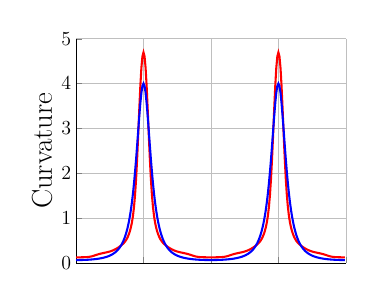
\begin{tikzpicture}[scale=0.5]

\begin{axis}[
  xmin = 0,
  xmax = 6.2832,
  ymin = 0,
  ymax = 5,
  xtick = {0,1.5708,3.1416,4.7124,6.2832},
  xticklabels = {},
  ytick = {0,1,2,3,4,5},
  yticklabels =
  {\Large$0$,\Large$1$,\Large$2$,\Large$3$,\Large$4$,\Large$5$},
  ylabel = {\huge Curvature},
  axis y line* = left,
  axis x line* = bottom,
  grid,
%  legend entries = {$\kappa$,$\tilde{\kappa}$},
%  legend style={at={(0.6,1.1)}, anchor=north west},
%  label style = {draw=none,font=\small},
%  legend cell align = left, 
  ]

\addplot [mark=none,red,line width=1.5] table{
0.0000e+00 1.2309e-01
2.4544e-02 1.2281e-01
4.9087e-02 1.2327e-01
7.3631e-02 1.2330e-01
9.8175e-02 1.2396e-01
1.2272e-01 1.2430e-01
1.4726e-01 1.2517e-01
1.7181e-01 1.2563e-01
1.9635e-01 1.2658e-01
2.2089e-01 1.2728e-01
2.4544e-01 1.2859e-01
2.6998e-01 1.3024e-01
2.9452e-01 1.3276e-01
3.1907e-01 1.3608e-01
3.4361e-01 1.4056e-01
3.6816e-01 1.4604e-01
3.9270e-01 1.5262e-01
4.1724e-01 1.5991e-01
4.4179e-01 1.6777e-01
4.6633e-01 1.7564e-01
4.9087e-01 1.8345e-01
5.1542e-01 1.9065e-01
5.3996e-01 1.9749e-01
5.6450e-01 2.0345e-01
5.8905e-01 2.0928e-01
6.1359e-01 2.1435e-01
6.3814e-01 2.1972e-01
6.6268e-01 2.2451e-01
6.8722e-01 2.2983e-01
7.1177e-01 2.3476e-01
7.3631e-01 2.4045e-01
7.6085e-01 2.4622e-01
7.8540e-01 2.5306e-01
8.0994e-01 2.6048e-01
8.3449e-01 2.6910e-01
8.5903e-01 2.7849e-01
8.8357e-01 2.8905e-01
9.0812e-01 3.0044e-01
9.3266e-01 3.1304e-01
9.5720e-01 3.2656e-01
9.8175e-01 3.4143e-01
1.0063e+00 3.5723e-01
1.0308e+00 3.7447e-01
1.0554e+00 3.9257e-01
1.0799e+00 4.1264e-01
1.1045e+00 4.3443e-01
1.1290e+00 4.6030e-01
1.1536e+00 4.9058e-01
1.1781e+00 5.2836e-01
1.2026e+00 5.7405e-01
1.2272e+00 6.3096e-01
1.2517e+00 7.0004e-01
1.2763e+00 7.8697e-01
1.3008e+00 8.9749e-01
1.3254e+00 1.0452e+00
1.3499e+00 1.2453e+00
1.3744e+00 1.5185e+00
1.3990e+00 1.8799e+00
1.4235e+00 2.3351e+00
1.4481e+00 2.8643e+00
1.4726e+00 3.4217e+00
1.4972e+00 3.9385e+00
1.5217e+00 4.3496e+00
1.5463e+00 4.6073e+00
1.5708e+00 4.6953e+00
1.5953e+00 4.6073e+00
1.6199e+00 4.3496e+00
1.6444e+00 3.9385e+00
1.6690e+00 3.4217e+00
1.6935e+00 2.8643e+00
1.7181e+00 2.3351e+00
1.7426e+00 1.8799e+00
1.7671e+00 1.5185e+00
1.7917e+00 1.2453e+00
1.8162e+00 1.0452e+00
1.8408e+00 8.9749e-01
1.8653e+00 7.8697e-01
1.8899e+00 7.0004e-01
1.9144e+00 6.3096e-01
1.9390e+00 5.7405e-01
1.9635e+00 5.2836e-01
1.9880e+00 4.9058e-01
2.0126e+00 4.6030e-01
2.0371e+00 4.3443e-01
2.0617e+00 4.1264e-01
2.0862e+00 3.9257e-01
2.1108e+00 3.7447e-01
2.1353e+00 3.5723e-01
2.1598e+00 3.4143e-01
2.1844e+00 3.2656e-01
2.2089e+00 3.1304e-01
2.2335e+00 3.0044e-01
2.2580e+00 2.8905e-01
2.2826e+00 2.7849e-01
2.3071e+00 2.6910e-01
2.3317e+00 2.6048e-01
2.3562e+00 2.5306e-01
2.3807e+00 2.4622e-01
2.4053e+00 2.4045e-01
2.4298e+00 2.3475e-01
2.4544e+00 2.2983e-01
2.4789e+00 2.2451e-01
2.5035e+00 2.1972e-01
2.5280e+00 2.1435e-01
2.5525e+00 2.0928e-01
2.5771e+00 2.0345e-01
2.6016e+00 1.9749e-01
2.6262e+00 1.9065e-01
2.6507e+00 1.8345e-01
2.6753e+00 1.7564e-01
2.6998e+00 1.6777e-01
2.7243e+00 1.5991e-01
2.7489e+00 1.5262e-01
2.7734e+00 1.4604e-01
2.7980e+00 1.4056e-01
2.8225e+00 1.3608e-01
2.8471e+00 1.3276e-01
2.8716e+00 1.3024e-01
2.8962e+00 1.2859e-01
2.9207e+00 1.2727e-01
2.9452e+00 1.2658e-01
2.9698e+00 1.2563e-01
2.9943e+00 1.2517e-01
3.0189e+00 1.2430e-01
3.0434e+00 1.2396e-01
3.0680e+00 1.2330e-01
3.0925e+00 1.2327e-01
3.1170e+00 1.2281e-01
3.1416e+00 1.2309e-01
3.1661e+00 1.2281e-01
3.1907e+00 1.2327e-01
3.2152e+00 1.2329e-01
3.2398e+00 1.2396e-01
3.2643e+00 1.2430e-01
3.2889e+00 1.2517e-01
3.3134e+00 1.2563e-01
3.3379e+00 1.2658e-01
3.3625e+00 1.2727e-01
3.3870e+00 1.2859e-01
3.4116e+00 1.3024e-01
3.4361e+00 1.3276e-01
3.4607e+00 1.3608e-01
3.4852e+00 1.4056e-01
3.5097e+00 1.4604e-01
3.5343e+00 1.5262e-01
3.5588e+00 1.5991e-01
3.5834e+00 1.6777e-01
3.6079e+00 1.7564e-01
3.6325e+00 1.8345e-01
3.6570e+00 1.9065e-01
3.6816e+00 1.9749e-01
3.7061e+00 2.0345e-01
3.7306e+00 2.0928e-01
3.7552e+00 2.1435e-01
3.7797e+00 2.1972e-01
3.8043e+00 2.2451e-01
3.8288e+00 2.2983e-01
3.8534e+00 2.3475e-01
3.8779e+00 2.4045e-01
3.9024e+00 2.4622e-01
3.9270e+00 2.5306e-01
3.9515e+00 2.6048e-01
3.9761e+00 2.6910e-01
4.0006e+00 2.7849e-01
4.0252e+00 2.8905e-01
4.0497e+00 3.0044e-01
4.0743e+00 3.1304e-01
4.0988e+00 3.2656e-01
4.1233e+00 3.4143e-01
4.1479e+00 3.5723e-01
4.1724e+00 3.7447e-01
4.1970e+00 3.9257e-01
4.2215e+00 4.1264e-01
4.2461e+00 4.3443e-01
4.2706e+00 4.6030e-01
4.2951e+00 4.9058e-01
4.3197e+00 5.2836e-01
4.3442e+00 5.7405e-01
4.3688e+00 6.3097e-01
4.3933e+00 7.0003e-01
4.4179e+00 7.8698e-01
4.4424e+00 8.9749e-01
4.4670e+00 1.0452e+00
4.4915e+00 1.2453e+00
4.5160e+00 1.5185e+00
4.5406e+00 1.8799e+00
4.5651e+00 2.3351e+00
4.5897e+00 2.8643e+00
4.6142e+00 3.4217e+00
4.6388e+00 3.9385e+00
4.6633e+00 4.3496e+00
4.6878e+00 4.6073e+00
4.7124e+00 4.6953e+00
4.7369e+00 4.6073e+00
4.7615e+00 4.3496e+00
4.7860e+00 3.9385e+00
4.8106e+00 3.4217e+00
4.8351e+00 2.8643e+00
4.8597e+00 2.3351e+00
4.8842e+00 1.8799e+00
4.9087e+00 1.5185e+00
4.9333e+00 1.2453e+00
4.9578e+00 1.0452e+00
4.9824e+00 8.9749e-01
5.0069e+00 7.8698e-01
5.0315e+00 7.0003e-01
5.0560e+00 6.3097e-01
5.0805e+00 5.7405e-01
5.1051e+00 5.2836e-01
5.1296e+00 4.9058e-01
5.1542e+00 4.6030e-01
5.1787e+00 4.3443e-01
5.2033e+00 4.1264e-01
5.2278e+00 3.9257e-01
5.2524e+00 3.7447e-01
5.2769e+00 3.5723e-01
5.3014e+00 3.4143e-01
5.3260e+00 3.2656e-01
5.3505e+00 3.1304e-01
5.3751e+00 3.0044e-01
5.3996e+00 2.8905e-01
5.4242e+00 2.7849e-01
5.4487e+00 2.6910e-01
5.4732e+00 2.6048e-01
5.4978e+00 2.5306e-01
5.5223e+00 2.4622e-01
5.5469e+00 2.4045e-01
5.5714e+00 2.3475e-01
5.5960e+00 2.2983e-01
5.6205e+00 2.2451e-01
5.6450e+00 2.1972e-01
5.6696e+00 2.1435e-01
5.6941e+00 2.0928e-01
5.7187e+00 2.0345e-01
5.7432e+00 1.9749e-01
5.7678e+00 1.9065e-01
5.7923e+00 1.8345e-01
5.8169e+00 1.7564e-01
5.8414e+00 1.6777e-01
5.8659e+00 1.5991e-01
5.8905e+00 1.5262e-01
5.9150e+00 1.4604e-01
5.9396e+00 1.4056e-01
5.9641e+00 1.3608e-01
5.9887e+00 1.3276e-01
6.0132e+00 1.3024e-01
6.0377e+00 1.2859e-01
6.0623e+00 1.2727e-01
6.0868e+00 1.2658e-01
6.1114e+00 1.2563e-01
6.1359e+00 1.2517e-01
6.1605e+00 1.2430e-01
6.1850e+00 1.2396e-01
6.2096e+00 1.2330e-01
6.2341e+00 1.2327e-01
6.2586e+00 1.2281e-01
};

\addplot [mark=none,blue,line width=1.5] table{
0.0000e+00 6.2500e-02
2.4544e-02 6.2553e-02
4.9087e-02 6.2712e-02
7.3631e-02 6.2979e-02
9.8175e-02 6.3354e-02
1.2272e-01 6.3840e-02
1.4726e-01 6.4441e-02
1.7181e-01 6.5160e-02
1.9635e-01 6.6001e-02
2.2089e-01 6.6970e-02
2.4544e-01 6.8073e-02
2.6998e-01 6.9317e-02
2.9452e-01 7.0711e-02
3.1907e-01 7.2265e-02
3.4361e-01 7.3989e-02
3.6816e-01 7.5895e-02
3.9270e-01 7.7998e-02
4.1724e-01 8.0314e-02
4.4179e-01 8.2860e-02
4.6633e-01 8.5657e-02
4.9087e-01 8.8728e-02
5.1542e-01 9.2099e-02
5.3996e-01 9.5800e-02
5.6450e-01 9.9864e-02
5.8905e-01 1.0433e-01
6.1359e-01 1.0924e-01
6.3814e-01 1.1465e-01
6.6268e-01 1.2061e-01
6.8722e-01 1.2719e-01
7.1177e-01 1.3447e-01
7.3631e-01 1.4253e-01
7.6085e-01 1.5147e-01
7.8540e-01 1.6141e-01
8.0994e-01 1.7249e-01
8.3449e-01 1.8487e-01
8.5903e-01 1.9873e-01
8.8357e-01 2.1429e-01
9.0812e-01 2.3181e-01
9.3266e-01 2.5159e-01
9.5720e-01 2.7399e-01
9.8175e-01 2.9944e-01
1.0063e+00 3.2845e-01
1.0308e+00 3.6161e-01
1.0554e+00 3.9966e-01
1.0799e+00 4.4345e-01
1.1045e+00 4.9401e-01
1.1290e+00 5.5258e-01
1.1536e+00 6.2062e-01
1.1781e+00 6.9985e-01
1.2026e+00 7.9233e-01
1.2272e+00 9.0039e-01
1.2517e+00 1.0267e+00
1.2763e+00 1.1742e+00
1.3008e+00 1.3460e+00
1.3254e+00 1.5449e+00
1.3499e+00 1.7731e+00
1.3744e+00 2.0316e+00
1.3990e+00 2.3186e+00
1.4235e+00 2.6287e+00
1.4481e+00 2.9511e+00
1.4726e+00 3.2686e+00
1.4972e+00 3.5581e+00
1.5217e+00 3.7927e+00
1.5463e+00 3.9464e+00
1.5708e+00 4.0000e+00
1.5953e+00 3.9464e+00
1.6199e+00 3.7927e+00
1.6444e+00 3.5581e+00
1.6690e+00 3.2686e+00
1.6935e+00 2.9511e+00
1.7181e+00 2.6287e+00
1.7426e+00 2.3186e+00
1.7671e+00 2.0316e+00
1.7917e+00 1.7731e+00
1.8162e+00 1.5449e+00
1.8408e+00 1.3460e+00
1.8653e+00 1.1742e+00
1.8899e+00 1.0267e+00
1.9144e+00 9.0039e-01
1.9390e+00 7.9233e-01
1.9635e+00 6.9985e-01
1.9880e+00 6.2062e-01
2.0126e+00 5.5258e-01
2.0371e+00 4.9401e-01
2.0617e+00 4.4345e-01
2.0862e+00 3.9966e-01
2.1108e+00 3.6161e-01
2.1353e+00 3.2845e-01
2.1598e+00 2.9944e-01
2.1844e+00 2.7399e-01
2.2089e+00 2.5159e-01
2.2335e+00 2.3181e-01
2.2580e+00 2.1429e-01
2.2826e+00 1.9873e-01
2.3071e+00 1.8487e-01
2.3317e+00 1.7249e-01
2.3562e+00 1.6141e-01
2.3807e+00 1.5147e-01
2.4053e+00 1.4253e-01
2.4298e+00 1.3447e-01
2.4544e+00 1.2719e-01
2.4789e+00 1.2061e-01
2.5035e+00 1.1465e-01
2.5280e+00 1.0924e-01
2.5525e+00 1.0433e-01
2.5771e+00 9.9864e-02
2.6016e+00 9.5800e-02
2.6262e+00 9.2099e-02
2.6507e+00 8.8728e-02
2.6753e+00 8.5657e-02
2.6998e+00 8.2860e-02
2.7243e+00 8.0314e-02
2.7489e+00 7.7998e-02
2.7734e+00 7.5895e-02
2.7980e+00 7.3989e-02
2.8225e+00 7.2265e-02
2.8471e+00 7.0711e-02
2.8716e+00 6.9317e-02
2.8962e+00 6.8073e-02
2.9207e+00 6.6970e-02
2.9452e+00 6.6001e-02
2.9698e+00 6.5160e-02
2.9943e+00 6.4441e-02
3.0189e+00 6.3840e-02
3.0434e+00 6.3354e-02
3.0680e+00 6.2979e-02
3.0925e+00 6.2712e-02
3.1170e+00 6.2553e-02
3.1416e+00 6.2500e-02
3.1661e+00 6.2553e-02
3.1907e+00 6.2712e-02
3.2152e+00 6.2979e-02
3.2398e+00 6.3354e-02
3.2643e+00 6.3840e-02
3.2889e+00 6.4441e-02
3.3134e+00 6.5160e-02
3.3379e+00 6.6001e-02
3.3625e+00 6.6970e-02
3.3870e+00 6.8073e-02
3.4116e+00 6.9317e-02
3.4361e+00 7.0711e-02
3.4607e+00 7.2265e-02
3.4852e+00 7.3989e-02
3.5097e+00 7.5895e-02
3.5343e+00 7.7998e-02
3.5588e+00 8.0314e-02
3.5834e+00 8.2860e-02
3.6079e+00 8.5657e-02
3.6325e+00 8.8728e-02
3.6570e+00 9.2099e-02
3.6816e+00 9.5800e-02
3.7061e+00 9.9864e-02
3.7306e+00 1.0433e-01
3.7552e+00 1.0924e-01
3.7797e+00 1.1465e-01
3.8043e+00 1.2061e-01
3.8288e+00 1.2719e-01
3.8534e+00 1.3447e-01
3.8779e+00 1.4253e-01
3.9024e+00 1.5147e-01
3.9270e+00 1.6141e-01
3.9515e+00 1.7249e-01
3.9761e+00 1.8487e-01
4.0006e+00 1.9873e-01
4.0252e+00 2.1429e-01
4.0497e+00 2.3181e-01
4.0743e+00 2.5159e-01
4.0988e+00 2.7399e-01
4.1233e+00 2.9944e-01
4.1479e+00 3.2845e-01
4.1724e+00 3.6161e-01
4.1970e+00 3.9966e-01
4.2215e+00 4.4345e-01
4.2461e+00 4.9401e-01
4.2706e+00 5.5258e-01
4.2951e+00 6.2062e-01
4.3197e+00 6.9985e-01
4.3442e+00 7.9233e-01
4.3688e+00 9.0039e-01
4.3933e+00 1.0267e+00
4.4179e+00 1.1742e+00
4.4424e+00 1.3460e+00
4.4670e+00 1.5449e+00
4.4915e+00 1.7731e+00
4.5160e+00 2.0316e+00
4.5406e+00 2.3186e+00
4.5651e+00 2.6287e+00
4.5897e+00 2.9511e+00
4.6142e+00 3.2686e+00
4.6388e+00 3.5581e+00
4.6633e+00 3.7927e+00
4.6878e+00 3.9464e+00
4.7124e+00 4.0000e+00
4.7369e+00 3.9464e+00
4.7615e+00 3.7927e+00
4.7860e+00 3.5581e+00
4.8106e+00 3.2686e+00
4.8351e+00 2.9511e+00
4.8597e+00 2.6287e+00
4.8842e+00 2.3186e+00
4.9087e+00 2.0316e+00
4.9333e+00 1.7731e+00
4.9578e+00 1.5449e+00
4.9824e+00 1.3460e+00
5.0069e+00 1.1742e+00
5.0315e+00 1.0267e+00
5.0560e+00 9.0039e-01
5.0805e+00 7.9233e-01
5.1051e+00 6.9985e-01
5.1296e+00 6.2062e-01
5.1542e+00 5.5258e-01
5.1787e+00 4.9401e-01
5.2033e+00 4.4345e-01
5.2278e+00 3.9966e-01
5.2524e+00 3.6161e-01
5.2769e+00 3.2845e-01
5.3014e+00 2.9944e-01
5.3260e+00 2.7399e-01
5.3505e+00 2.5159e-01
5.3751e+00 2.3181e-01
5.3996e+00 2.1429e-01
5.4242e+00 1.9873e-01
5.4487e+00 1.8487e-01
5.4732e+00 1.7249e-01
5.4978e+00 1.6141e-01
5.5223e+00 1.5147e-01
5.5469e+00 1.4253e-01
5.5714e+00 1.3447e-01
5.5960e+00 1.2719e-01
5.6205e+00 1.2061e-01
5.6450e+00 1.1465e-01
5.6696e+00 1.0924e-01
5.6941e+00 1.0433e-01
5.7187e+00 9.9864e-02
5.7432e+00 9.5800e-02
5.7678e+00 9.2099e-02
5.7923e+00 8.8728e-02
5.8169e+00 8.5657e-02
5.8414e+00 8.2860e-02
5.8659e+00 8.0314e-02
5.8905e+00 7.7998e-02
5.9150e+00 7.5895e-02
5.9396e+00 7.3989e-02
5.9641e+00 7.2265e-02
5.9887e+00 7.0711e-02
6.0132e+00 6.9317e-02
6.0377e+00 6.8073e-02
6.0623e+00 6.6970e-02
6.0868e+00 6.6001e-02
6.1114e+00 6.5160e-02
6.1359e+00 6.4441e-02
6.1605e+00 6.3840e-02
6.1850e+00 6.3354e-02
6.2096e+00 6.2979e-02
6.2341e+00 6.2712e-02
6.2586e+00 6.2553e-02
};

\end{axis}

\end{tikzpicture}




    \fi
  \end{tabular}
\end{center}
\mcaption{Here we show the relaxation dynamics of a single vesicle with
three different prescribed intrinsic curvatures $\tilde{\kappa}$. There
is no imposed background flow.  The vesicle is discretized with $N=256$
points and $\Delta t = 0.02$.  After 200 time steps, the vesicle is
within $0.01 \%$ of its steady state configuration.  The final
curvature (red) and curvature of the intrinsic shape (blue) are in the
right plots.}{f:newbending} 
\end{figure}

